% book example for classicthesis.sty
\documentclass[
  % Replace twoside with oneside if you are printing your thesis on a single side
  % of the paper, or for viewing on screen.
  %oneside,
  oneside,
  11pt, a4paper,
  footinclude=true,
  headinclude=true,
  cleardoublepage=empty
]{scrbook}

\usepackage{xcolor}
\definecolor{nicepurple}{HTML}{B10DC9}
\definecolor{niceblue}{HTML}{0074D9}
\usepackage[colorlinks=true,linkcolor=niceblue,citecolor=nicepurple]{hyperref}

\tolerance=100
\usepackage{lipsum}
\usepackage{graphicx}
\usepackage[linedheaders,parts,pdfspacing]{classicthesis}
\usepackage{acronym}
\usepackage{microtype}
\usepackage[british]{babel}

\usepackage{float}
\usepackage{caption}
\usepackage{subcaption}
\usepackage{gensymb}


\usepackage{amsmath,amsfonts,amsthm,amssymb}
\usepackage[cal=cm]{mathalfa}

\newtheorem{mydef}{Definition}
\newtheorem{myprop}{Property}
\newtheorem{mythm}{Theorem}
\newtheorem{mylem}{Lemma}
\newtheorem{mycor}{Corollary}

\graphicspath{{./Figures/}}


\title{Penrose Aperiodic Tiling of the Plane and Graphical Geodesics}
\author{Jesse Bettencourt\\1144386\\[80pt]  \textit{Supervisor: Dr. Miroslav Lovric}\\[30pt]ISCI 4A12}

\begin{document}

\maketitle

%*******************************************************
% Abstract
%*******************************************************
\pdfbookmark[1]{Abstract}{Abstract}
\chapter*{Abstract}

Short summary of the contents of your thesis.

%*******************************************************
% Dedication
%*******************************************************
\thispagestyle{empty}
\pdfbookmark[1]{Dedication}{Dedication}

\vspace*{3cm}

\begin{center}
    To someone special 
\end{center}

%*******************************************************
% Acknowledgments
%*******************************************************
\pdfbookmark[1]{Acknowledgements}{acknowledgements}
\chapter*{Acknowledgements}

Put your acknowledgements here.

%*******************************************************
% Declaration
%*******************************************************
\pdfbookmark[0]{Declaration}{declaration}
\chapter*{Declaration}
\thispagestyle{empty}

Put your declaration here.


%*******************************************************
% Table of Contents
%*******************************************************
\pdfbookmark[1]{\contentsname}{tableofcontents}

\setcounter{tocdepth}{2} % <-- 2 includes up to subsections in the ToC
\setcounter{secnumdepth}{3} % <-- 3 numbers up to subsubsections

\tableofcontents 

%*******************************************************
% List of Figures and of the Tables
%*******************************************************

%*******************************************************
% List of Figures
%*******************************************************    
\pdfbookmark[1]{\listfigurename}{lof}
\listoffigures





\chapter{Introduction to Tessellations}
\section{Definitions} %DONE 
We will begin our discussion of Penrose tilings with some definitions given by Senechal \cite{Senechal1996}. First, a formal definition of a tiling of Euclidean n-space, $\mathbb{E}^n$:



\begin{mydef}
A \textbf{tiling} $\mathcal{T}$ of the space $\mathbb{E}^n$ is a countable family of closed sets, $T$, called tiles:
\begin{equation*}
\mathcal{T}=\{T_1,T_2,\mathellipsis\}
\end{equation*}
such that
\begin{enumerate}
\item $\mathcal{T}$ has no overlaps: $\mathring{T_i} \cap \mathring{T_j}=\emptyset$ if $i\neq j$
\item $\mathcal{T}$ has no gaps: $\bigcup_{i=1}^\infty T_i = \mathbb{E}^n$
\end{enumerate}
\end{mydef}


Here $\mathring{T}$ denotes the interior of tile $T$. Further, we assume that a tile is the closure of its interior, and that tiles have positive volume. These assumptions allow, for example, a line segment to be a tile in $\mathbb{E}^1$ but not in $\mathbb{E}^2$. Notice that this definition of tiling neither restricts the shape of the individual tiles nor the number of unique tiling shapes.  

However, we will impose some restrictions on the tiles here. Since we are considering tilings of the plane, our tiling must satisfy the above definition for $n=2$, that is, for the Euclidean plane $\mathbb{E}^2$. Further, while the general definition does not impose any criteria on tile shape, for our purposes we will only consider n-dimensional polytopes. In the case of the plane, we consider only 2-polytopes, or polygons. To denote the facets of our tiles we will use \textbf{edges} to denote the 1-dimensional faces, and \textbf{vertices} to denote the 0-dimensional faces. 

\begin{mydef}
Let $\{T_1,T_2,\mathellipsis\}$ be the set of tiles of tiling $\mathcal{T}$, partitioned into a set of equivalence classes by criterion $\mathcal{M}$. The set, $\mathcal{P}$, of representatives of these equivalence classes is called the \textbf{protoset} for $\mathcal{T}$ with respect to $\mathcal{M}$.
\end{mydef}

For example, consider an infinite black-and-white checkerboard (Fig.\ref{fig:checkerboard}). Each tile in the checkerboard is either a black or white square, and the tiling is given by the matching rule that black squares may only share edges with white squares, and vice-versa. In this example, the equivalence class criterion, $\mathcal{M}$, is the colour of the square together with this matching rule. The protoset, $\mathcal{P}$, for the checkerboard is the set containing two elements: a black square and a white square.

\begin{figure}[H]

  \hspace*{\fill}
\begin{subfigure}[t]{0.4\textwidth}
	\includegraphics[width=\textwidth]{Checkerboard}
    \caption{Checkerboard}
    \label{fig:checkerboard}
\end{subfigure}
  \hspace*{\fill}
\begin{subfigure}[t]{0.4\textwidth}
	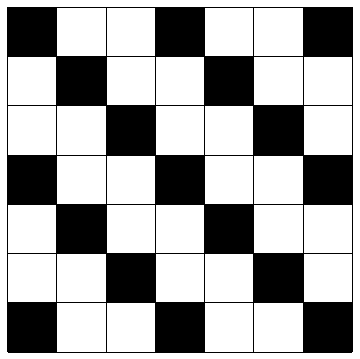
\includegraphics[width=\textwidth]{CheckerboardOther}
    \caption{Different Criterion.}
    \label{fig:critchecker}
\end{subfigure}
  \hspace*{\fill}\\
  \hspace*{\fill}
  \begin{subfigure}[t]{0.4\textwidth}
  	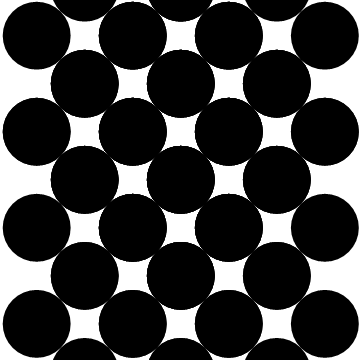
\includegraphics[width=\textwidth]{CheckerboardCircles}
      \caption{Deformed Checkerboard}
      \label{fig:deformedchecker}
  \end{subfigure}
      \hspace*{\fill} 
\begin{subfigure}[t]{0.4\textwidth}
	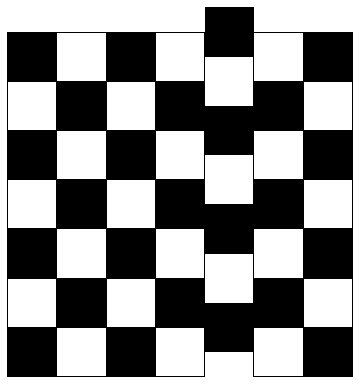
\includegraphics[width=\textwidth]{CheckerboardAperiodic}
    \caption{Sub-Periodic Checkerboard}
    \label{fig:aperiodicchecker}
\end{subfigure} 
\hspace*{\fill}
\label{fig:checker}
\caption[Checkerboard Tilings]{A protoset of black and white squares can admit multiple tilings. Some of them may be periodic, but this is not necessary.}
\end{figure}

\begin{mydef}
If $\mathcal{T}$ is a tiling with protoset $\mathcal{P}$, then we say that $\mathcal{P}$ admits $\mathcal{T}$.
\end{mydef}

In the checkerboard example we say that the protoset containing black and white squares, together with the matching criterion, admits a checkerboard tiling (Fig.\ref{fig:checkerboard}). It is important to note that a protoset can admit multiple tilings given different criterion. For example, the checkerboard protoset also admits the tiling in Fig.\ref{fig:critchecker} under a different matching rule. 

Further, it is also worth noting that abstract criterion, such as colour-matching or directed edges, can be accomplished instead through deformation of the edges of protoset tiles such that the criterion is forced. Consider again the criterion for producing the checkerboard tiling (Fig.\ref{fig:checkerboard}), that black squares may only share edges with white squares, and vice-versa. One way to realize this criterion is to deform all black squares into circles, and to deform white squares into asteroids. As seen in Fig.\ref{fig:deformedchecker}, these deformations force a tiling such that all white tiles occupy the interstices of the black circles. In other words, the protoset of deformed tiles, the black circle and white asteroid, can only admit one unique tiling. We are able to force a checkerboard pattern without any abstract criterion such as colour-matching adjacent tiles. While it is important to understand that abstract matching criterion can be realized by edge deformations, considering simpler protosets with more complicated criterion will usually allow greater insight into the structure and patterns within a tiling than would considering a simple criterion with complicated prototiles. 

\begin{mydef}
A tiling of  $\mathbb{E}^n$ is said to be \textbf{periodic} if it admits translational symmetry in $n$ linearly independent directions.
\end{mydef}

For example, the checkerboard tiling in Fig.\ref{fig:checkerboard} is periodic, as it has translational symmetry in two directions: vertical translation by two units, and horizontal translation by two units. Likewise, we can see that the criterion generating Fig.\ref{fig:critchecker} produces a tiling which is also periodic, with vertical and horizontal translational symmetry given by translation by three units. 

A corollary of a tiling being periodic is that it can be generated by translating a finite subregion by linear combinations of the independent directions. For example, the checkerboard can be generated by infinitely repeating a $2\times2$ subregion translated vertically and horizontally. 

\begin{mydef}
A tiling of  $\mathbb{E}^n$ is said to be \textbf{sub-periodic} if it admits translational symmetry in $k$ linearly independent directions, where $1\leq k\leq n$. A tiling is said to be \textbf{non-periodic} if it admits no translational symmetry. 
\end{mydef}

For example, consider the checkerboard pattern with a single `column' translated vertically by a half-unit distance (Fig.\ref{fig:aperiodicchecker}). This tiling admits translational symmetry in the vertical direction with translation by two units. However, we can see that there is no horizontal symmetry because horizontal translation will not allow the shifted column to overlap anywhere. For this reason, there are also no diagonal translational symmetries admitted. This column shifted checkerboard is sub-periodic. 

Unlike periodic tilings, neither sub-periodic nor non-periodic tilings can be generated by translations of a finite subregion. 

We've seen that the protoset of black and white squares admits multiple types of tiling, both periodic and sub-periodic. Some protosets, such as the circle and asteroid (Fig.\ref{fig:deformedchecker}), only admit tilings which are periodic. A question which motivated the discovery of the Penrose tiles was whether we can find protosets that admit \textit{only} non-periodic tilings.

\begin{mydef}
A protoset $\mathcal{P}$ is said to be \textbf{aperiodic} if it admits only non-periodic tilings. A tiling $\mathcal{T}$ from an aperiodic protoset is called an \textbf{aperiodic tiling}. 
\end{mydef}

Here, `only' means that no subset of the protoset, nor the entire protoset, can tile periodically. 


\section{Kepler's Monsters} 
In 1619, Kepler discovered the third law of planetary motion which he described in his book \textit{Harmonices Mundi} (The Harmonies of the World) \cite{Kepler1997}. While patterns of plane tilings have been known to the ancients, featured widely in art and architecture, it was in Harmonices Mundi where Kepler first provided a mathematical framework with which to discuss these tiling patterns. Primarily, he shows that only 3 polygons are able to regularly tile the plane in singular protosets (Fig. \ref{fig:regular}). That is, using protosets containing only one element, only protosets of equilateral triangles, squares, and hexagons admit plane tilings. 

\begin{figure}[H]
        \centering
        \begin{subfigure}[b]{0.3\textwidth}
                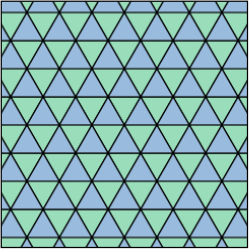
\includegraphics[width=\textwidth]{triangle}
                \caption{Tiling by triangles}
                \label{fig:triangle}
        \end{subfigure}\hfill%
        ~ %add desired spacing between images, e. g. ~, \quad, \qquad, \hfill etc.
          %(or a blank line to force the subfigure onto a new line)
        \begin{subfigure}[b]{0.35\textwidth}
                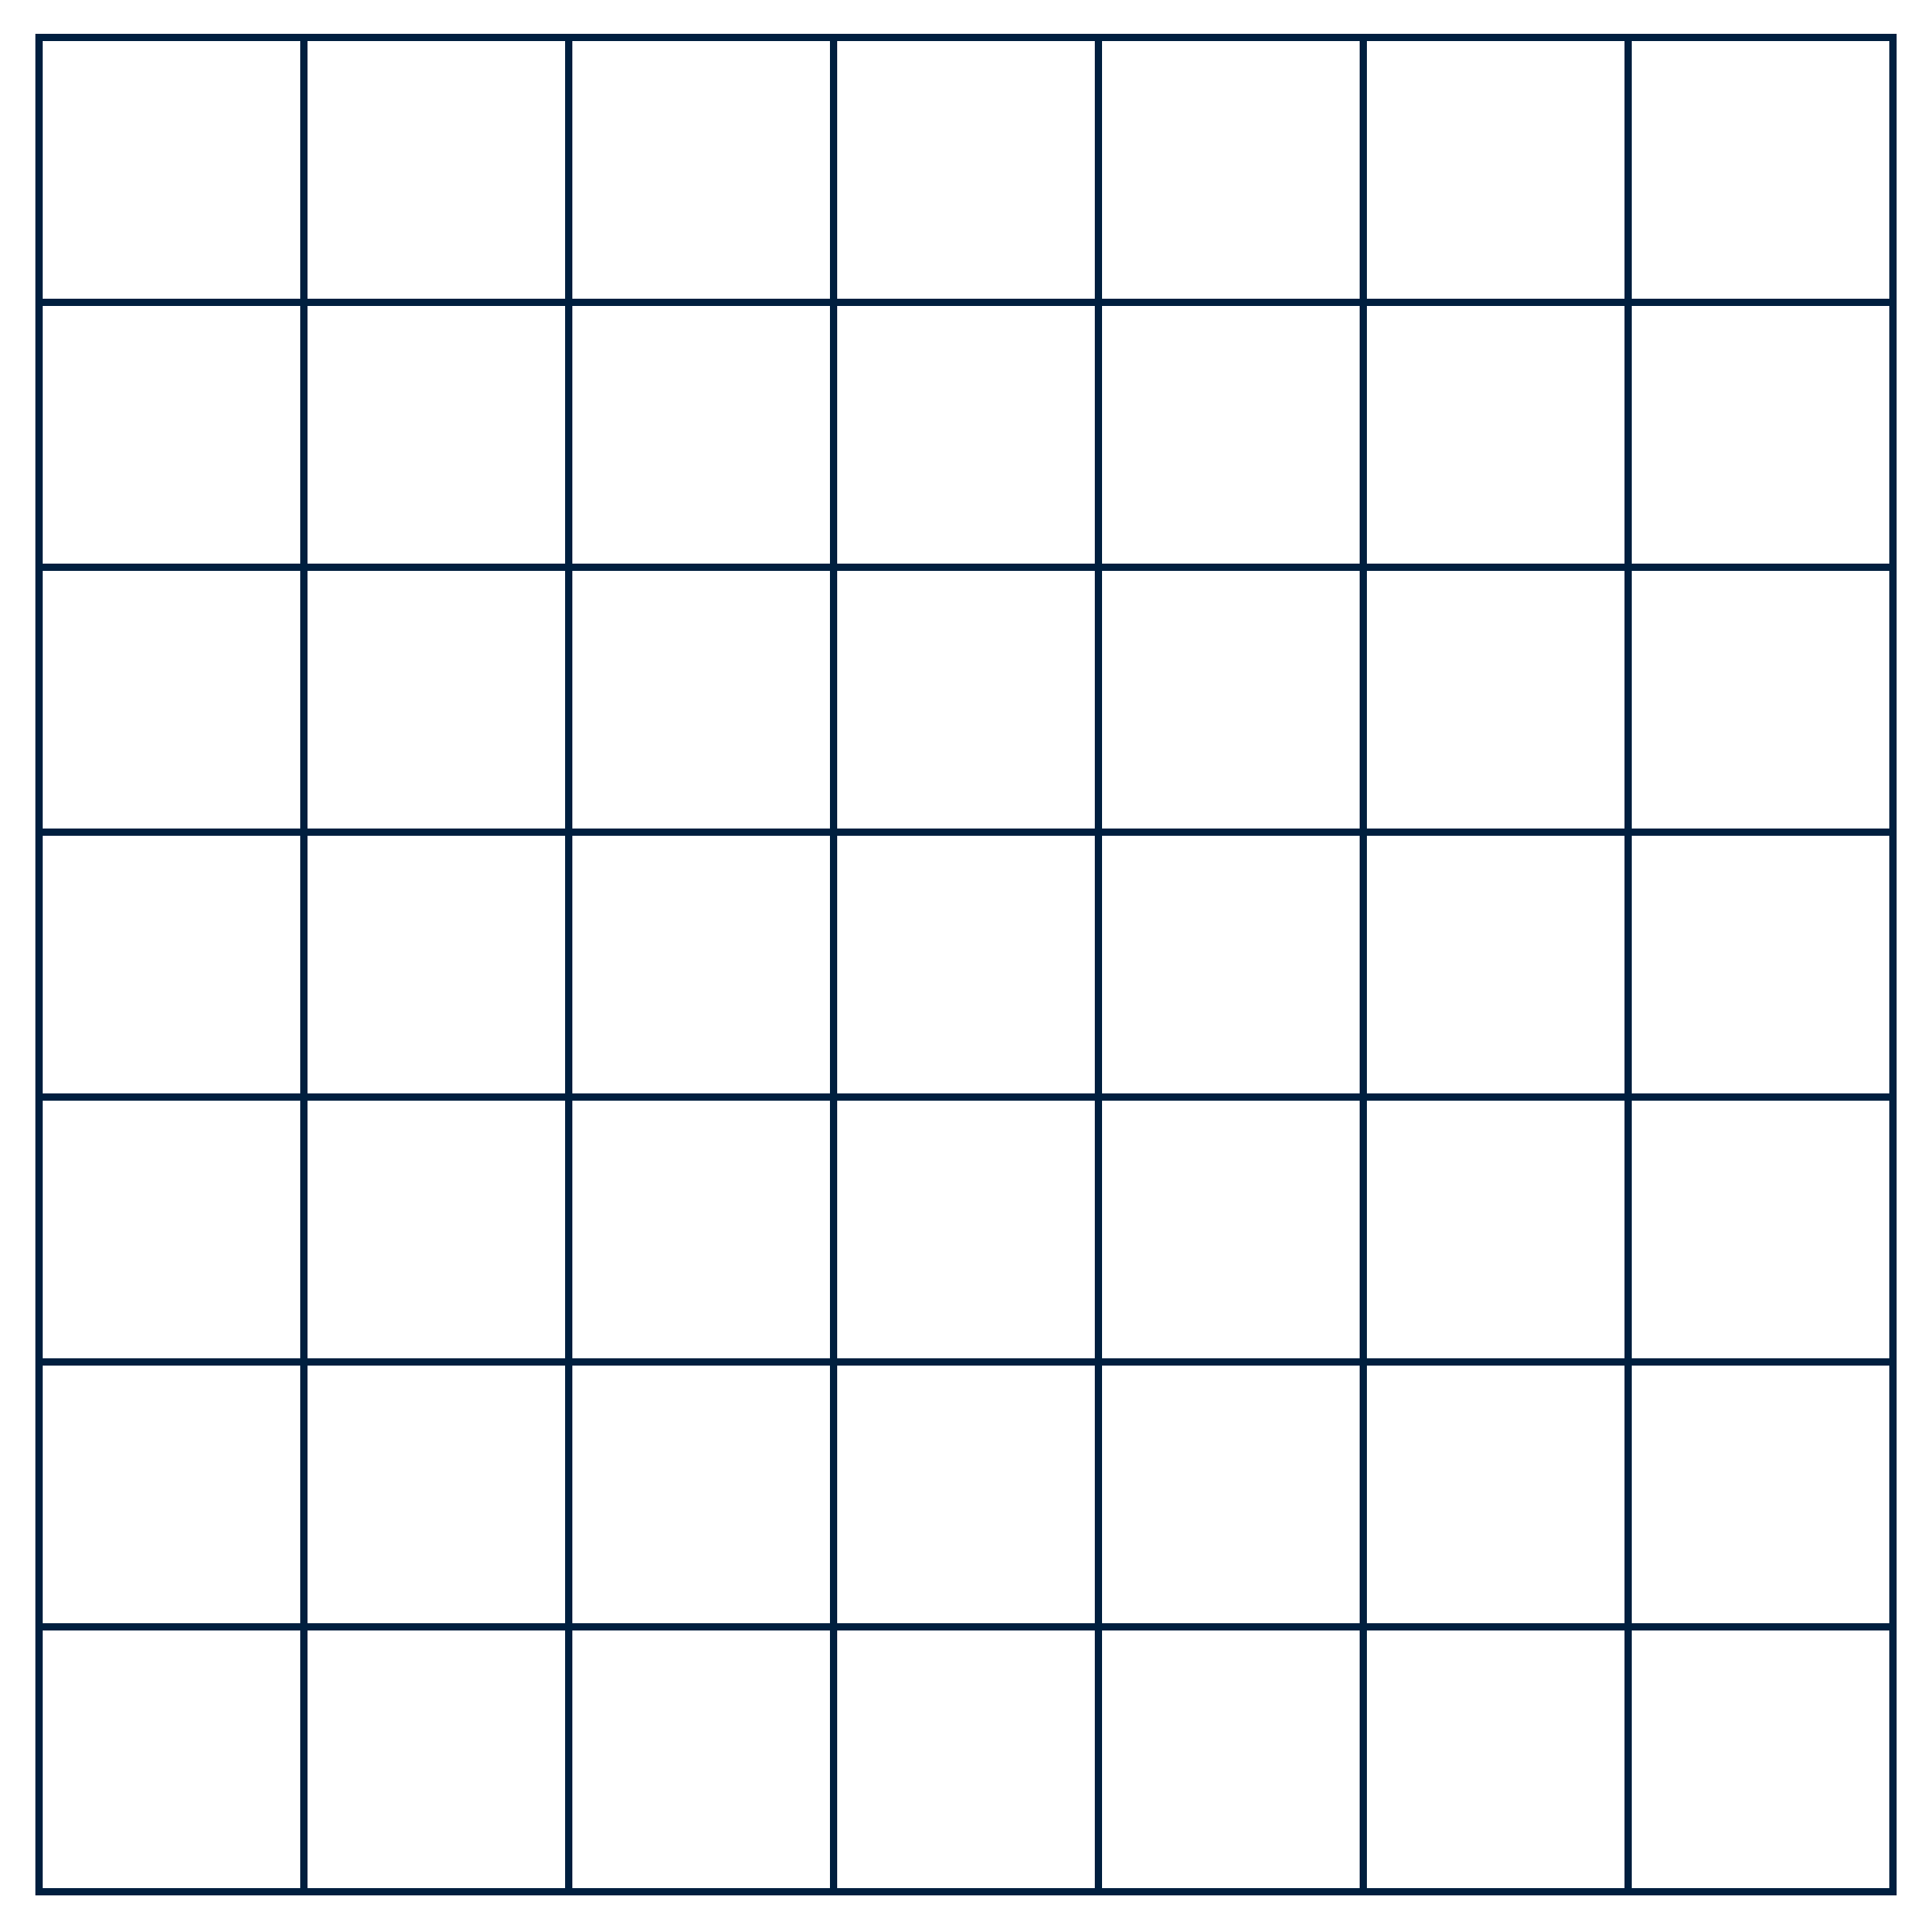
\includegraphics[width=\textwidth]{square}
                \caption{Tiling by squares}
                \label{fig:square}
        \end{subfigure}\hfill
        ~ %add desired spacing between images, e. g. ~, \quad, \qquad, \hfill etc.
          %(or a blank line to force the subfigure onto a new line)
        \begin{subfigure}[b]{0.3\textwidth}
                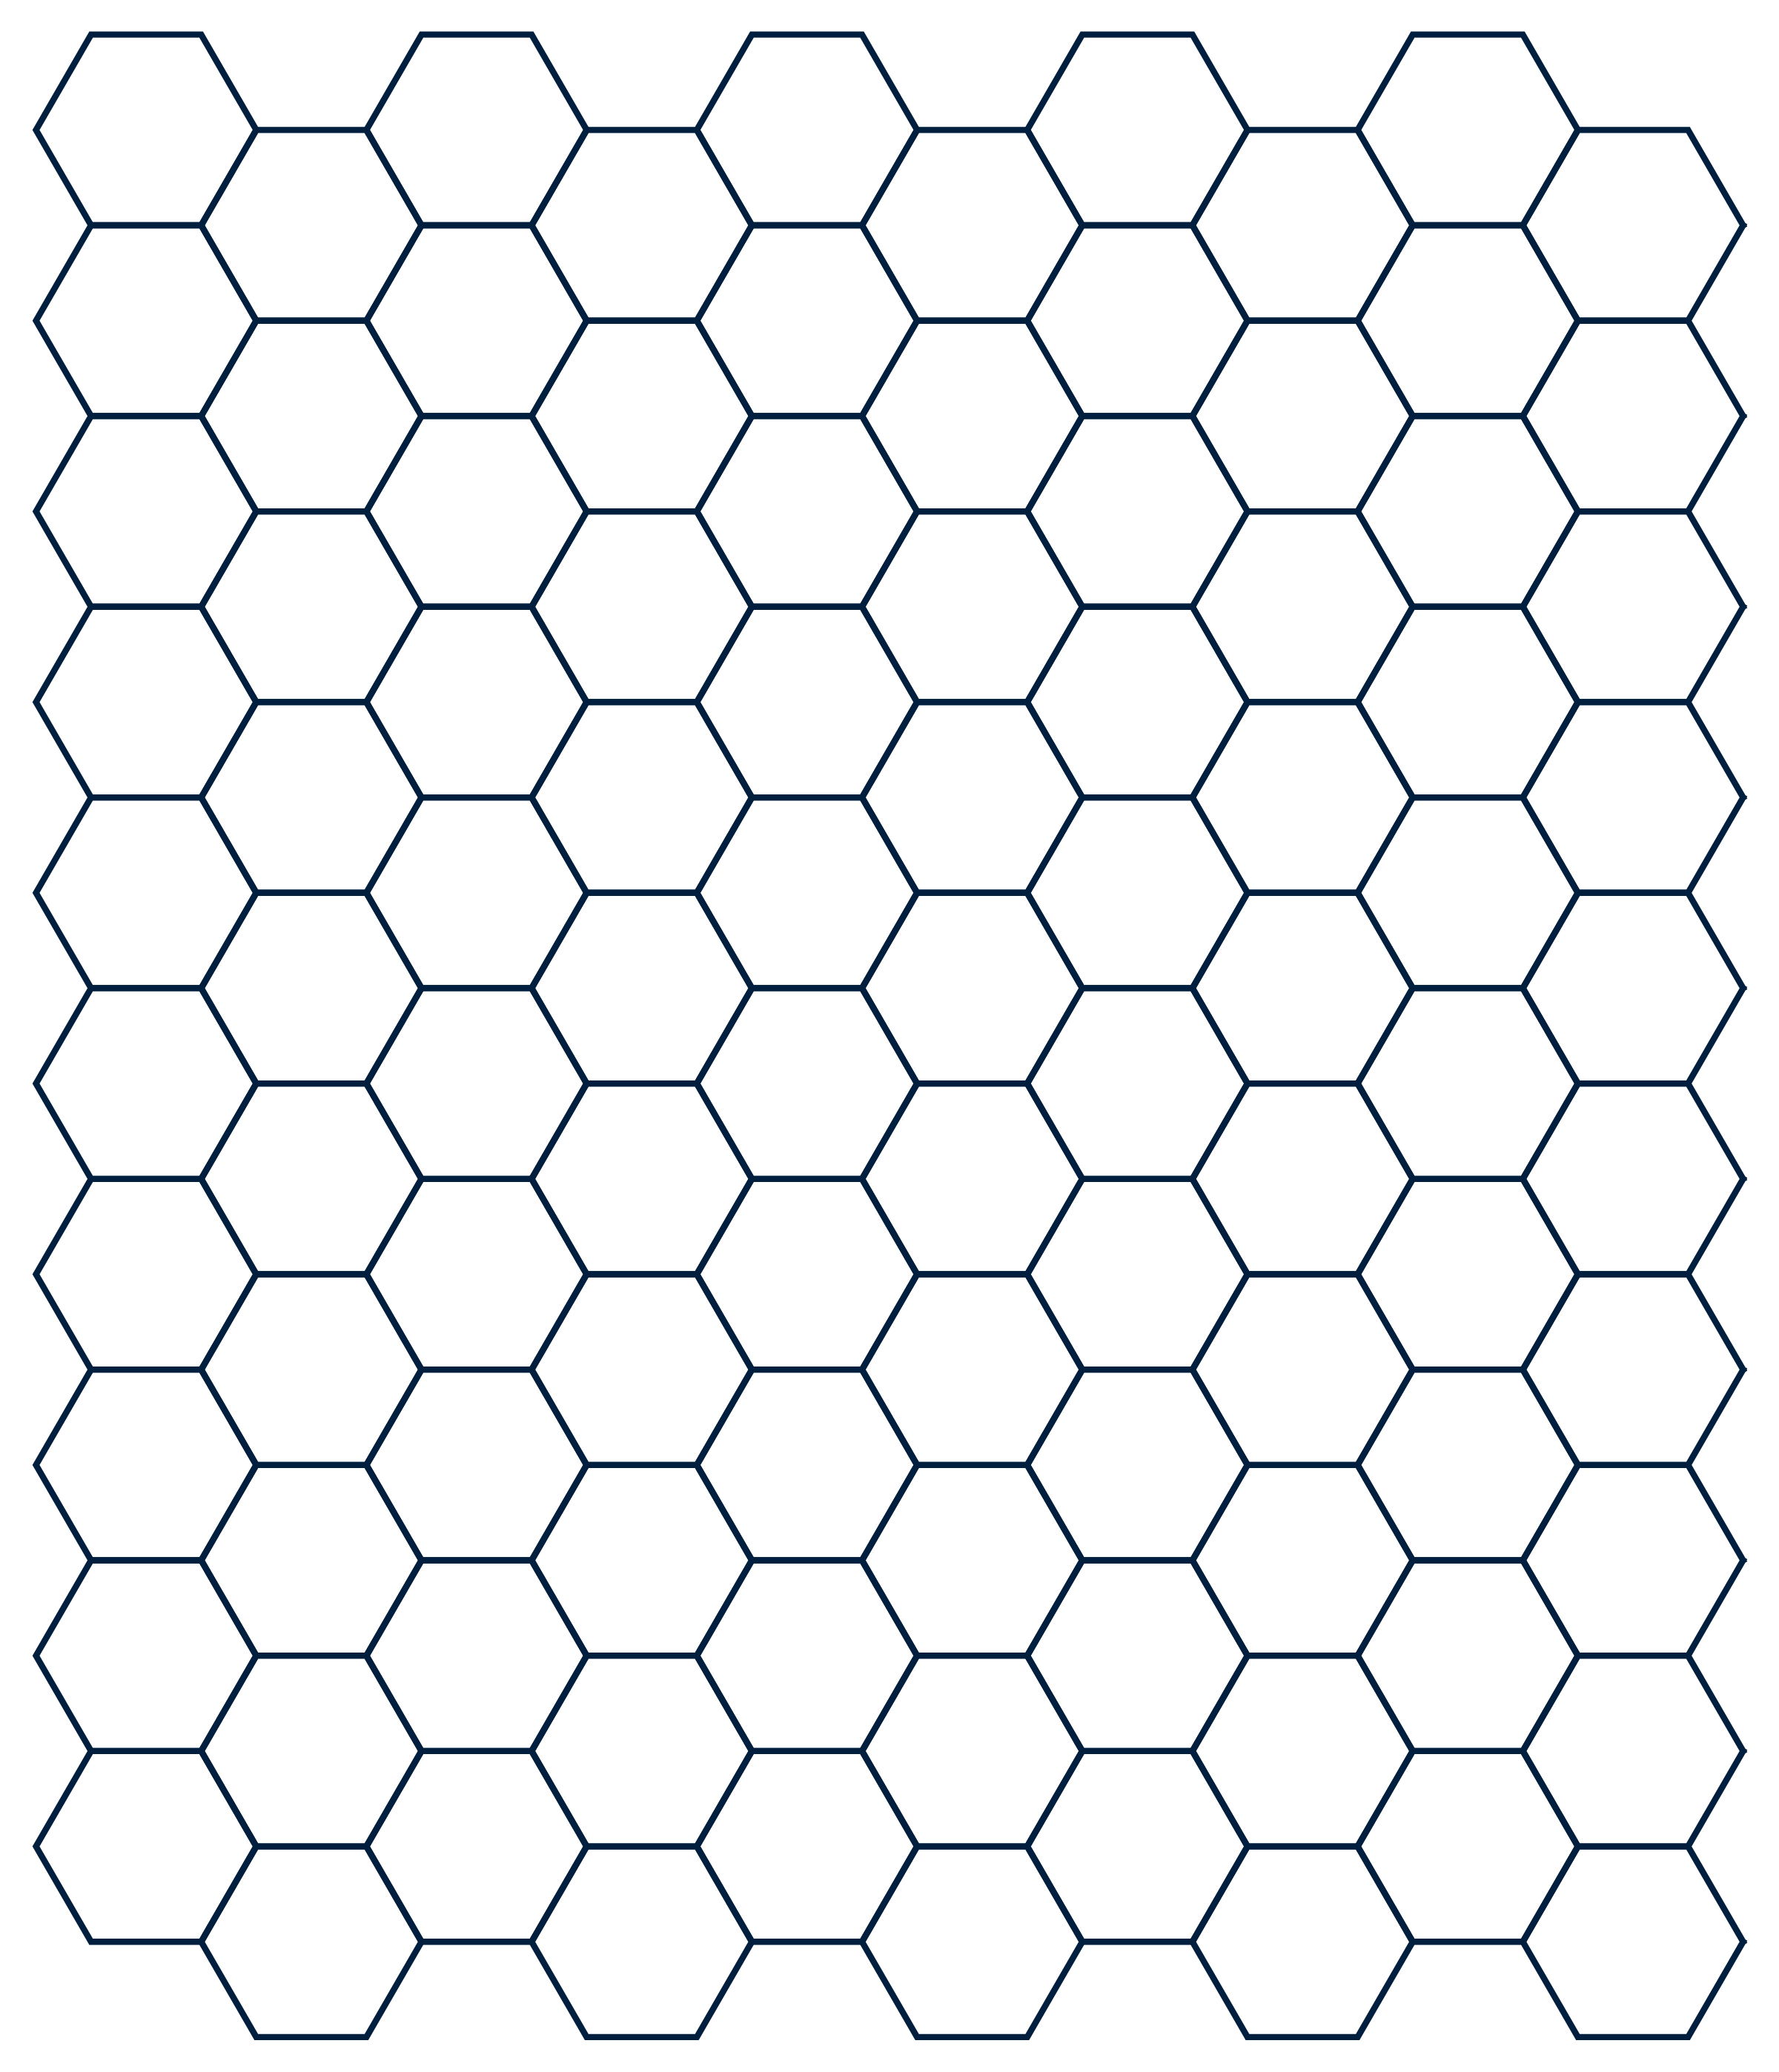
\includegraphics[width=\textwidth]{hexagon}
                \caption{Tiling by hexagons}
                \label{fig:hexagon}
        \end{subfigure}
        \caption[Regular Polygon Tilings]{Regular tiling of the plane using single polygon protosets}\label{fig:regular}
\end{figure}

As we will see, while polygons of 3-, 4-, and 6-fold symmetries, as above, admit plane tilings, 5-fold symmetry is special. In experimenting with plane tilings by regular polygons, Kepler attempted to build tilings from polygons with fivefold symmetry. Pentagons alone will not tile the plane, as the gap between two abutting pentagons will not accommodate another. So, Kepler experimented with packing irregular polygons, see Fig.\ref{fig:Experiments}. One such pattern, Aa, can be continued as a plane tiling, Fig.\ref{fig:tilingmonsters}. However, the Aa pattern made use of pentagons, pentagrams, decagons, and another polygon formed by `fusing' two decagons. Kepler called such fused decagons monsters. 

As we will see in the discovery of aperiodic tilings, five is a troublesome notion in plane tilings, whether pentagon tiles or global five-fold symmetry. However, unlike Kepler's monsters, we will see that such tilings do not damage the theory of plane tilings, but deeply enrich it.

\begin{figure}[H]
        \centering
        \begin{subfigure}[b]{0.9\textwidth}
                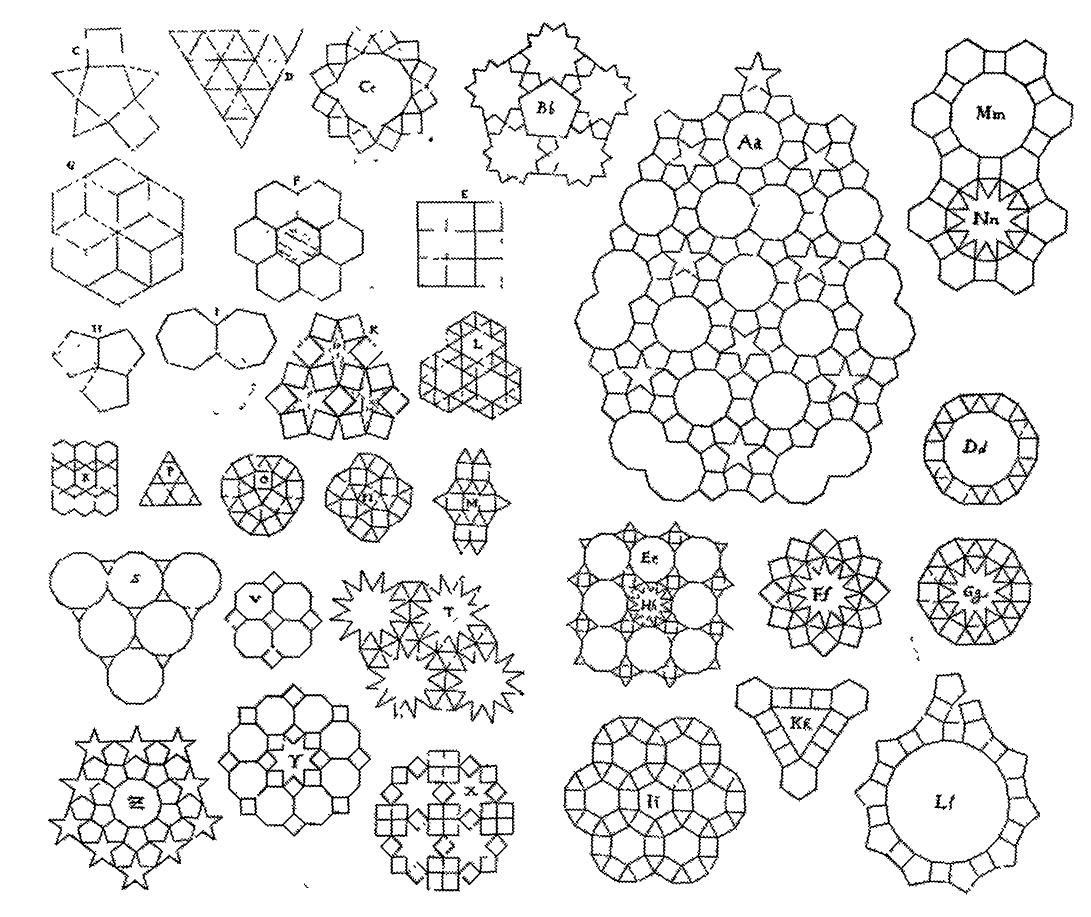
\includegraphics[width=\textwidth]{KeplersExperiments}
                \caption{Kepler's Experiments with Polygon Packing. \cite{Senechal1996}}
                \label{fig:Experiments}
        \end{subfigure}
        
        ~ %add desired spacing between images, e. g. ~, \quad, \qquad, \hfill etc.
          %(or a blank line to force the subfigure onto a new line)
        \begin{subfigure}[b]{0.9\textwidth}
                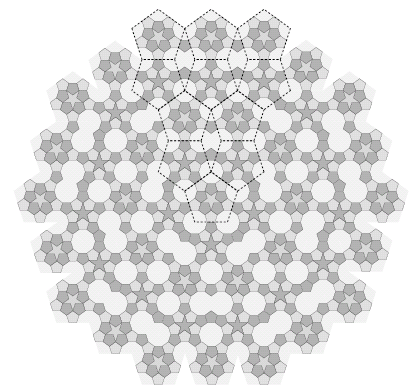
\includegraphics[width=\textwidth]{Monsters}
                \caption{The Aa pattern from above can be continued to tile the plane. However, to do so, Kepler employed `fused' decagons, which he called monsters. We can see that these monsters result from filling the gaps in a regular pentagon tiling. \cite{CraigKaplan}}
                \label{fig:tilingmonsters}
        \end{subfigure}\hfill
         \caption[Kepler's Experiments with Monsters]{Kepler's experiments with polygon packing produced a tiling of the plane by pentagons, pentagrams, decagons, and fused decagons, which Kepler called monsters.}
         \label{fig:Monsters}
\end{figure}

\section{Discovering Aperiodic Tessellations} %DONE
Studied in the mid-1900's was a class of tilings produced by spiraling deformed isosceles triangles about a central point. A method discovered by Micheal Goldberg in 1955 generates these spiral tilings readily. Further, due to their spiraling arrangement, these tilings admit no translational symmetries, so non-periodic. However, these spiral tilings are admitted by protosets which also admits periodic tilings. In fact, all other non-periodic tilings known at the time, also notably Golomb's `reptiles', were formed from protosets which also admit periodic tilings.

\begin{figure}
\begin{subfigure}{0.4\textwidth}
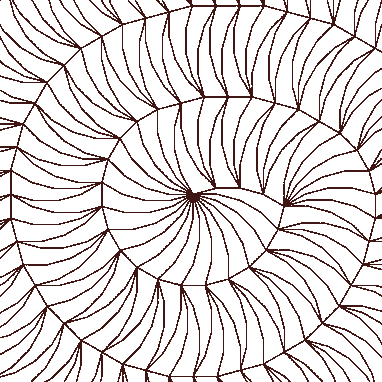
\includegraphics[width=\textwidth]{monohedral}
\end{subfigure}\hfill
\begin{subfigure}{0.4\textwidth}
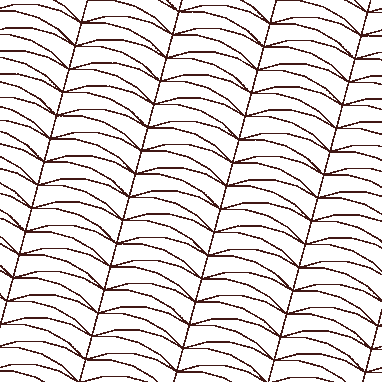
\includegraphics[width=\textwidth]{monohedral-trans}
\end{subfigure}
\caption[Spiral Protosets also admit Periodic Tilings]{Spiral tilings are non-periodic, but their protosets also admit periodic tilings \cite{Austin2007}.}
\end{figure}

It was conjectured that no protosets existed which allow only non-periodic tiling. That is, that no aperiodic protosets were possible. This was proved untrue when, in 1961, Hao Wang began writing on protosets composed of unit squares with coloured edges, called Wang dominoes. The matching rules for these dominoes require adjacent dominoes to share the same colour on their abutting edge, with rotation and reflection of the prototiles not allowed. Wang was concerned with questions in logic, specifically investigating algorithmic procedures for deciding whether any arbitrary set of dominoes would admit a plane tiling, called decision procedures. Wang posed a conjecture that any protoset which can admit a plane tiling will also admit a periodic tiling, and Wang showed that if this is true then there must also be an algorithmic procedure for deciding whether such a set will tile. 

In 1964, Robert Berger showed in his doctoral thesis from Harvard University that Wang's conjecture is false, that there is no algorithmic decision procedure for the tiling ability of any arbitrary protoset. The implication of Berger's work is that there must be an aperiodic protoset of Wang dominoes. Further, Berger constructed such a protoset, using 20,426 dominoes. In his later work, Berger produced a smaller protoset, requiring only 104 dominoes. Donald Knuth further reduced this number by finding an aperiodic Wang protoset of only 92 tiles.

As discussed previously, tiling matching rules can be realized by deformations on the edges of the prototiles. For instance, instead of the coloured edges of the Wang dominoes, consider deforming the edges of the squares into protrusions and cavities, producing prototiles like pieces of a jigsaw puzzle. These deformations can be chosen in such a way that they permit only the same arrangements as did the coloured edges of the dominoes, however, this representation also allows for rotation and reflection of the prototiles, previously not considered by Wang. 

By representing the protoset as described above, in 1971 Raphael Robinson constructed an aperiodic protoset requiring only six prototiles. The prototiles used by Robinson are considered to still be in the category of `square' tiles, and whether size of an aperiodic protoset of square tiles can be reduced to fewer than six tiles is still unknown. However, it is conjectured that six is the minimum number of square tiles to produce an aperiodic protoset. This was supported in 1977 when Robert Ammann found a different aperiodic protoset of six square prototiles.

In 1973, Roger Penrose found an aperiodic protoset of six, non-square tiles.  Penrose continued this process of reduction and, in 1971, reduced the size of his aperiodic protoset to four tiles, and shortly after reduced them further to two tiles. There are arbitrarily many representations of these two prototiles, but two representations are considered simplest and most recognizable. 

The first of these representations, the Penrose Rhombs, is a set of two rhombi with equal lengths, but different internal angles (See Fig.\ref{fig:Rhombs}). The thin rhombus, \textbf{t}, has corner angles of $\frac{\pi}{5}$ and $\frac{4 \pi}{5}$ (or $36 \degree$ and $144 \degree$). The thick rhombus, \textbf{T}, has corner angles  $\frac{2 \pi}{5}$ and $\frac{3 \pi}{5}$ (or $72 \degree$ and $108 \degree$). Both thin and thick rhombi can be produced by the composition of Robinson's Golden triangles, named for Robinson's 1975 notes on their construction. The rhombs can be produced by reflecting the isosceles Robinson triangles across their bases. The ratio of the leg and base lengths in the Robinson triangles is the Golden Ratio, \textbf{ $\phi= \frac{1+\sqrt{5}}{2}\approx 1.6180$}. This ratio will appear repeatedly throughout this discussion of Penrose tilings. 

The other common representation of Penrose's tiles is the Kite and Dart protoset, named by John Conway. These prototiles are also produced by the composition of Robinson triangles, rather by reflection across their legs. 

Neither the Rhombs nor the Kites and Darts tilings were publicized until after Penrose filed for patents on the shapes, due to their commercial potential as board game puzzles. It was Martin Gardner who finally published Penrose and Conway's work on describing these tilings, as well as their method of constructing the tiling by substitution, in his 1977 ``Mathematical Games'' column in \textit{Scientific American}. 

In 1981, Dutch mathematician Nicolaas de Bruijn provided other methods of constructing the Penrose tiling, by projecting of five-dimensional cubic structure and also by infinite paths on directed graphs, which will discussed later. De Bruijn also showed the relationship between the Penrose tiling and five families of parallel lines, called the Pentagrid. De Bruijn's work represents the characterization of Penrose tilings as algebraic objects, and offers deep insight into their nature. 

The practical importance of these theories on aperiodic tiling was realized in the 1980's with the discovery by materials scientist Dan Shechtman of certain aluminum-manganese alloys which produce crystallographic diffraction patterns with no translational symmetries. Shechtman was awarded the 2011 Nobel Prize in Chemistry for his discovery of these structures, known now as quasicrystals. In 2009, the first natural quasicrystal was discovered, the mineral icosahedrite, whose diffraction pattern displays fivefold symmetry previously thought impossible in crystalline structures. This past month, in March 2015, the second natural quasicrystal was discovered in a meteorite, with a diffraction pattern displaying decagonal symmetry \cite{Bindi2015}. Marjorie Senechal formalizes the relationship between aperiodic tiling and the geometry of quasicrystals in her 1995 monograph \textit{Quasicrystals and Geometry}. 


\chapter{Substitution Construction}

\section{Rhombs Representation of the Penrose Tiling} %DONE
As introduced, there are multiple protoset representations that admit the Penrose tiling. However, the construction methods outlined in this section were described initially by de Bruijn, who favoured the Rhombs representation.  For this reason, we will consider only construction of the Penrose tiling by the Rhombs protoset (see Fig.\ref{fig:Rhombs}). 

Since this protoset is composed of two rhombi, it might be suspected that the prototiles can be arranged to produce a periodic tiling, since rhombi can generally produce periodic tilings. Consider, for example, the tiling produced by adjacent rows of thick and thin rhombi (see Fig.\ref{fig:RhombsPeriodic}). This tiling underscores the necessity of edge-matching rules for the aperiodic protoset. 

The edge-matching rules of the Penrose rhombs have been illustrated with blue and orange curves in Fig.\ref{fig:Rhombs}. If two tiles are adjacent in a tiling, then curves of the same colour must meet along the abutting edge. For example, the previously discussed periodic rhombus tiling is not permitted given this edge-matching criteria, because these curves do not meet along adjacent tiles (see Fig.\ref{fig:RhombsPeriodicRules}). Further, recall from previous description that matching criteria can be realized through prototile edge deformations (see Fig.\ref{fig:deformedchecker}). This allows us to consider the Rhombs protoset with matching rules as distinct from the Rhombs without matching rules, permitting us to describe the former as aperiodic. 


\begin{figure}[H]
\begin{subfigure}[t]{0.4\textwidth}
\centering
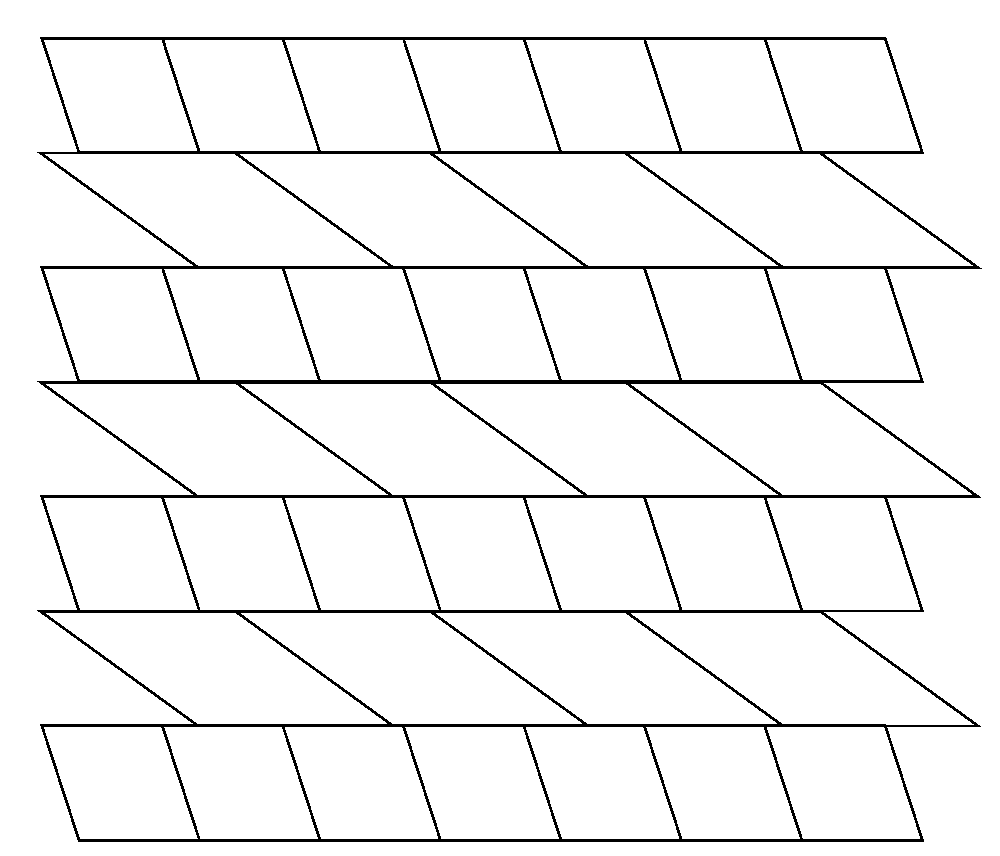
\includegraphics[width=\textwidth]{RhombPeriodic}
\caption{Periodic tiling of thin and thick rhombi, admitted in the absence of edge-matching rules.}
\label{fig:RhombsPeriodic}
\end{subfigure}\hfill
\begin{subfigure}[t]{0.4\textwidth}
\centering
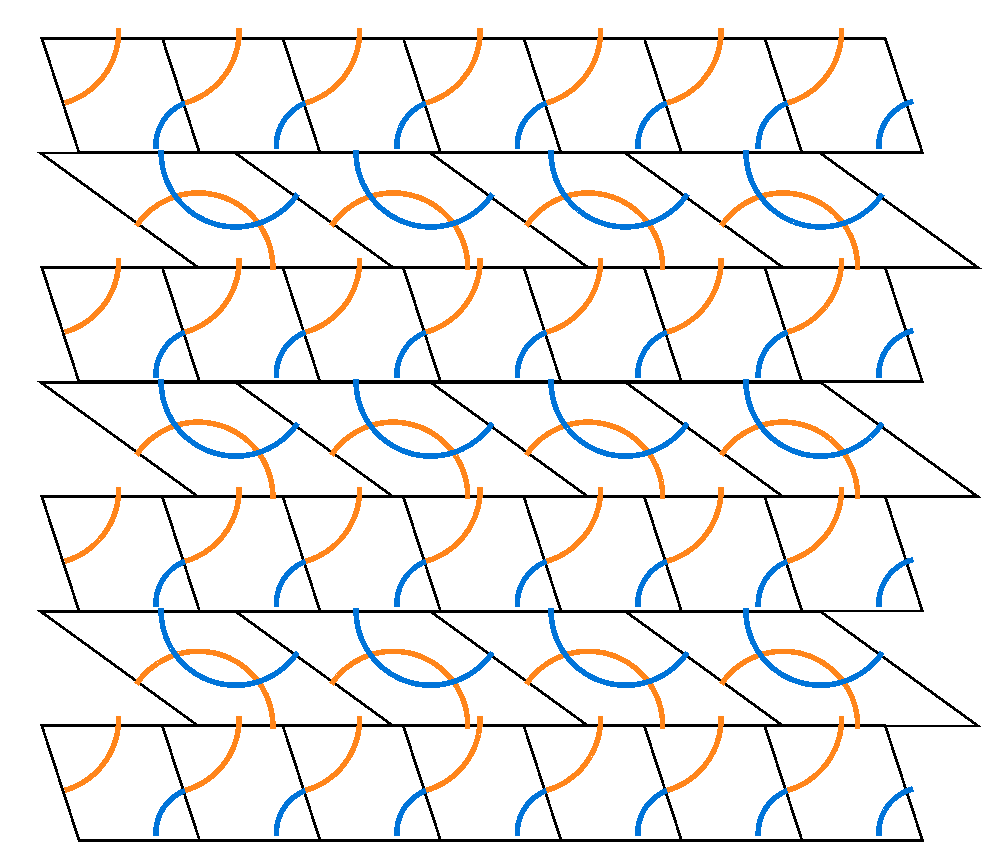
\includegraphics[width=\textwidth]{RhombPeriodicRules}
\caption{Matching rules require blue and orange curves to meet along adjacent edges. Clearly, this tiling does not satisfy these matching rules.}
\label{fig:RhombsPeriodicRules}
\end{subfigure}
\caption[Rhomb Matching Rules Forcing Aperiodicity]{Periodic tiling using Penrose rhombs is only possible in the absence of edge-matching rules.}

\end{figure}

\begin{figure}
        \centering
        \begin{subfigure}[b]{\textwidth}
        \begin{subfigure}[b]{0.5\textwidth}
                \centering
                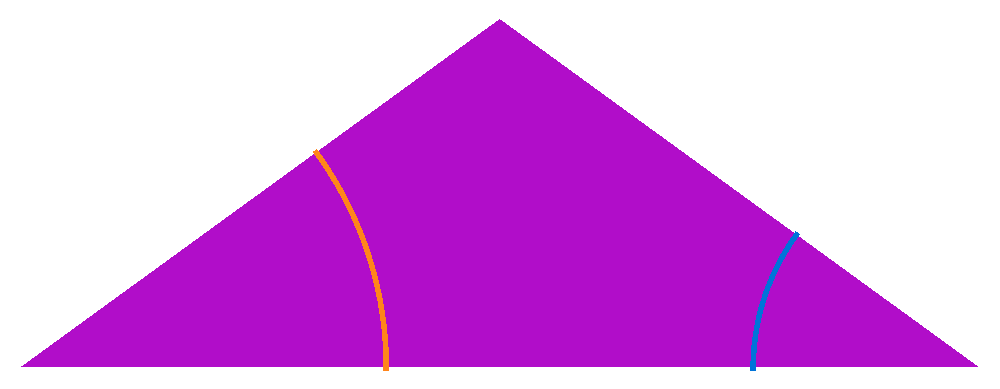
\includegraphics[scale=0.5]{RobinsonFat}
                \subcaption{Thick Robinson Triangle}
                \label{fig:RobThick}
        \end{subfigure}\hfill%
        ~ %add desired spacing between images, e. g. ~, \quad, \qquad, \hfill etc.
          %(or a blank line to force the subfigure onto a new line)
        \begin{subfigure}[b]{0.5\textwidth}
                \centering
                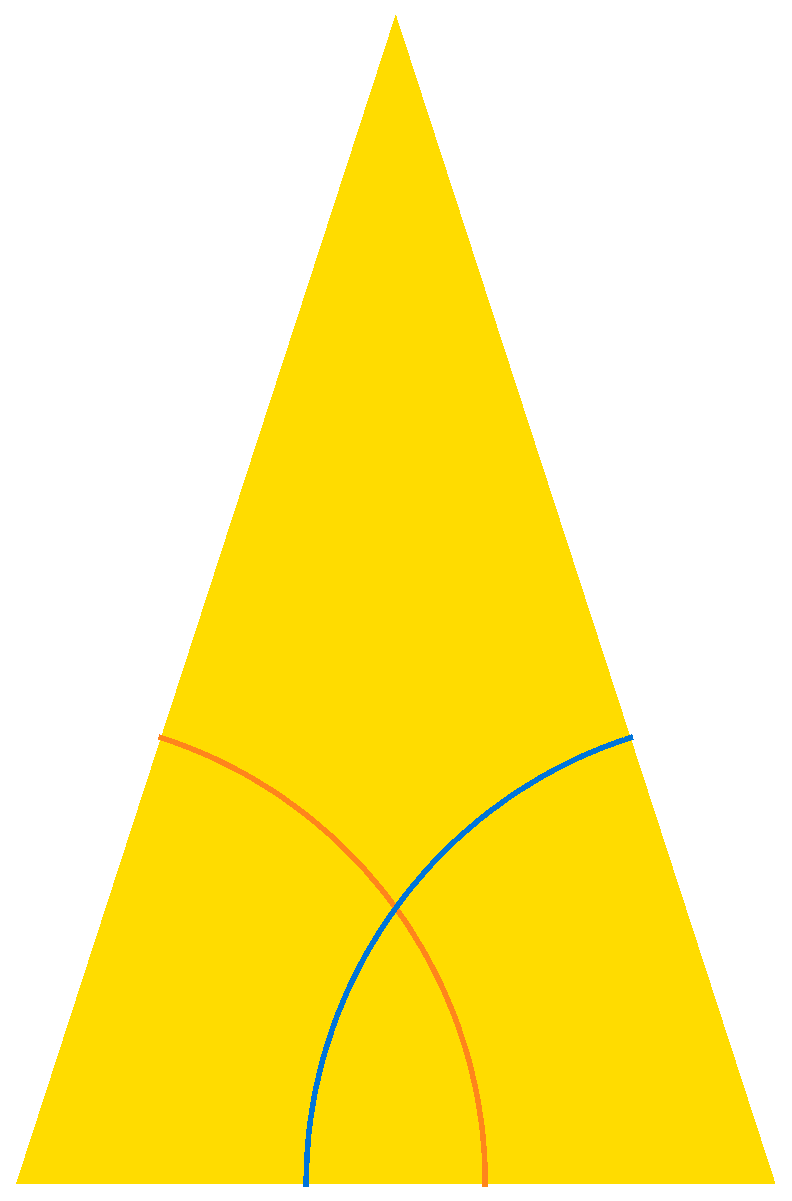
\includegraphics[scale=0.3]{RobinsonSkinny}
                \subcaption{Thin Robinson Triangle}
                \label{fig:RobThin}
        \end{subfigure}
        \caption*{Robinson Triangles with Golden leg-to-base ratio, $\phi$.}
        \label{fig:RobTris}
        \end{subfigure}
        ~ %add desired spacing between images, e. g. ~, \quad, \qquad, \hfill etc.
          %(or a blank line to force the subfigure onto a new line)
          
        \begin{subfigure}[b]{\textwidth}
        \begin{subfigure}[b]{0.5\textwidth}
        \centering
                \raisebox{40px}{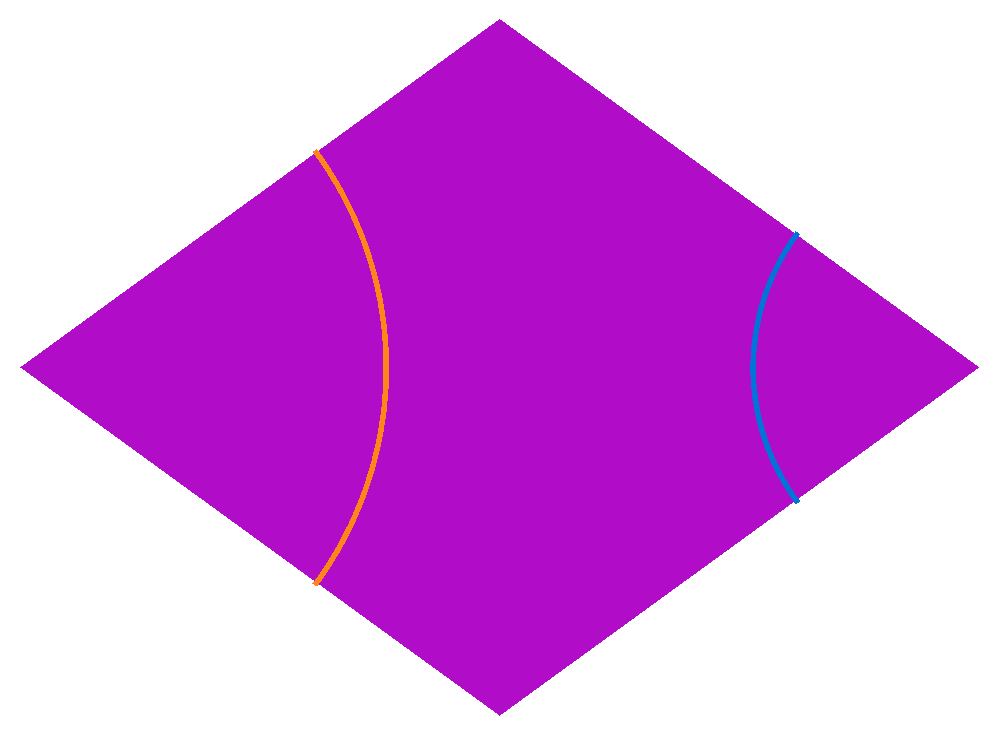
\includegraphics[scale=0.5]{RhombFat}}
                \caption{Thick Penrose Rhomb}
                \label{fig:ThickRhomb}
        \end{subfigure}\hfill
        \begin{subfigure}[b]{0.5\textwidth}
        \centering
                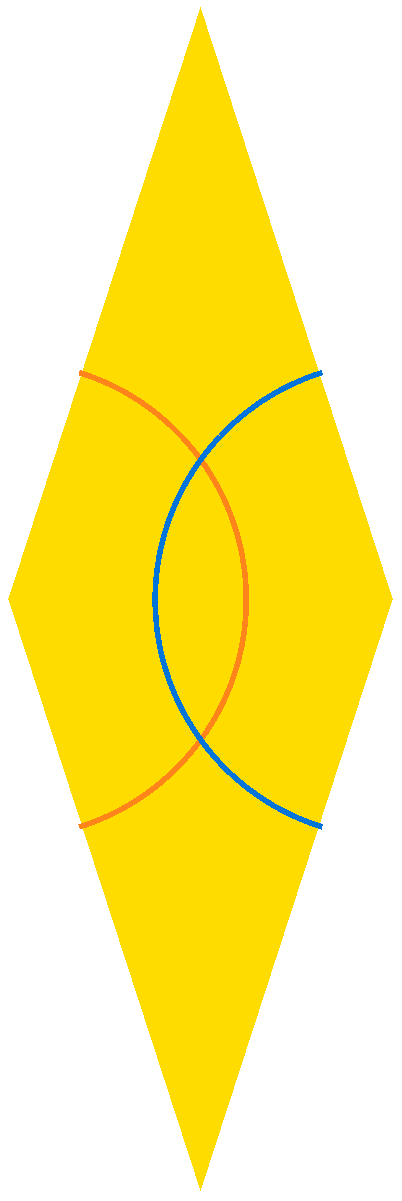
\includegraphics[scale=0.6]{RhombSkinny}
                \caption{Thin Penrose Rhomb}
                \label{fig:ThinRhomb}
        \end{subfigure}   
                \caption*{ \centering Penrose Rhombs from Robinson triangles. Blue and Orange curves illustrate matching rules.}
                \label{fig:JustRhombs}     
        \end{subfigure}
        \caption[Robinson Triangles and Penrose Rhombs]{Penrose Rhombs are generated by reflecting the Robinson triangles across their bases. The Rhombs with an edge-matching criterion, illustrated by the blue and orange curves, form an aperiodic protoset.}
        \label{fig:Rhombs}
\end{figure}

Now that we have seen the Penrose rhombs protoset, and the criteria which allow two tiles to meet, we can investigate how to construct valid tilings. 


\section{Non-Local Growth} %DONE
Penrose tilings cannot be procedurally constructed one-tile-at-a-time, as one would tile a floor. In attempting to construct a tiling this way, there is no guarantee that any finite, valid arrangement of tiles can be continued infinitely. 

When we construct a tiling one-tile-at-a-time, rarely are our next tile placements forced. Usually, we have the option to choose the next tile from among both thick and thin Rhombs. One might anticipate that as long as we choose our tile arrangements such that we satisfy the local matching rules, we will eventually tile the entire plane. However, it is in these choices that we encounter a problem with this one-at-a-time method, we can choose incorrectly. If we place our tiles one-at-a-time we can make mistakes.

\begin{mydef}
A \textbf{mistake} is a valid placement of a tile which causes the resulting tiling to not continue infinitely to tile the plane. The manifestation of this mistake, either as an unfillable gap or overlap, is called an \textbf{error}. \cite{Penrose1989,Ross}
\end{mydef}

For example, consider the arrangement of tiles in Fig.\ref{fig:mistake}. As we can see from the blue and orange circle arcs, these tiles are validly arranged under the edge matching rules. However, despite the validity of this arrangement, this is a mistake. The error of this mistake manifests itself immediate, we have created an gap which cannot be filled by any valid tile arrangement. One might think that we could fill this gap with a thin Rhomb, as seen in Fig.\ref{fig:error}, but we see that such an arrangement does not satisfy the edge matching rules.

\begin{figure}[h]
\centering
\begin{subfigure}{0.6\textwidth}
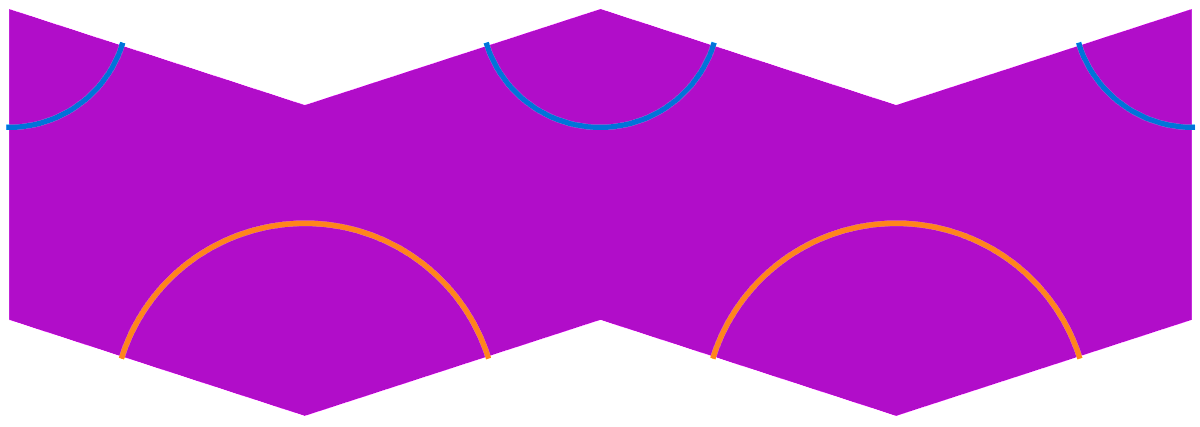
\includegraphics[width=\textwidth]{Mistake}
\caption{Although valid, this arrangement of thick Rhombs is a mistake.}
\label{fig:mistake}
\end{subfigure}\\
\begin{subfigure}{0.6\textwidth}
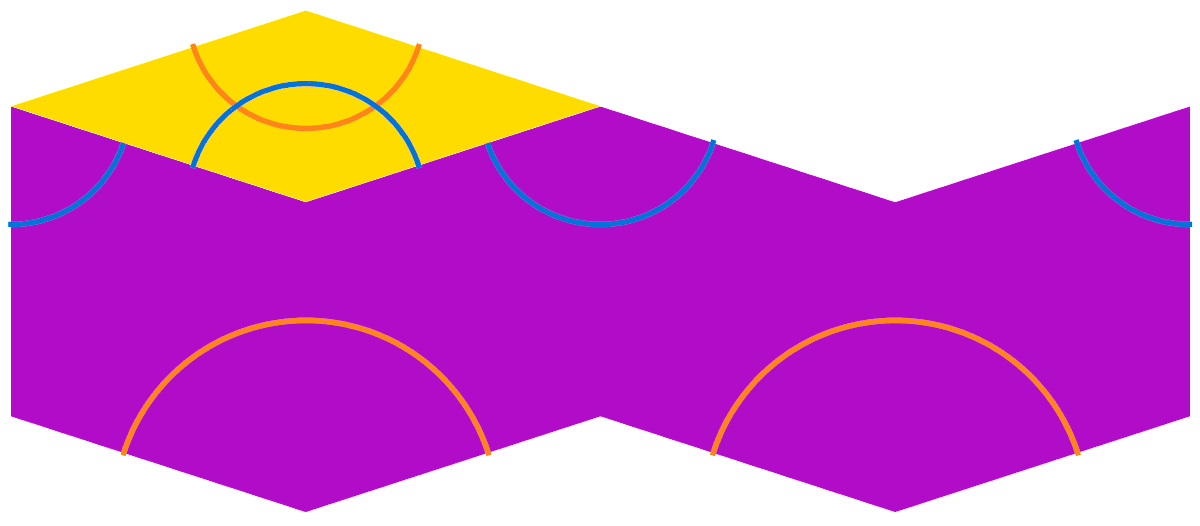
\includegraphics[width=\textwidth]{MistakeNext}
\caption{The manifestation of this mistake, the error, is this gap no valid arrangement could fill.}
\label{fig:error}
\end{subfigure}
\caption[A Simple Mistake]{A simple mistake results in an error which cannot be continued to produce a valid tiling of the whole plane.}
\label{fig:mistakes}
\end{figure}

However, mistakes are often far more sinister than the one illustrated in Fig.\ref{fig:mistakes}. Here we see a mistake that manifested its error immediately. That is, the error occurs adjacent to the mistake. This is not true in general. As we will see shortly, Penrose tilings must satisfy certain substitution criteria. One effect of satisfying these substitution criteria is that Penrose tilings will have structures that must agree across arbitrarily large distances. What does this mean for a one-tile-at-a-time construction method? Well, it means that the placement of a tile could be a mistake due to the placement of another tile arbitrarily far away. What's even worse? This mistake may not manifest its error for another arbitrarily large distance from either tile placements. This means that if we were trying to tile the plane one-tile-at-a-time, we could generate a mistake because of the placement of another piece arbitrarily far away from the piece we're placing, and we wouldn't even know about our mistake until arbitrarily many other pieces have been placed. This is because Penrose tilings are non-local. That is, while the matching rules describe local conditions, the substitution hierarchy we will soon discuss imposes global conditions on the tiling. Non-locality of the Penrose tiling, in short, means that the placement of tiles must globally agree with the tiling, so arrangements cannot be determined by local matching rules. For this reason, we cannot procedurally tile the Penrose tiling one-tile-at-a-time.


\section{Deflation and Inflation} %DONE
Despite non-locality, Penrose and Conway showed that we can construct arbitrarily large tilings by repeated application of substitution rules.

To clearly understand the substitution rules on the rhombs, we will first demonstrate the substitution of the constituent Robinson triangles (Fig.\ref{fig:RobSubs})

\begin{figure}[H]
        \centering
        \begin{subfigure}[t]{\textwidth}
        \begin{subfigure}[t]{0.4\textwidth}
                \centering
               \raisebox{9px}{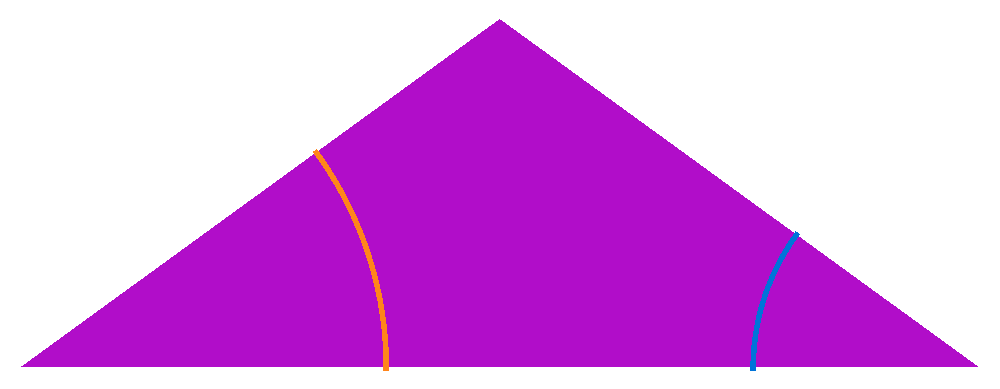
\includegraphics[scale=0.4]{RobinsonFat}}
        \end{subfigure}\hfill \raisebox{30px}{\huge$\rightarrow$} \hfill%
        ~ %add desired spacing between images, e. g. ~, \quad, \qquad, \hfill etc.
          %(or a blank line to force the subfigure onto a new line)
        \begin{subfigure}[t]{0.4\textwidth}
                \centering
                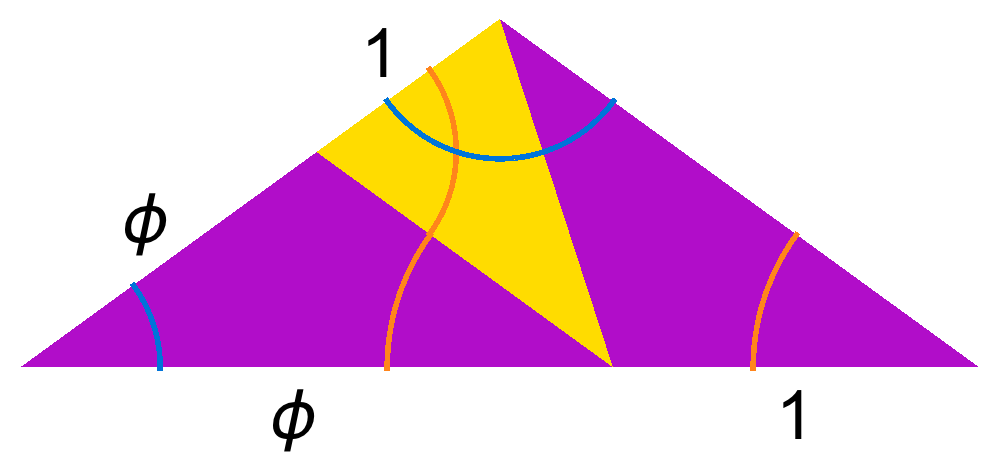
\includegraphics[scale=0.4]{RobFatSub}
        \end{subfigure}
        \caption{Substitution rule for Thick Robinson triangle}
        \label{fig:RobSubThick}
        \end{subfigure}
        ~ %add desired spacing between images, e. g. ~, \quad, \qquad, \hfill etc.
          %(or a blank line to force the subfigure onto a new line)
          
        \begin{subfigure}[b]{\textwidth}
        \begin{subfigure}[b]{0.4\textwidth}
        \centering
		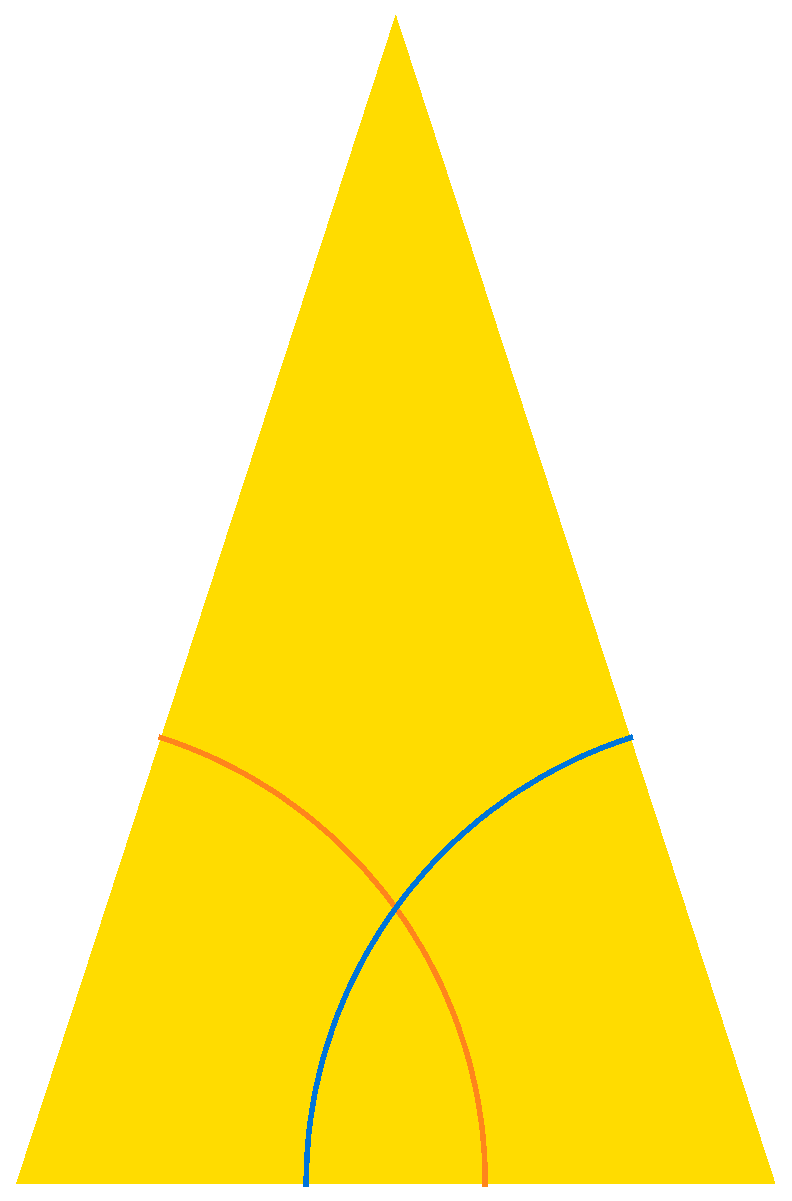
\includegraphics[scale=0.3]{RobinsonSkinny}
        \end{subfigure}\hfill \raisebox{30px}{\huge$\rightarrow$} \hfill
        \begin{subfigure}[b]{0.4\textwidth}
        \centering
                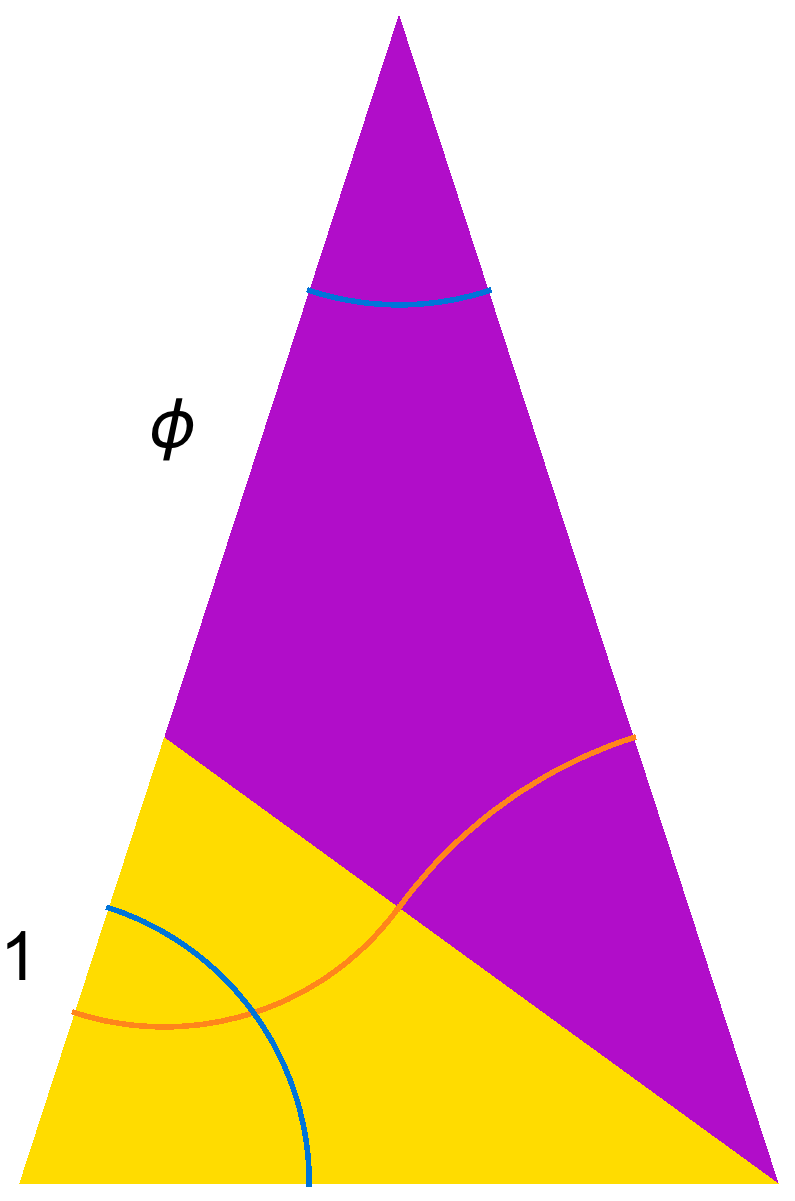
\includegraphics[scale=0.3]{RobSkinnySub}
        \end{subfigure}   
        \caption{Substitution rule for Thick Robinson triangle}
        \label{fig:RobSubThin}
        \end{subfigure}
        \caption[Robinson Triangles Deflation]{Substitution rules demonstrated on Robinson triangles. The substitution fragments each Robinson triangle into Robinson sub-triangles. The vertices of these sub-triangles are given such that the edges of the substituted triangle are divided according to the Golden ratio. The ratios of these divided edges are labeled accordingly. Note that these substitutions produce valid arrangements as per the edge-matching rules, illustrated by the orange and blue curves.}
        \label{fig:RobSubs}
\end{figure}

Recall that these Robinson triangles generate Penrose Rhombs by reflection across their bases (Fig.\ref{fig:Rhombs}). With that in mind, consider the above substitution applied to the Rhombs, such that each constituent Robinson triangle composing the Rhomb undergoes substitution as above. These substitution rules, applied to the Penrose Rhombs, is known as the process of \textbf{deflation}.

\begin{figure}[H]
        \centering
        \begin{subfigure}[t]{\textwidth}
        \begin{subfigure}[t]{0.4\textwidth}
                \centering
               \raisebox{30px}{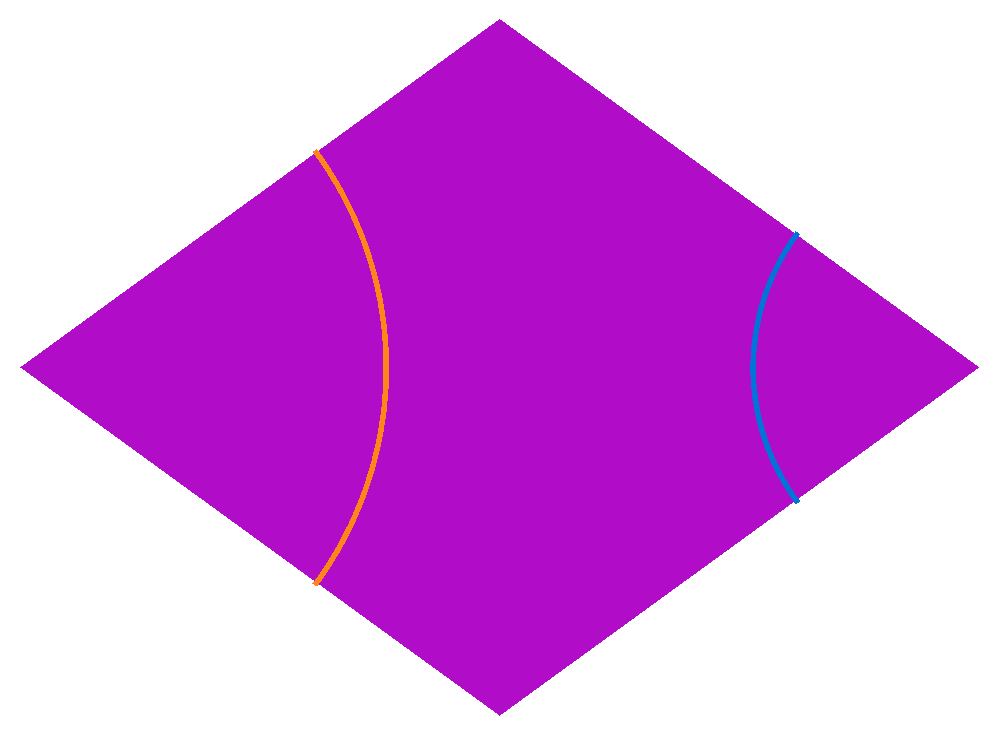
\includegraphics[scale=0.4]{RhombFat}}
        \end{subfigure}\hfill \raisebox{75px}{\huge$\rightarrow$} \hfill%
        ~ %add desired spacing between images, e. g. ~, \quad, \qquad, \hfill etc.
          %(or a blank line to force the subfigure onto a new line)
        \begin{subfigure}[t]{0.4\textwidth}
                \centering
                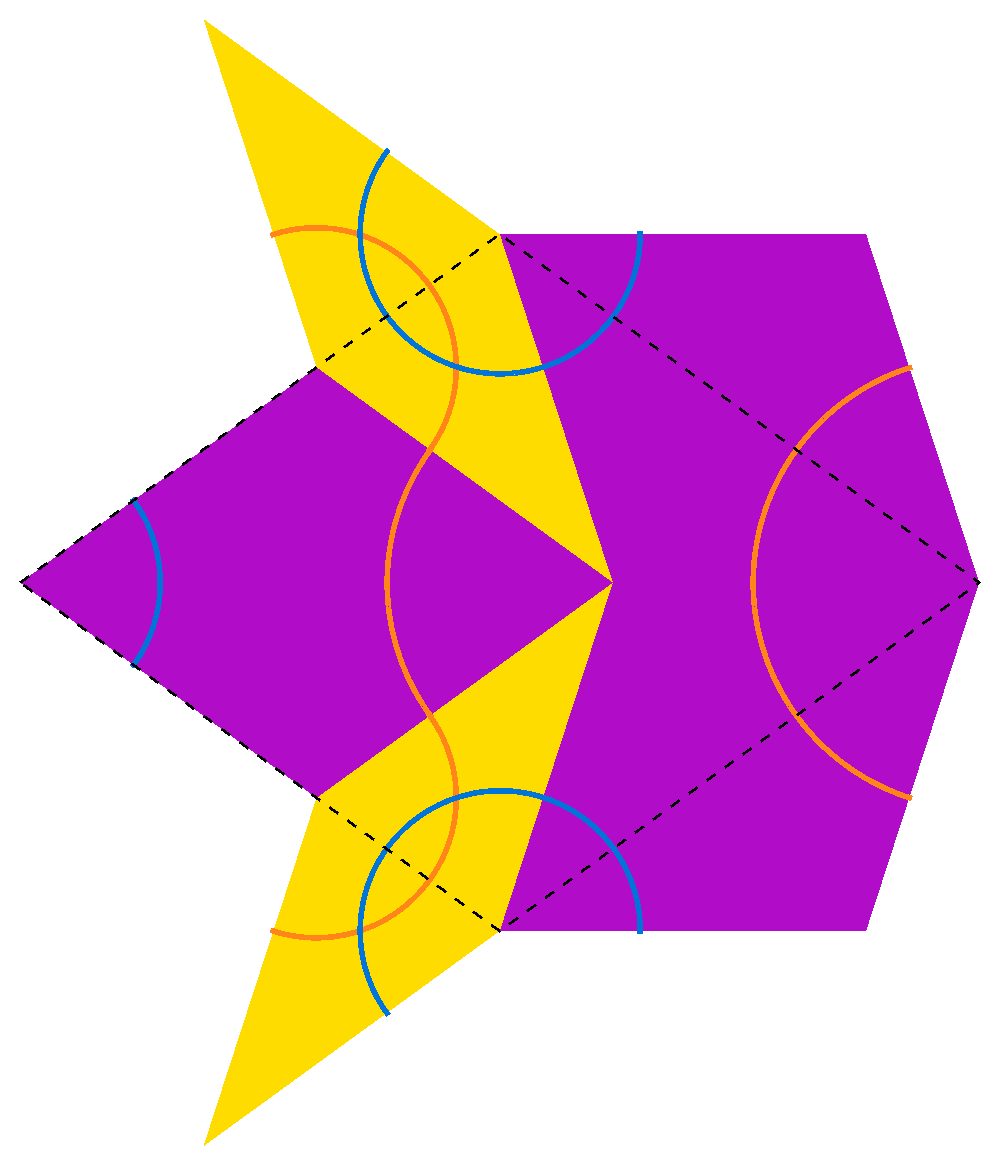
\includegraphics[scale=0.4]{RhombFatSub}
        \end{subfigure}
        \caption{Deflation rule for Thick Penrose Rhomb}
        \label{fig:RhombSubThick}
        \end{subfigure}
        ~ %add desired spacing between images, e. g. ~, \quad, \qquad, \hfill etc.
          %(or a blank line to force the subfigure onto a new line)
          
        \begin{subfigure}[b]{\textwidth}
        \begin{subfigure}[b]{0.4\textwidth}
        \centering
		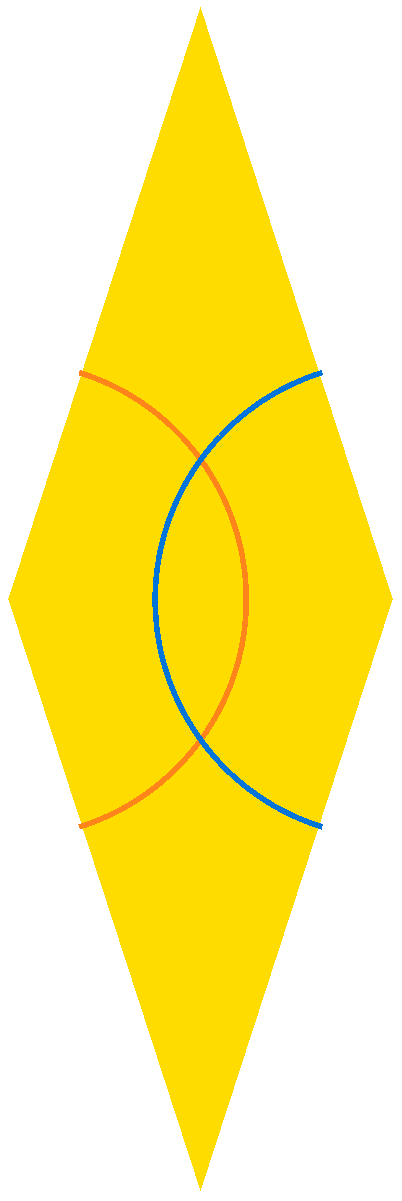
\includegraphics[scale=0.4]{RhombSkinny}
        \end{subfigure}\hfill \raisebox{75px}{\huge$\rightarrow$} \hfill
        \begin{subfigure}[b]{0.4\textwidth}
        \centering
                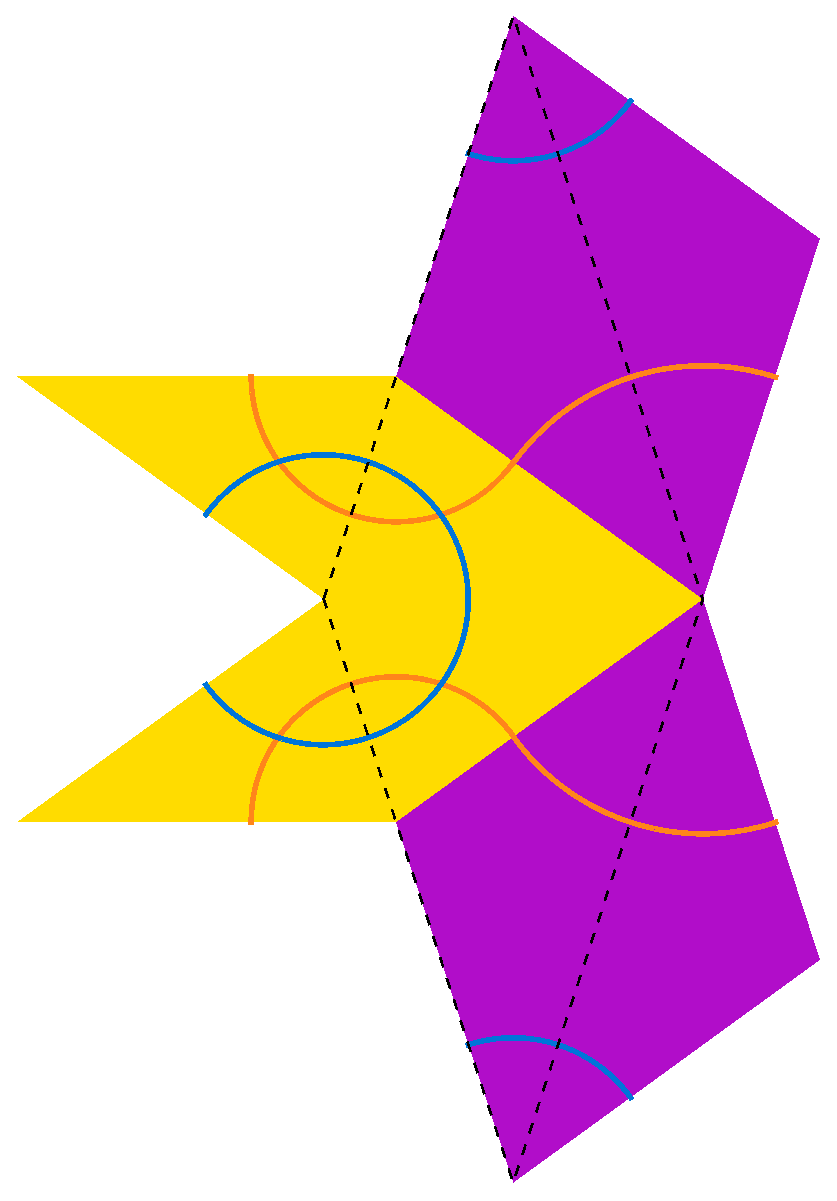
\includegraphics[scale=0.4]{RhombSkinnySub}
        \end{subfigure}   
        \caption{Deflation rule for Thin Penrose Rhomb}
        \label{fig:RhombSubThin}
        \end{subfigure}
        \caption[Penrose Rhombs Deflation]{Deflation rules of the Penrose Rhombs. Pre-substituted rhomb is illustrated with dashed black lines. Note that these substitutions produce valid arrangements as per the edge-matching rules, illustrated by the orange and blue curves.}
        \label{fig:RhombSubs}
\end{figure}

This substitution process can be used to generate arbitrarily large Penrose tilings through a complementary process, called \textbf{inflation}. Following a series of deflation substitutions, the generated tiling is then `inflated' such that the deflated rhombuses are scaled to the same size as the original, pre-deflated rhombuses. Notice that a single application of the deflation rule scales the composite rhombi by a factor of $\frac{1}{\phi}$. This means that, after $n$ iterations of the deflation process, the resulting rhombs can be scaled, or inflated, by a factor of $\phi^n$ to return them to the original rhombus size. We can see in Figures \ref{fig:ThickDeflate} and \ref{fig:ThinDeflate} that iterations of the deflation process produce increasingly complex patterns. 

\begin{figure}[H]
\centering
\begin{tabular}{cc}
	        \begin{subfigure}[b]{0.4\textwidth}
	        \centering
	        \raisebox{30px}{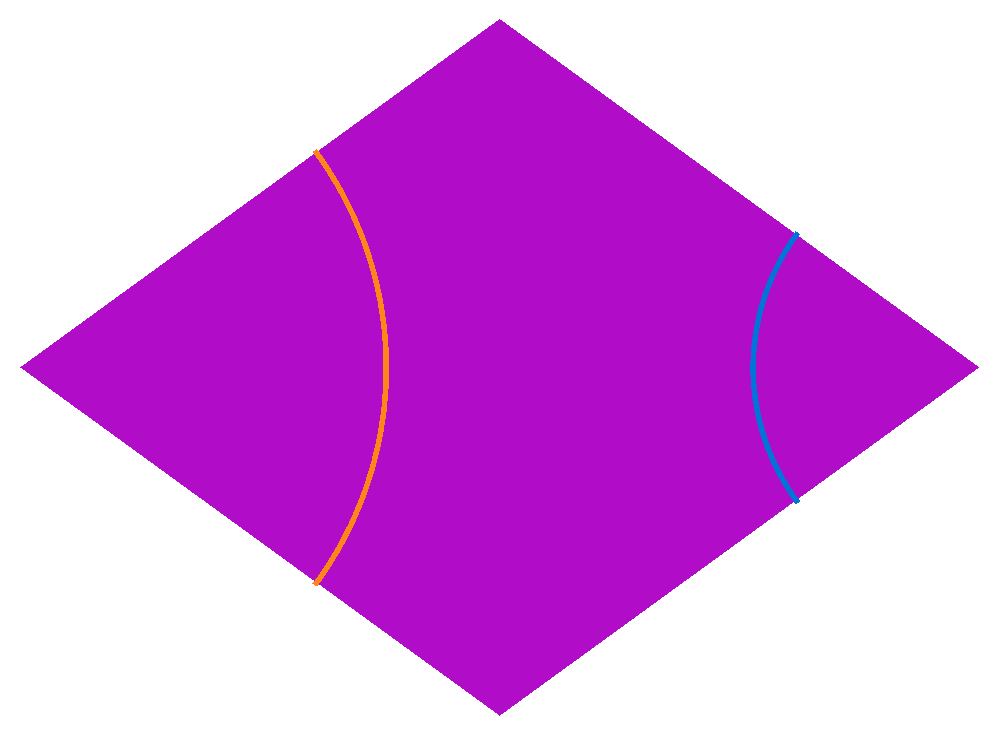
\includegraphics[scale=0.4]{FatInflation0}}
	        \end{subfigure}   &
            \begin{subfigure}[b]{0.4\textwidth}
             \centering
             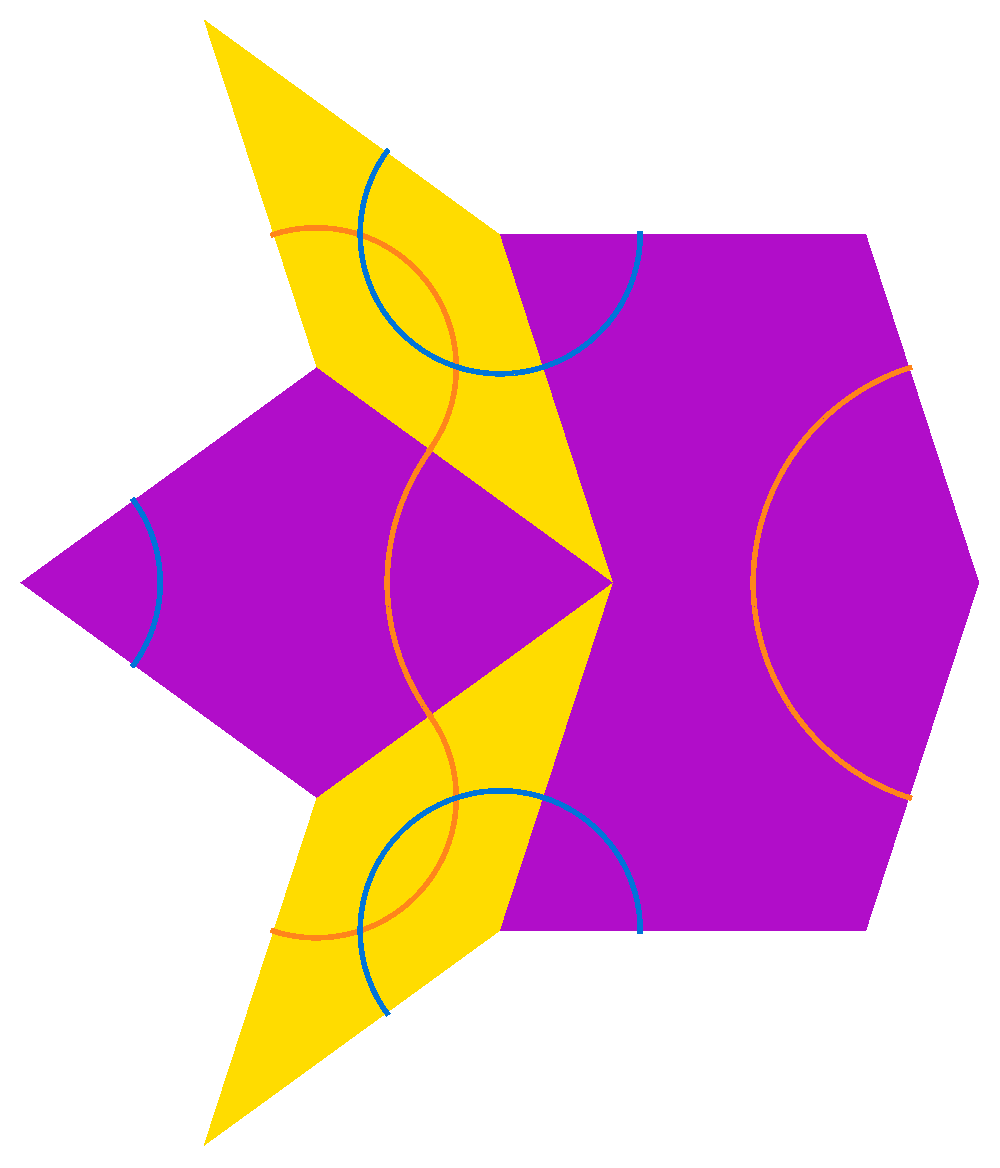
\includegraphics[scale=0.4]{FatInflation1}
             \end{subfigure}   \\
	       	 \begin{subfigure}[b]{0.4\textwidth}
             \centering
             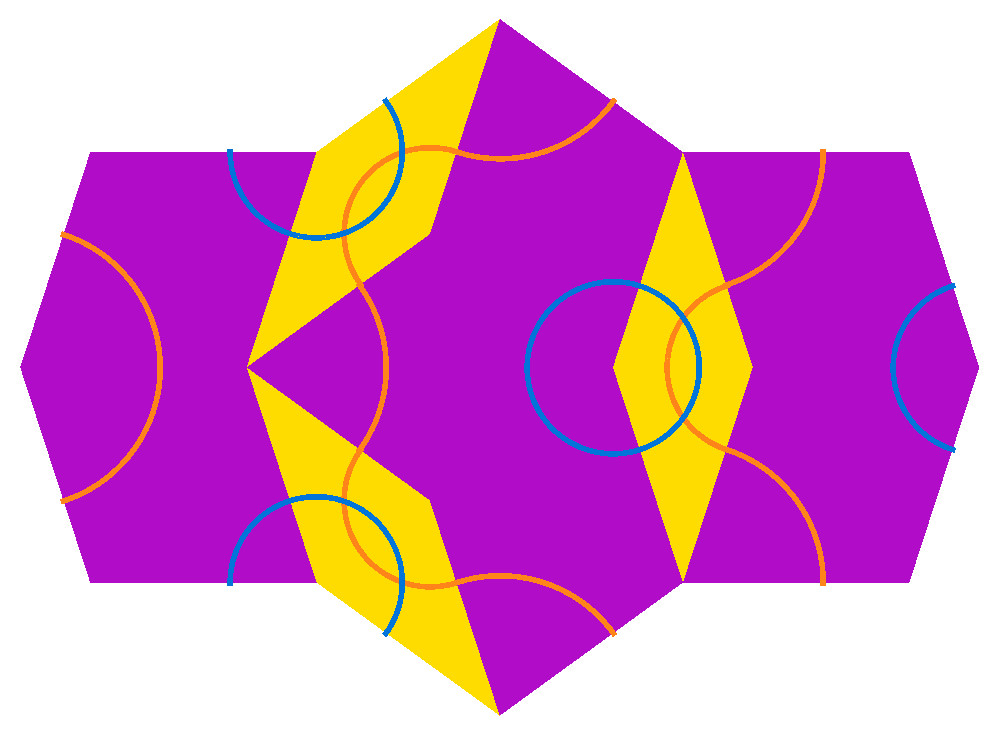
\includegraphics[scale=0.4]{FatInflation2}
             \end{subfigure}   &
             \begin{subfigure}[b]{0.4\textwidth}
             \centering
             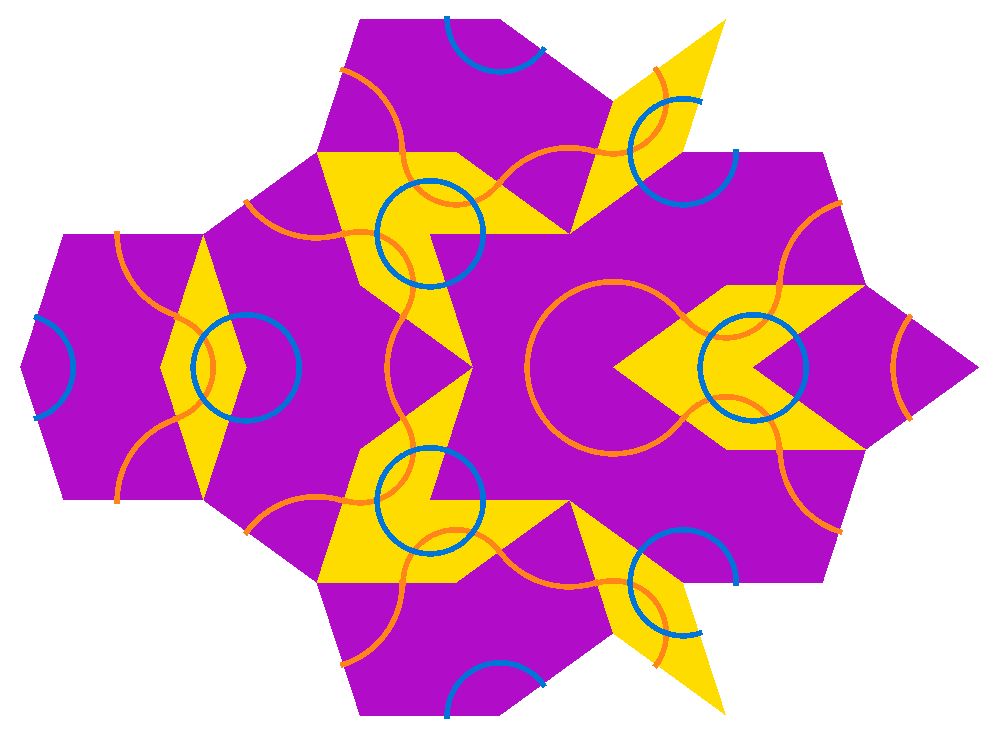
\includegraphics[scale=0.4]{FatInflation3}
             \end{subfigure}   \\
             \begin{subfigure}[b]{0.4\textwidth}
             \centering
             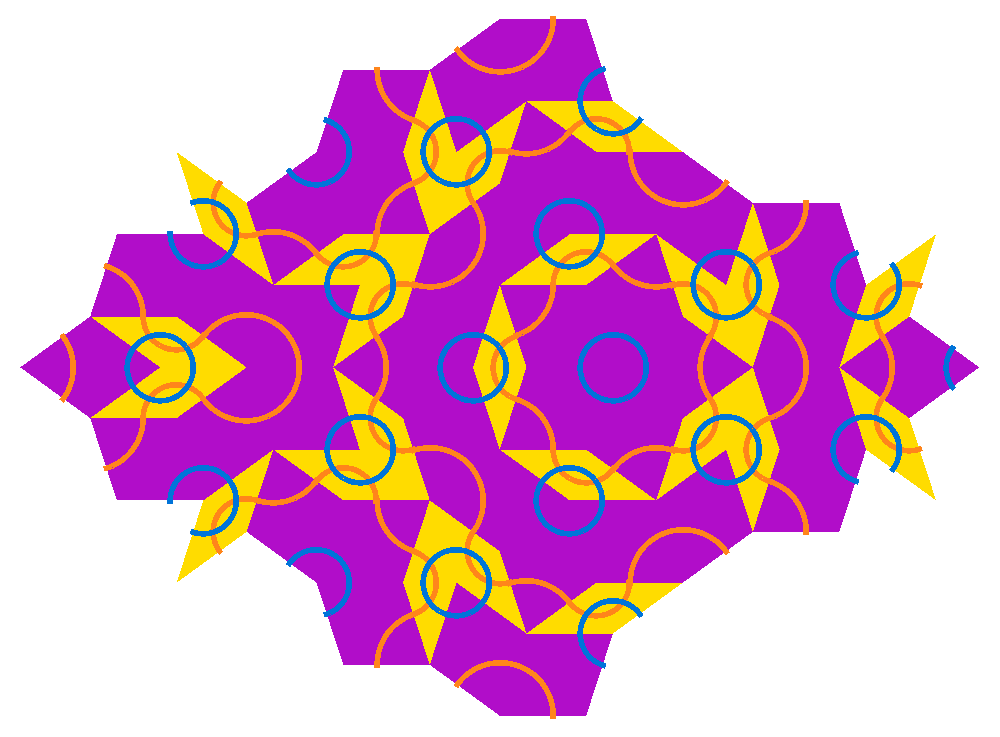
\includegraphics[scale=0.4]{FatInflation4}
             \end{subfigure}   &
             \begin{subfigure}[b]{0.4\textwidth}
             \centering
             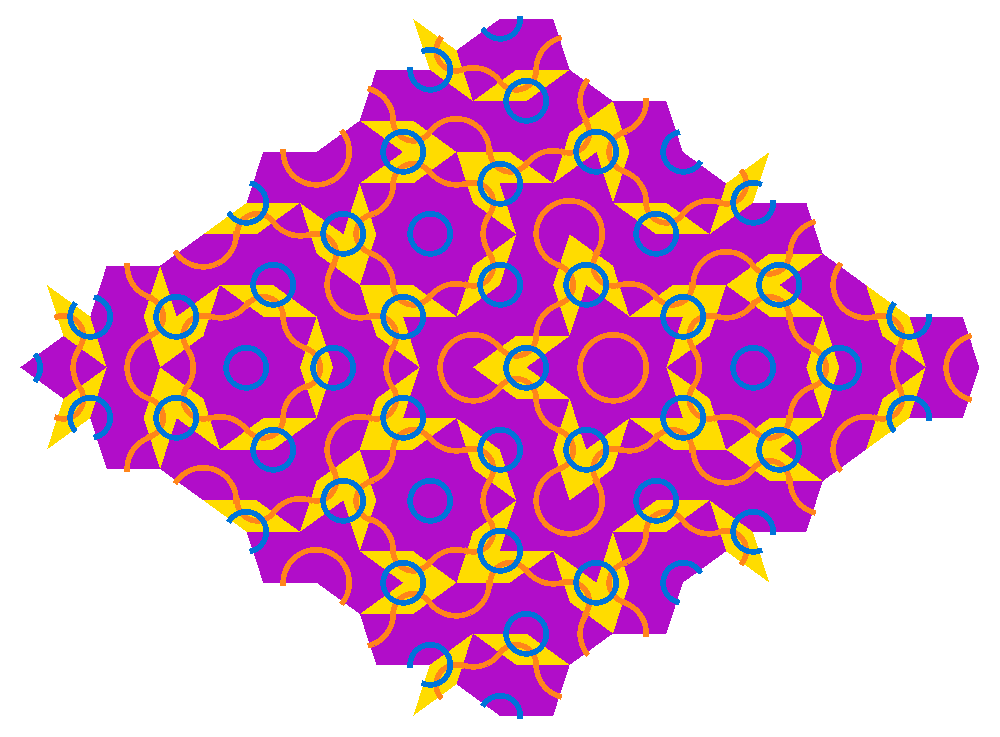
\includegraphics[scale=0.4]{FatInflation5}
             \end{subfigure}   \\
\end{tabular}
\caption[Successive of Deflations on Thick Rhomb]{Five successive iterations of the deflation process applied to the Thick Rhombus.}
\label{fig:ThickDeflate}
	\end{figure}

\begin{figure}[H]
\centering
\begin{tabular}{cc}
	        \begin{subfigure}[b]{0.4\textwidth}
	        \centering
	        \raisebox{0px}{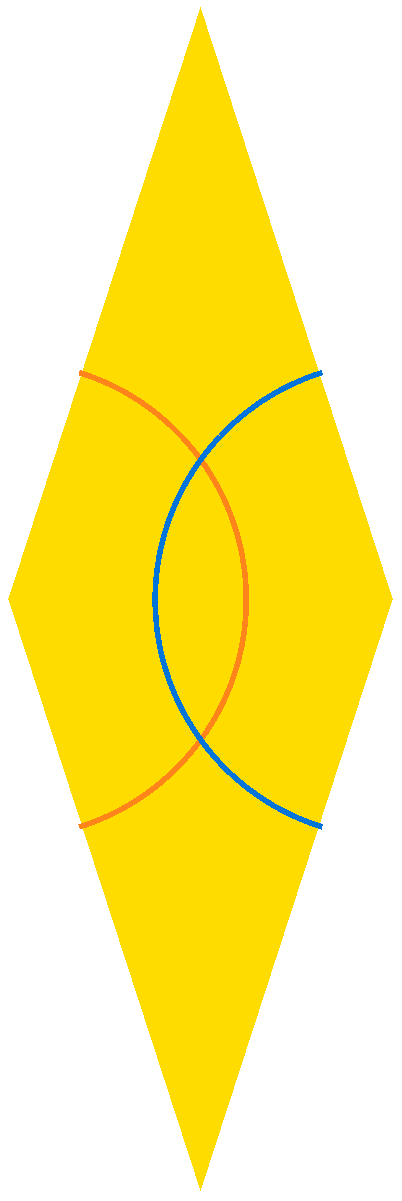
\includegraphics[scale=0.4]{SkinnyInflation0}}
	        \end{subfigure}   &
            \begin{subfigure}[b]{0.4\textwidth}
             \centering
             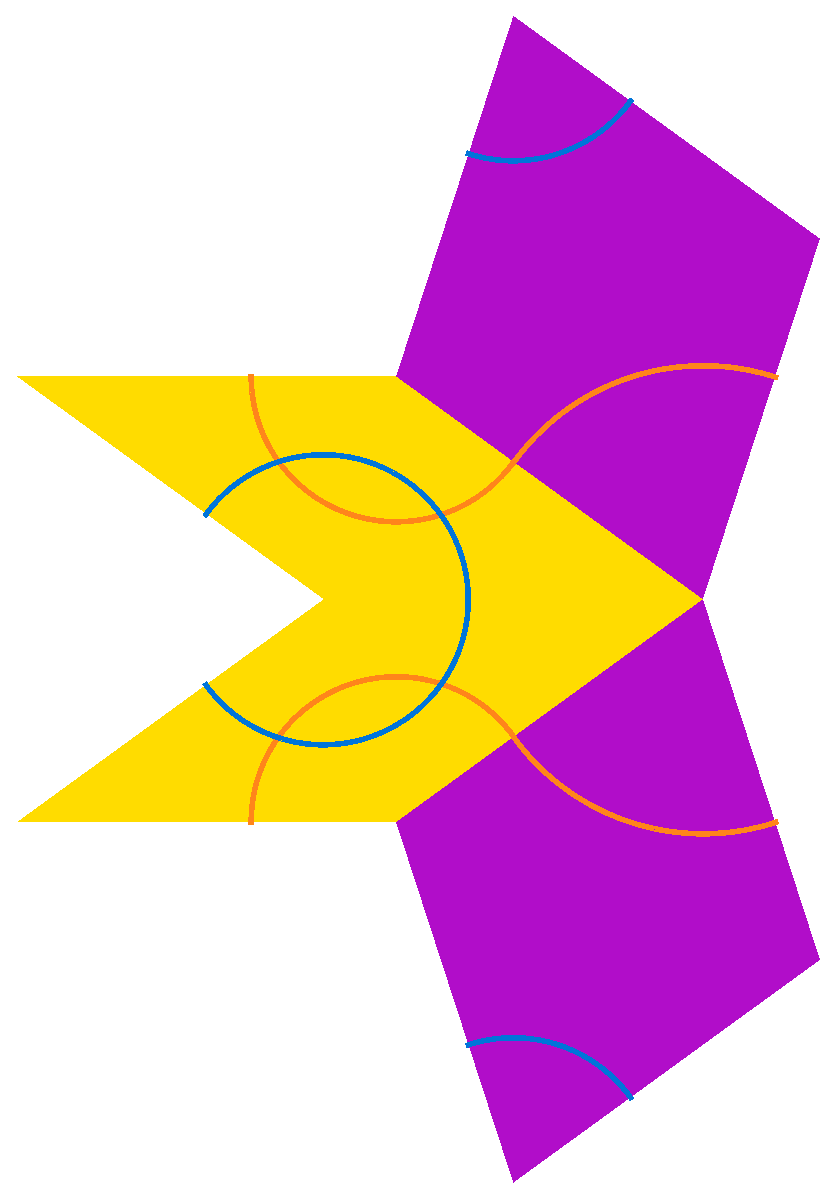
\includegraphics[scale=0.4]{SkinnyInflation1}
             \end{subfigure}   \\
	       	 \begin{subfigure}[b]{0.4\textwidth}
             \centering
             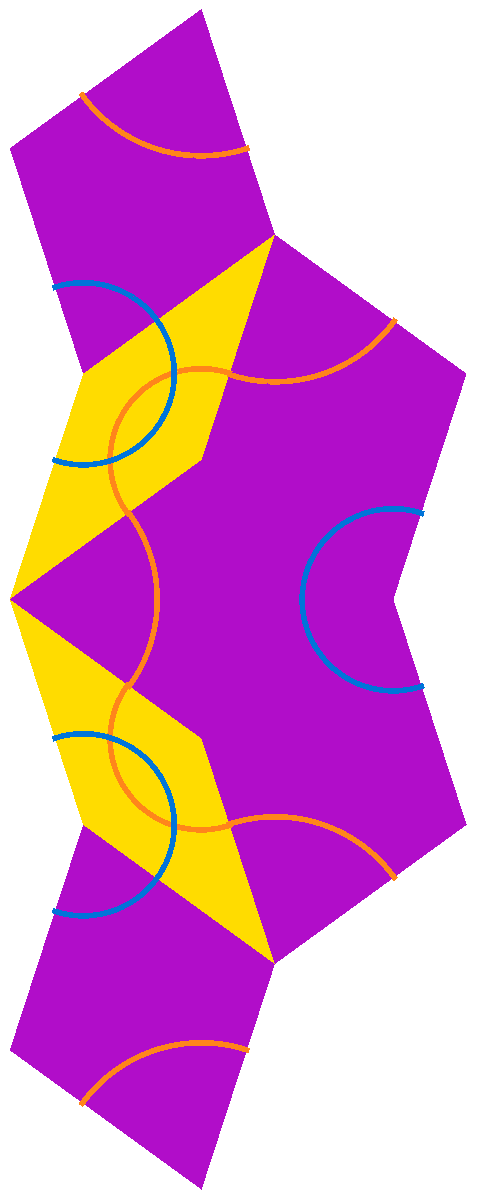
\includegraphics[scale=0.4]{SkinnyInflation2}
             \end{subfigure}   &
             \begin{subfigure}[b]{0.4\textwidth}
             \centering
             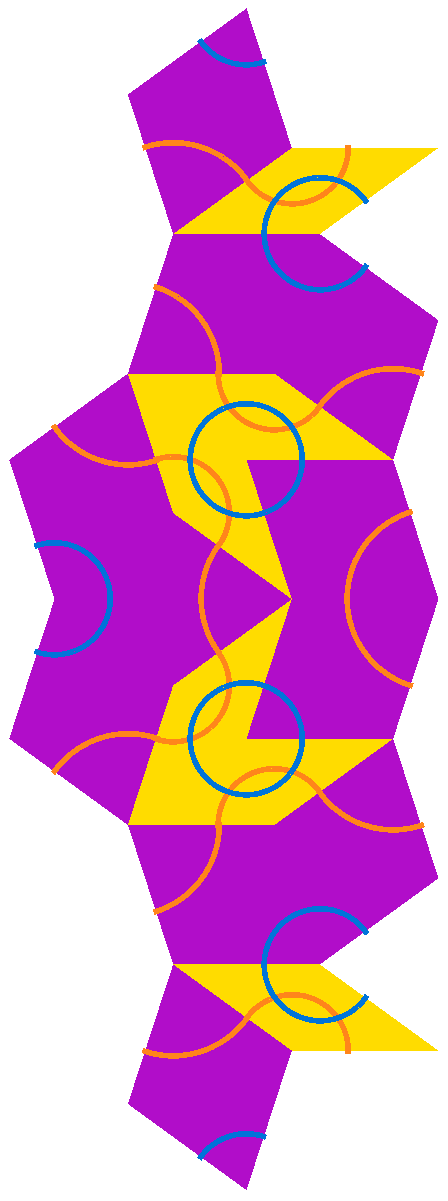
\includegraphics[scale=0.4]{SkinnyInflation3}
             \end{subfigure}   \\
             \begin{subfigure}[b]{0.4\textwidth}
             \centering
             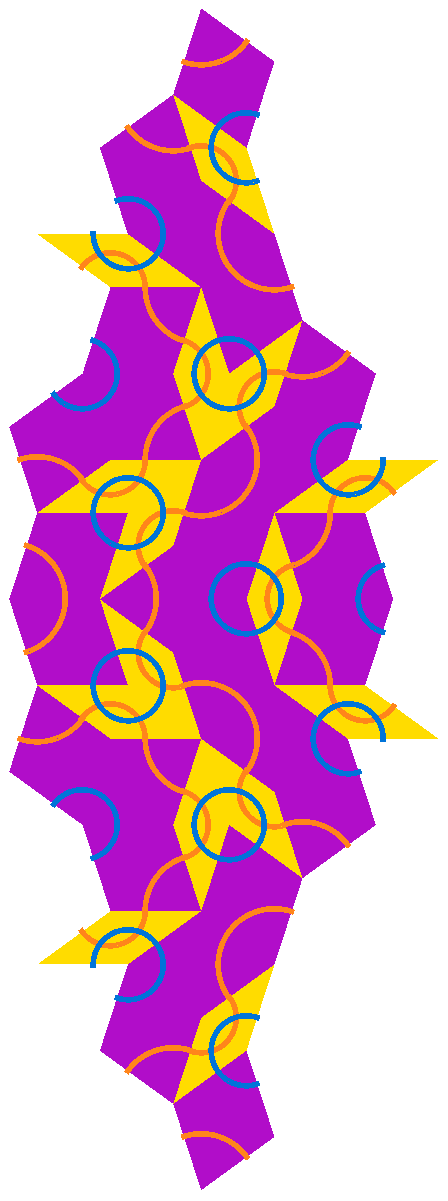
\includegraphics[scale=0.4]{SkinnyInflation4}
             \end{subfigure}   &
             \begin{subfigure}[b]{0.4\textwidth}
             \centering
             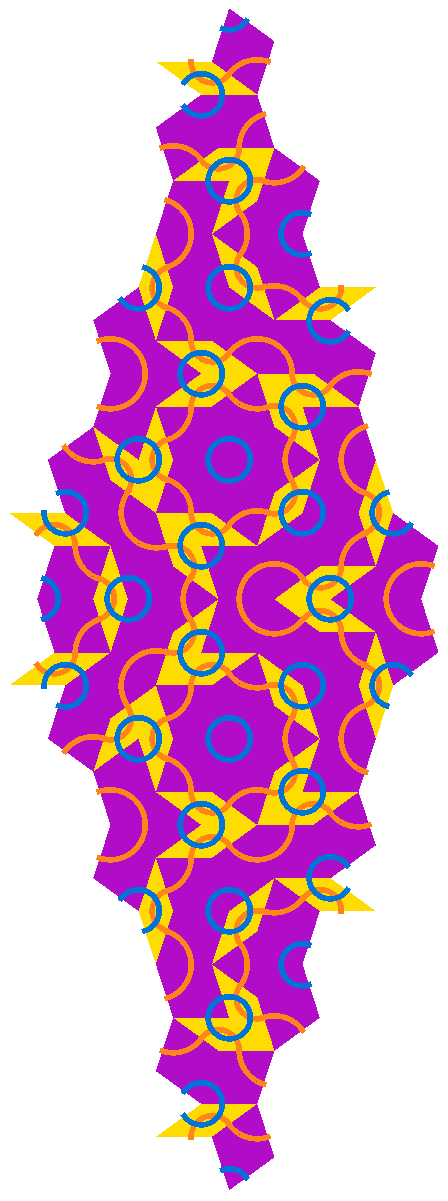
\includegraphics[scale=0.4]{SkinnyInflation5}
             \end{subfigure}   \\
\end{tabular}
\caption[Successive Deflations on Thin Rhomb]{Five successive iterations of the deflation process applied to the Thin Rhombus.}
\label{fig:ThinDeflate}
	\end{figure}
	

Notice that even after successive applications of the deflation substitution, the resulting tiling is still valid under the initial matching rules. Again, in Figures \ref{fig:ThickDeflate} and \ref{fig:ThinDeflate} this is illustrated by the continuity of the orange and blue edge-matching curves.

\section{Extension Theorem}
This substitution method is also called the deflation/inflation method, for the complementary processes described above. Where deflation applies successive substitutions to the Rhombs, and inflation scales the Rhombs back to their original size.

From Grunbaum and Shephard's \textit{Tilings and Patterns} we give the following important theorem for determining if a protoset will tile a plane \cite{Grunbaum1986}:
\begin{mythm}
\textbf{The Extension Theorem\\}
Let $\mathcal{P}$ be a finite set of prototiles. If $\mathcal{P}$ tiles over arbitrarily large circular disks, then $\mathcal{P}$ admits a tiling of the plane. \cite{Grunbaum1986,Ross}
\end{mythm}

\begin{mycor}
The Penrose Rhombs protoset admits tilings of the plane.
\end{mycor}

\begin{proof}
Under each iteration of the deflation, the substitution Rhombs are scaled by a factor of $\frac{1}{\phi}$. Consider the largest closed disk tiled completely by an arrangement of Rhombs. Under deflation each tile is scaled by  $\frac{1}{\phi}$, so the complementary inflation process will scale each tile by a factor of $\phi$. Therefore, the largest disk tiled completely by our substituted tiles will scale its diameter by at least a factor of $\phi$. For $n$ substitutions, the largest tiled disk will increase in diameter by at least $n\phi$. Therefore, deflation/inflation method can generate valid Penrose tilings of an arbitrary large disks in the plane.\\
$\therefore$ by Extension Theorem, the Penrose Rhombs admit tilings of the plane. 
\end{proof}





\chapter{Up-Down Construction} %DONE

In his 1990 paper \textit{Updown generation of Penrose patterns}, de Bruijn describes a construction method attributed to Conway by which tilings are generated by infinite sequences of steps along a directed graph \cite{DeBruijn1990}. The Up-Down generation process borrows some concepts from the substitution method, namely that we build tilings by \textbf{decomposing} tiles with constituent tiles, as per substitution rules. The key difference, however, is that we build a tiling instead by considering the relationship between a constituent tile and its inflation, that is, how constituent tiles \textbf{compose} parent tiles. As the name suggests, Up-Down generation constructs tilings through two processes: composition and decomposition or Up and Down.

In introducing this construction method, we must consider again the Robinson triangles. As with the substitution method, decomposition of these triangles is dependent on their orientation. Unlike substitution, the influence of triangle orientation under the Up-Down method is subtle and not automatic. Moving forward, we must be explicit with the triangle orientation, see Fig.\ref{fig:OrientedRob}. Further, recall from the substitution method that oriented Robinson triangles, arranged according to those matching rules, will determine a Penrose tiling of the plane by Penrose Rhombs. Robinson triangles can be transformed into Penrose Rhombs by reflection about their base, see Fig.\ref{fig:Rhombs}. As such, while the Up-Down method describes the process to construct a tiling of the plane by the oriented Robinson triangles of Fig.\ref{fig:OrientedRob}, we are also indirectly constructing a Penrose tiling by Rhombs. The relationship between these representations will be discussed in greater detail later, with the discussion of mutual local derivability. 

 

\begin{figure}[H]
        \begin{subfigure}[t]{0.4\textwidth}
                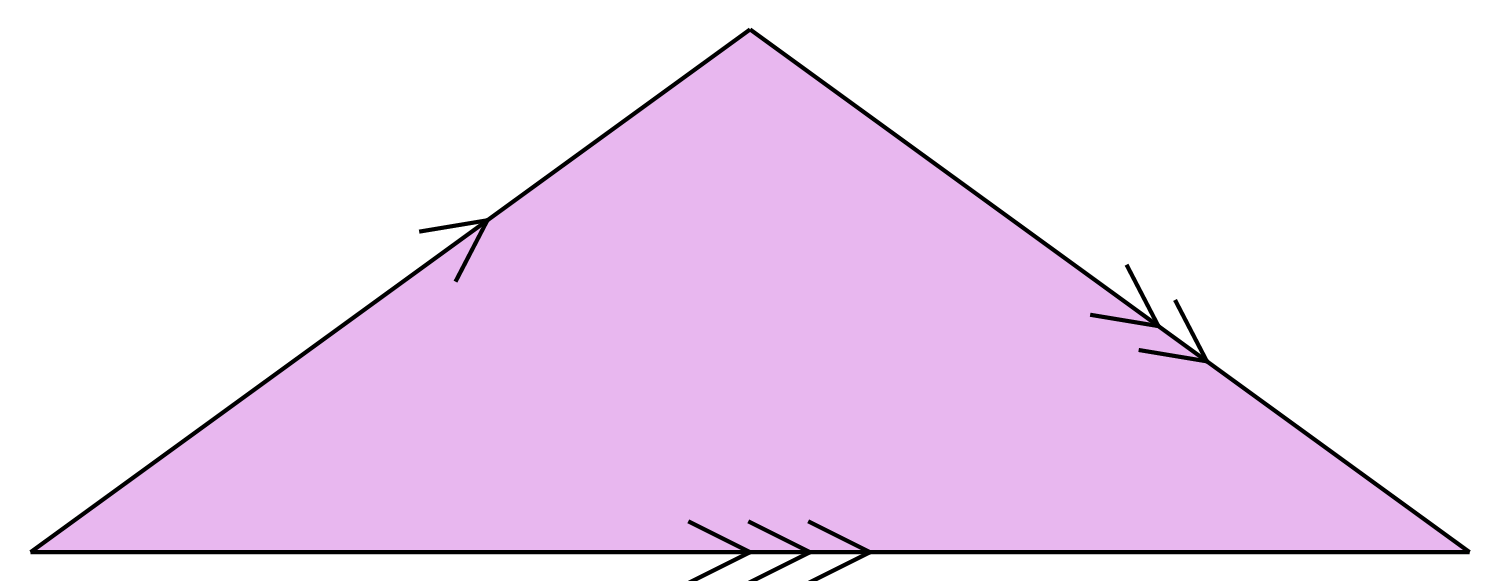
\includegraphics[width=\textwidth]{TFRob}
                \caption*{\Large T}
        \end{subfigure}\hfill
        \begin{subfigure}[t]{0.3\textwidth}
                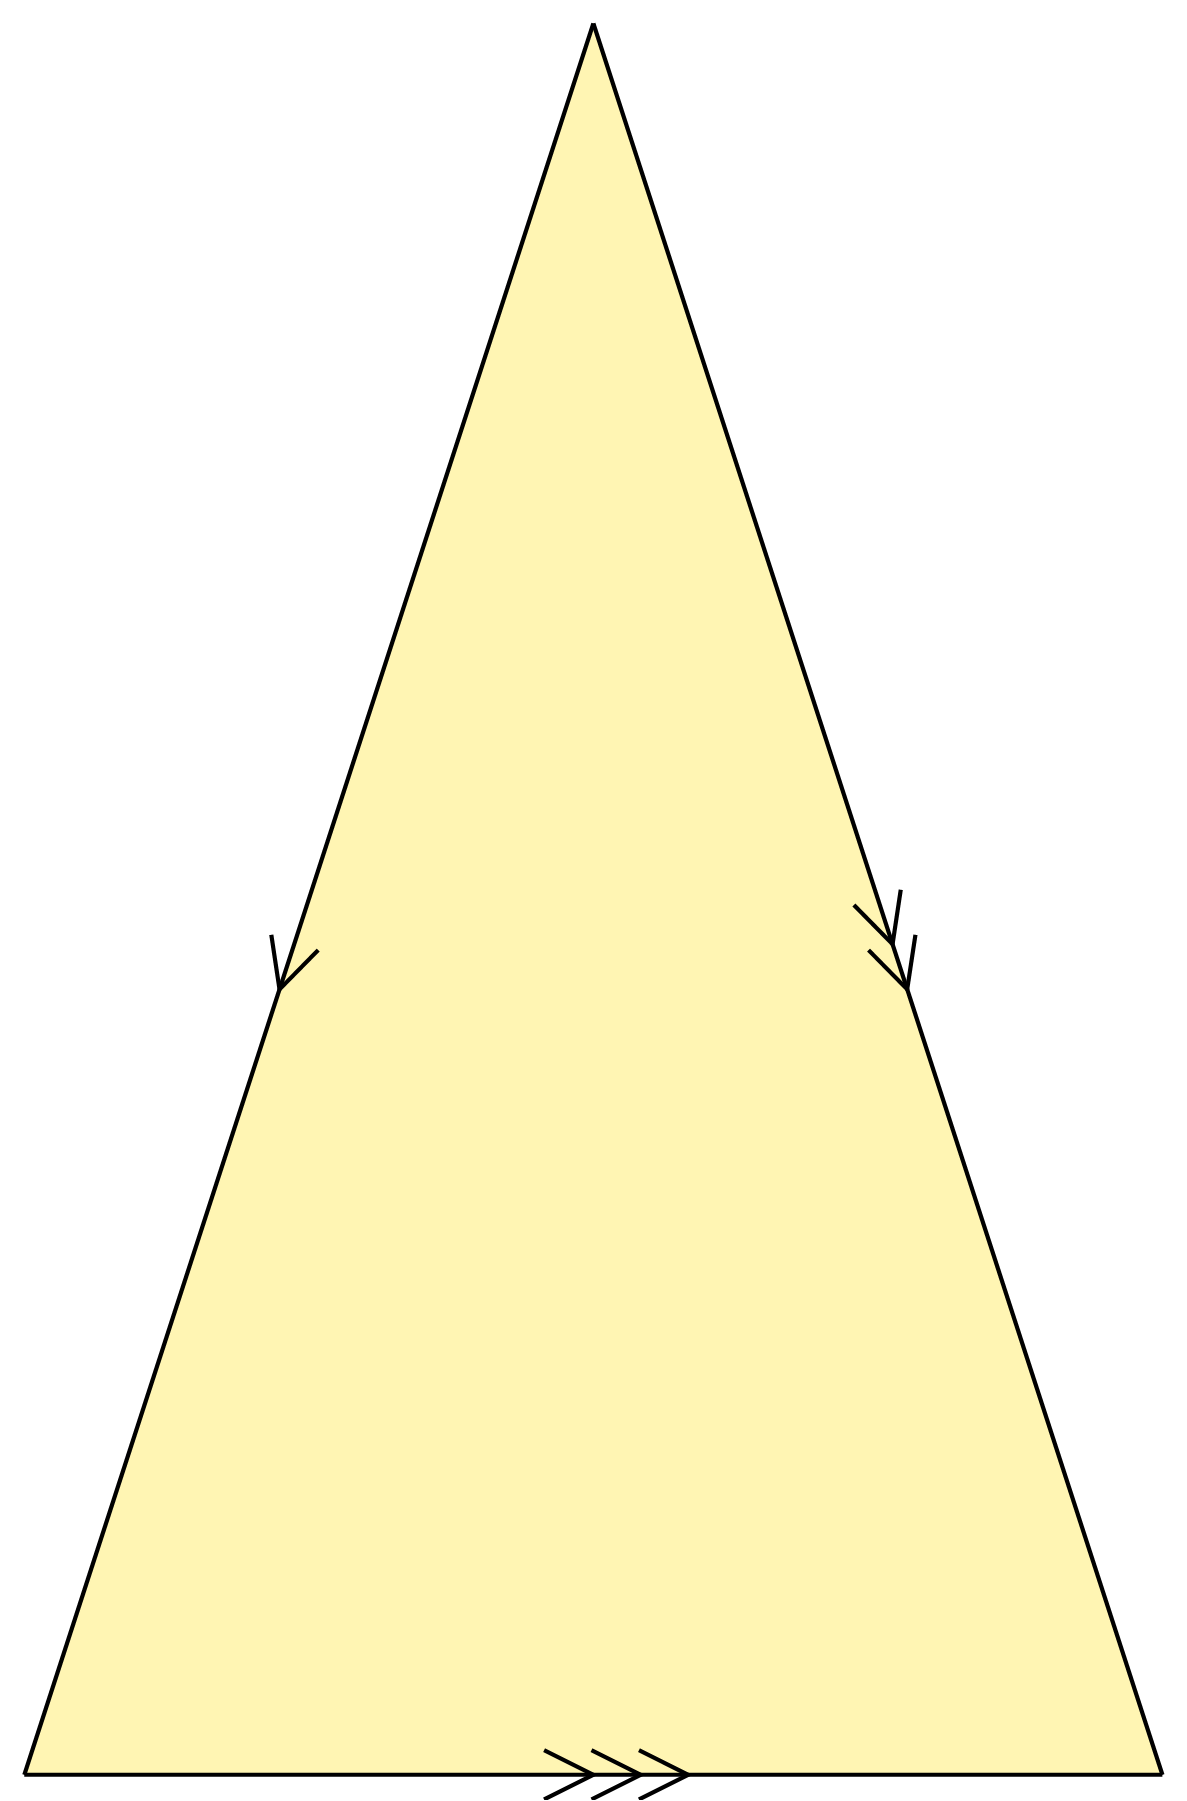
\includegraphics[width=\textwidth]{TSRob}
                \caption*{\Large t}
        \end{subfigure}\\
        
        \begin{subfigure}[t]{0.4\textwidth}
                \raisebox{0px}{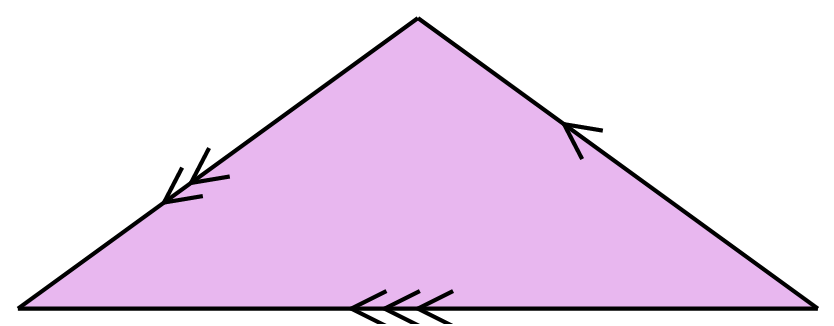
\includegraphics[width=\textwidth]{T'FRob}}
                \caption*{\Large T'}
        \end{subfigure}\hfill
        \begin{subfigure}[t]{0.3\textwidth}
                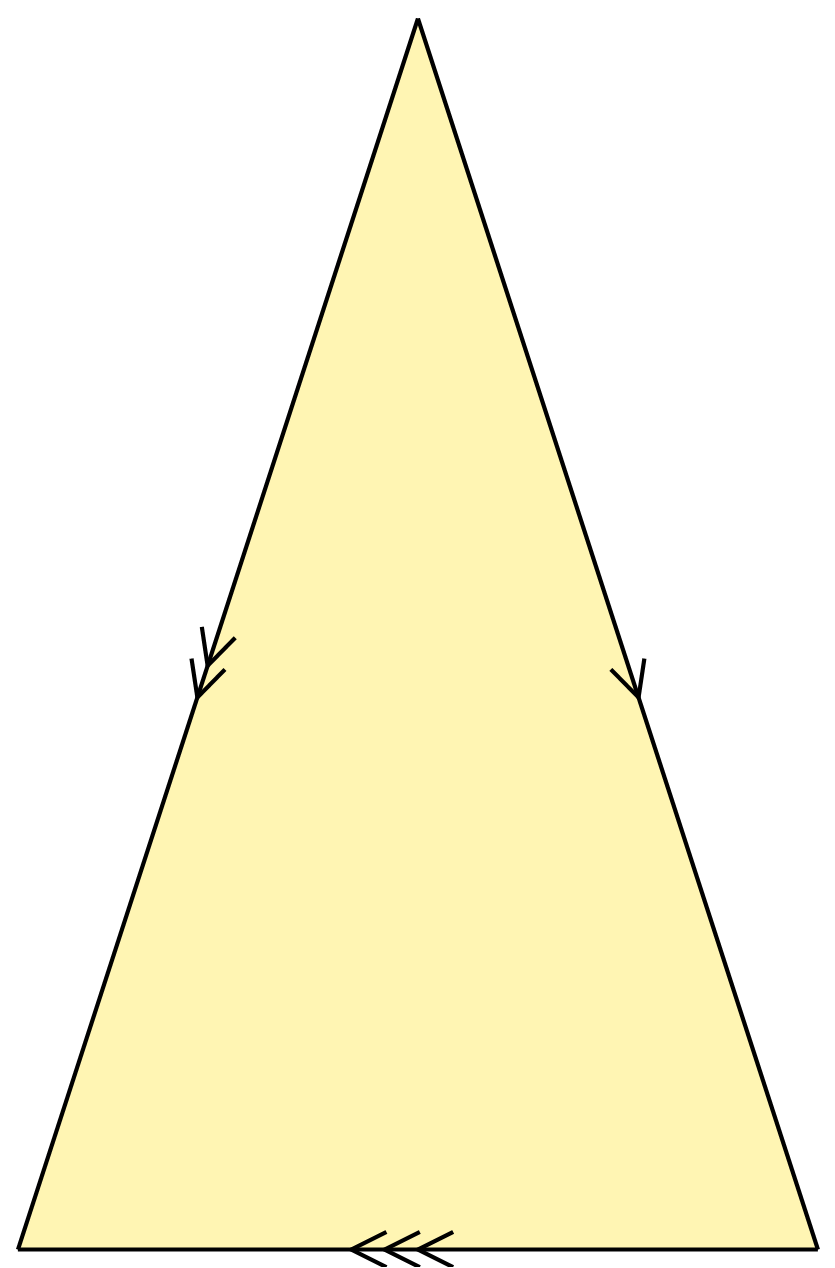
\includegraphics[width=\textwidth]{T'SRob}
                \caption*{\Large t'}
        \end{subfigure}  
        \caption[Oriented Robinson Triangles]{Oriented Robinson triangles. Thick or Obtuse Robinson Triangle is denoted with T. Thin or acute Robinson triangle is denoted with t. Reversed orientation is denoted with '. Arrowed edges illustrate Up-Down matching rules.}  
        \label{fig:OrientedRob}                    
\end{figure}

The matching rules under the substitution method behave slightly differently than the matching rules in the Up-Down method, illustrated with arrowed edges in Fig.\ref{fig:OrientedRob}. Here, the rules will indicate type and direction of edges, which must agree along abutting tiles. Additionally, the edge type and direction will satisfy decomposition rules according to the relationship between a triangle and it's constituent triangles, see Fig.\ref{fig:EdgeRules}. 

\begin{figure}[H]
        \begin{subfigure}[t]{0.4\textwidth}
                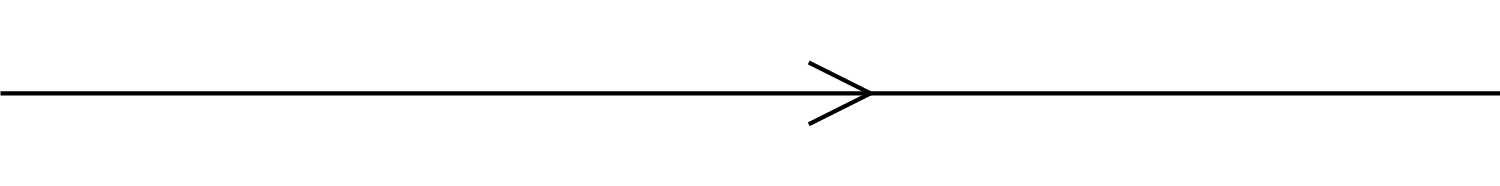
\includegraphics[width=\textwidth]{a1}
        \end{subfigure}\hfill
        \begin{subfigure}[t]{0.4\textwidth}
                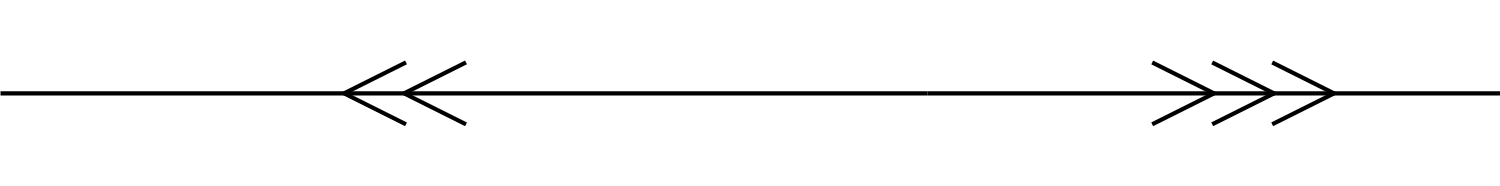
\includegraphics[width=\textwidth]{a1inflate}
        \end{subfigure}\\
        
        \begin{subfigure}[t]{0.4\textwidth}
                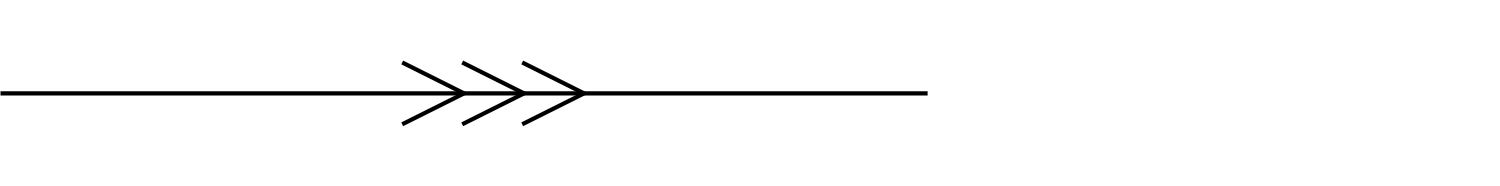
\includegraphics[width=\textwidth]{a2}
        \end{subfigure}\hfill
        \begin{subfigure}[t]{0.4\textwidth}
                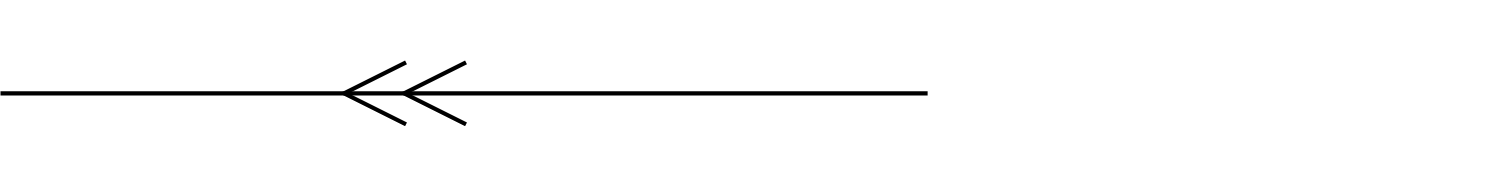
\includegraphics[width=\textwidth]{a2inflate}
        \end{subfigure}\\    
        
        \begin{subfigure}[t]{0.4\textwidth}
                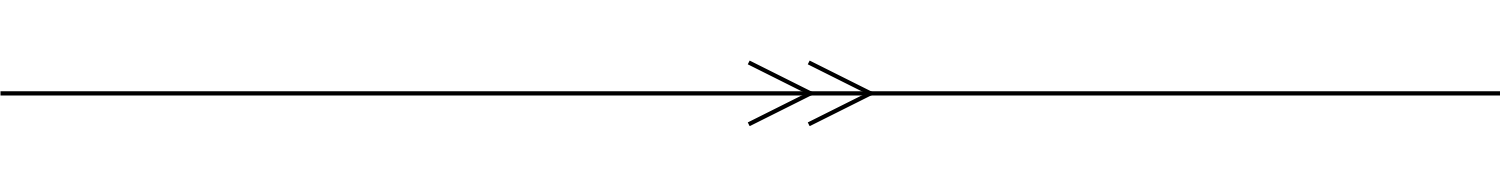
\includegraphics[width=\textwidth]{a3}
        \end{subfigure}\hfill
        \begin{subfigure}[t]{0.4\textwidth}
                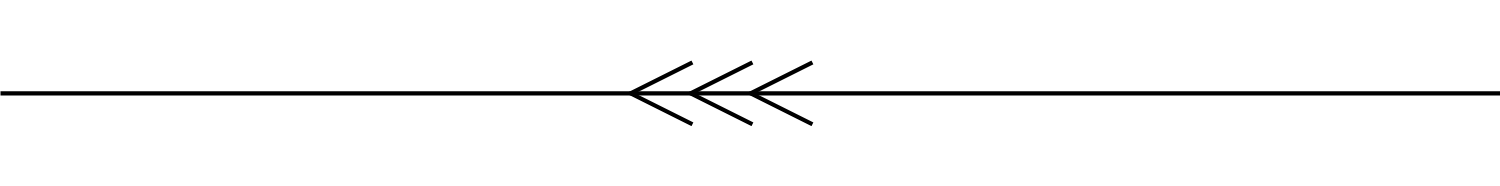
\includegraphics[width=\textwidth]{a3inflate}
        \end{subfigure}\\                           
        
        \begin{subfigure}[t]{0.4\textwidth}
                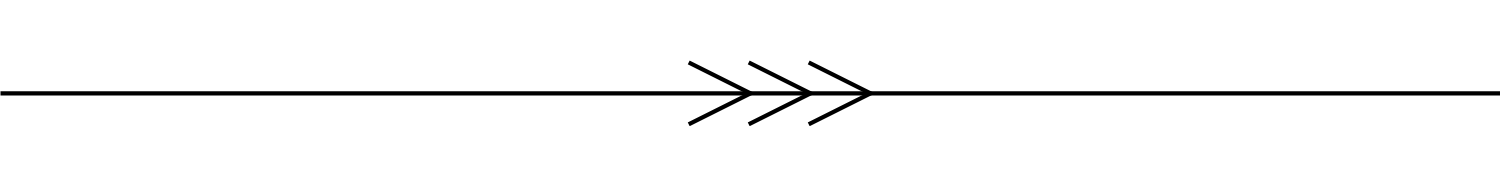
\includegraphics[width=\textwidth]{a4}
        \end{subfigure}\hfill
        \begin{subfigure}[t]{0.4\textwidth}
                \includegraphics[width=\textwidth]{a4inflate}
        \end{subfigure}\\   
        \caption[Edge Composition Rules]{Parent edges (Left) and their constituent edges (Right)}     
        \label{fig:EdgeRules}
\end{figure} 


\pagebreak
Consider again the substitution rules on the Robinson triangles described in Fig.\ref{fig:RobSubs}. This substitution is also employed in the Up-Down method. However, in this case we will label the constituent triangles of the substitution. We do this so we can explicitly describe how a constituent triangle composes a parent triangle. We label this composition relationship using mapping functions, given by lowercase Greek letters: $\alpha, \beta, \delta, \gamma$. We see the oriented Robinson triangles, substituted with relationship labels, in Fig.\ref{fig:OrientedSub}.

Composition relationships can be considered as mappings from a constituent triangle to its parent triangle. These composition mappings are as follows:
\begin{align}
\epsilon &: T \rightarrow T  &\epsilon' &: T' \rightarrow T' \nonumber\\  
\alpha &: T \rightarrow t  &\alpha' &: T' \rightarrow t' \nonumber\\  
\beta &: t \rightarrow t  &\beta' &: t' \rightarrow t' \label{eq:maps}\\  
\delta &: t' \rightarrow T  &\delta' &: t \rightarrow T' \nonumber\\ 
\gamma &: T' \rightarrow T  &\gamma' &: T \rightarrow T' \nonumber
\end{align}
Again, composition mappings are also labeled in Fig.\ref{fig:OrientedSub}. For an example of how to interpret a composition mapping, consider the mapping $\delta$ which maps constituent \textbf{t'} to parent \textbf{T}. This tells us that under composition by $\delta$, a yellow \textbf{t'} triangle will be compose a \textbf{T} parent.



\begin{figure}[H]
        \begin{subfigure}[t]{0.55\textwidth}
                \includegraphics[width=\textwidth]{TF}
        \end{subfigure}\hfill
        \begin{subfigure}[t]{0.35\textwidth}
                \includegraphics[width=\textwidth]{TS}
        \end{subfigure}\\
        
        \begin{subfigure}[t]{0.55\textwidth}
                \raisebox{55px}{\includegraphics[width=\textwidth]{TF'}}
        \end{subfigure}\hfill
        \begin{subfigure}[t]{0.35\textwidth}
                \includegraphics[width=\textwidth]{TS'}
        \end{subfigure}   
        \caption[Robinson Triangle Composition]{Oriented Robinson triangles with their constituent triangles. The relationship mappings between a constituent and parent triangles are given by lowercase Greek letters. For example, constituent triangle \textbf{T'} is related to parent triangle \textbf{T} under the mapping $\gamma$. The original edges of the parent triangles are also shown in grey. The relationship between the constituent and parent edges is shown in Fig.\ref{fig:EdgeRules}.}
        \label{fig:OrientedSub}                     
\end{figure}

From these mappings we can see why the explicit description of triangle orientation is necessary here. Otherwise, for instance, it would be ambiguous which constituent thick triangle, \textbf{T} or \textbf{T'}, we are describing inside a parent \textbf{T}.

We can alternatively visualize the mappings in Equations (\ref{eq:maps}) as directed graphs embedding constituent triangles into parent triangles, see Fig.\ref{fig:functionmap}. 

\begin{figure}[H]
        \begin{subfigure}[t]{0.6\textwidth}
                \includegraphics[width=\textwidth]{TRgraph}
        \end{subfigure}\hfill
        \begin{subfigure}[t]{0.4\textwidth}
                \includegraphics[width=\textwidth]{tsrgraph}
        \end{subfigure}\\
        
        \begin{subfigure}[t]{0.6\textwidth}
                \includegraphics[width=\textwidth]{TLgraph}
        \end{subfigure}\hfill
        \begin{subfigure}[t]{0.4\textwidth}
                \includegraphics[width=\textwidth]{tslgraph}
        \end{subfigure}  
        \caption[Composition Mappings]{Relationship mapping from constituent triangles to parent triangles given by Equations (\ref{eq:maps})} 
        \label{fig:functionmap}                    
\end{figure}

We are now ready to introduce the Up process. Realizing that composition mappings from Equations (\ref{eq:maps}) will place constituent triangles inside parent triangles, we see that each application of a mapping will generate a larger finite region of the tiling. Think of this process as the opposite of substitution, we are starting from a constituent and composing a  parent triangle. Just as substitution generated a finite section of a tiling, by mapping a constituent to a parent triangle we have similarly generated a finite section.

Further, just as with the substitution method, the end result of each mapping is an oriented Robinson triangle. That is, the image of every mapping will be the domain of other mappings. This allows us to form compositions of the mappings, from the image of one to the domain of another. To illustrate how these mappings can be composed from another, we have a cyclic directed graph in Fig.\ref{fig:UpDownGraph}.

\begin{figure}[H]
\centering
\includegraphics[width=\textwidth]{UpDownGraph}
\caption[Directed Graph of Composition Mappings]{A directed graph, or finite automaton, for the generation of parent triangles from constituent triangles. Paths along the directed edges represent compositions of the mappings from Equations (\ref{eq:maps}). Infinite paths along the directed edges may generate Penrose tilings of the plane.}
\label{fig:UpDownGraph}
\end{figure}

Paths along this directed graph represent compositions of the mappings. This is what is involved under the Up process, defining a sequence of the mappings. A finite sequence of mappings will directly correspond to a finite subregion of a Penrose tiling. Each sequential application of a mapping will describe a larger region of the tiling, and how the previous region composes into it. We can think of this process as hierarchically defining larger and larger regions by each sequential mapping.

The generation of the tiling region from the sequence of mappings is the Down process. Think of the Up process as producing a tiling instruction manual, and the Down process as following these instructions to produce a tiling. 

The Down process can describe a tiling region from the Up sequence because the mappings explicitly describe the relationship among decomposed triangles. Even though each mapping only directly describes the relationship between a constituent triangle and its parent, we have also uniquely determined the placement of the other constituent oriented Robinson triangles composing the parent. Further, the substitution rules from Fig.\ref{fig:OrientedRob} explicitly described the substitutions of the other constituent triangles. With this in mind, we can see how the Down process generates tiling regions from the Up process instructions. Essentially, the sequence of composition mappings from the Up process describes a sequence of decompositions, the Down process preforms these decompositions.

For an example of a finite sequence of the Up-Down process, consider the Up sequence from the graph path $\delta'\gamma\epsilon$ which defines the composition $\epsilon \circ \gamma \circ \delta'$. From the graph in Fig.\ref{fig:UpDownGraph} we can see that this Up sequence takes a \textbf{t} triangle and eventually embeds it into a \textbf{T} triangle. The Down process, given by this composition, then, will substitute that \textbf{T} triangle according to the composition sequence. This substitution ends once we've generated the initial \textbf{t} triangle. 


\begin{table}[H]
\begin{center}
\begin{tabular}{ccc}
\Large Up & & \Large Down\\
\raisebox{0px}{\includegraphics[width=0.3\textwidth]{Up4Left}} & \raisebox{20px}{\Large \textcolor{gray}{$ \rightarrow$}} & \includegraphics[width=0.6\textwidth]{Down4}\\
\Large $\uparrow$ $\epsilon$ & \hfill & $\downarrow$\\ 
\raisebox{0px}{\includegraphics[width=0.3\textwidth]{Up3Left}} & \raisebox{30px}{\Large \textcolor{gray}{$ \rightarrow$}} & \includegraphics[width=0.6\textwidth]{Down3}\\
\Large $\uparrow$ $\gamma$ & \hfill & $\downarrow$\\ 
\raisebox{0px}{\includegraphics[width=0.4\textwidth]{Up2Left}} & \raisebox{30px}{\Large \textcolor{gray}{$ \rightarrow$}} & \includegraphics[width=0.6\textwidth]{Down2}\\
\Large $\uparrow$ $\delta'$ & \hfill & $\downarrow$\\ 
\raisebox{0px}{\includegraphics[width=0.3\textwidth]{Up1Left}} &\raisebox{30px}{\Large \textcolor{gray}{$ \rightarrow$}}& \includegraphics[width=0.6\textwidth]{Down1}\\
\end{tabular}
\end{center}
\captionof{figure}[Up-Down Region Generation]{A finite region generated by the Up-Down process. The Up sequence $\delta'\gamma\epsilon$ describes the mapping composition $\epsilon \circ \gamma \circ \delta'$. The Up process maps a \textbf{t} triangle to a \textbf{T} triangle. The Down process applies those substitutions on a \textbf{T} triangle to generate the initial \textbf{t} triangle.}

\end{table}


Infinite sequences of the Up-Down process, corresponding to infinite paths along the directed graph, will generate Penrose tilings of the plane, half-plane, or $\frac{\pi}{5}$-plane wedge, depending on the sequence. Generating $\frac{\pi}{5}$-plane wedges are the result of repeated mappings into thin Robinson triangles, this occurs when the limit of the sequence generates a thin Robinson triangle. Effectively, wedges are when the `top' of the Up-Down process is an infinite \textbf{t} or \textbf{t'} triangle, and the Down process infinitely substitutes into this. Of course, under infinite sequences, the Up-Down process will have no `top' triangle, but we can see that certain arbitrarily long sequences can generate an arbitrarily large thin Robinson triangle tiling, and as such the limit of this process is the Penrose tiling of an infinite $\frac{\pi}{5}$-plane wedge. This is not a problem, however, in generating Penrose tilings of the entire plane, because these plane wedges can be extended to tilings of the plane by reflection along their edges. Reflections on the sides of wedges is valid under the edge matching rules, to illustrate this with finite thin Robinson triangles see Fig.\ref{fig:WedgeWheel}.  Penrose plane tilings generated by $\frac{\pi}{5}$-plane wedge reflection will exhibit fivefold rotational symmetry centered at the point of the wedge. As we will discuss later, five-fold rotational symmetry is only possible in aperiodic tilings, so this is a remarkable feature of Penrose tilings generated from plane wedges. Similarly, half-plane tilings occur when the limit of the process is an arbitrarily large thick Robinson triangle. Half-plane tilings can also be extended to full plane tilings by reflection across the base.

\begin{figure}
\centering
\includegraphics[width=0.5\textwidth]{WedgeWheel}
\caption[Reflection along $\frac{\pi}{5}$-plane Wedge Edges]{Reflection along sides of thin Robinson triangles produces valid arrangement of triangles under the edge matching rules. Demonstrated for finite triangles, this is also true for infinite  $\frac{\pi}{5}$-plane wedges. As such,  $\frac{\pi}{5}$-plane wedges can be extended to tilings of the entire plane under side reflection. Planes tiled in this way will exhibit fivefold rotational symmetry about the wedge point.}
\label{fig:WedgeWheel}
\end{figure}

\section{Penrose Tilings as Infinite Sequences}
We've seen how the Up-Down method generates Penrose tilings from infinite compositions of mappings. By describing these infinite compositions as sequences, we've alluded to an alternative representation of a Penrose tiling, as an infinite sequence of steps on the directed graph in Fig.\ref{fig:UpDownGraph}. 

\begin{mydef}
A \textbf{composition sequence}, $\rho$, is an infinite sequence of mappings which, under the Up-Down process, will take an elementary Robinson triangle to a Penrose tiling of the plane, half-plane, or $\frac{\pi}{5}$-plane wedge. Compositions sequences must correspond to infinite paths on the graph in Fig.\ref{fig:UpDownGraph}.
\end{mydef}

\begin{mylem}
Every composition sequence generates a Penrose tiling of a plane, half-plane, or $\frac{\pi}{5}$-plane wedge.
\end{mylem}

\begin{proof}
This follows directly from the Up-Down method.
\end{proof}

By the above lemma, we see that every composition sequence generates a Penrose tiling. However, Penrose tilings are not unique to a composition sequence.

\begin{mylem}
A Penrose tiling is generated by infinitely many composition sequences.
\end{mylem}

\begin{proof}
Consider a Penrose tiling, $\mathcal{T}$.\\
$\mathcal{T}$ is composed of infinitely many individual tiles.\\
By the Up-Down method, each tile can generate $\mathcal{T}$ by a unique composition sequence.\\
$\therefore$ There are infinitely many composition sequences which generate $\mathcal{T}$.
\end{proof}

We've now shown that while all composition sequences correspond to a Penrose tiling, this relationship isn't one-to-one. That is, we see that infinitely many sequences generate the same Penrose tiling. What determines whether the same Penrose tiling is generated by two different sequences?

\begin{mydef}
Two composition sequences, $\rho_1$ and $\rho_2$, are said to be \textbf{cofinal} if they agree after finitely many terms.
\end{mydef}

\begin{mythm}
Two composition sequences generate the same Penrose tiling if and only if they are cofinal.
\end{mythm}

\begin{proof}
Let $\rho_1$ and $\rho_2$ be composition sequences defining $\mathcal{T}_1$ and $\mathcal{T}_2$ respectively. \\[10pt]
If $\rho_1 = \rho_2$ then $\mathcal{T}_1 = \mathcal{T}_2$, and they are trivially cofinal.\\[10pt]
If $\rho_1$ and $\rho_2$ are cofinal, then, after, $n$, finitely many terms, the sequences agree.\\
Consider composition sequence, $\rho^*$, which begins where $\rho_1$ and $\rho_2$ agree.\\
$\rho^*$ defines a Penrose tiling  $\mathcal{T}^*$.\\
This implies that, at some hierarchal level, level $n$ in the Up process, $\rho_1$ and $\rho_2$ begin describing the same tiling.\\
By the Up-Down process, substitution is uniquely defined.\\
Therefore, $\mathcal{T}^*$ uniquely determines $\mathcal{T}_1$ after $n$ substitutions.\\
Likewise, $\mathcal{T}^*$ uniquely determines $\mathcal{T}_2$ after $n$ substitutions.\\
$\therefore$ $\mathcal{T}_1 = \mathcal{T}_2$ if  $\rho_1$ and $\rho_2$ are cofinal.\\[10pt]
Conversely, suppose $\mathcal{T}_1 = \mathcal{T}_2$ and call this tiling $\mathcal{T}$. \\
Let $\rho_1$ begin with the tile  ${\rho_1}_0$.\\
Let $\rho_2$ begin with the tile ${\rho_2}_0$.\\
Then ${\rho_1}_0$ and ${\rho_2}_0$ both belong to $\mathcal{T}$.\\
The distance between ${\rho_1}_0$ and ${\rho_2}_0$ is therefore finite.\\
Then at some hierarchal level, after finite $n$ in the Up process, a single tile will contain both ${\rho_1}_0$ and ${\rho_2}_0$.\\
$\rho_1$ and $\rho_2$ will agree after this level.\\
$\therefore$ $\rho_1$ and $\rho_2$ are cofinal if $\mathcal{T}_1$ and $\mathcal{T}_2$.
\end{proof}

We now see that all cofinal sequences are related to each other by the unique Penrose tiling they generate. This defines an equivalence class.

\begin{mydef}
Cofinality of composition sequences defines an equivalence relation on the set of composition sequences. Equivalence classes of cofinal sequences are called \textbf{families}.
\end{mydef}

Further, we can consider a function, $C(\rho)$, which takes a composition sequence and returns its parent sequence. In other words, if $\rho$ defines a Penrose tiling, $C(\rho)$ defines the tiling before the previous substitution. 

\begin{mylem}
$\rho$ and $\rho'$ are cofinal if and only if $C(\rho)$ and $C(\rho')$ are cofinal.
\end{mylem}

\begin{proof}
Let 
\begin{equation*}\begin{split}
\rho=\{\rho_0,\rho_1,\rho_2,\rho_3,\mathellipsis\}\\
\rho'=\{\rho'_0,\rho'_1,\rho'_2,\rho'_3,\mathellipsis\}
\end{split}
\end{equation*}\\
Then 
\begin{equation*}
\begin{split}
C(\rho)=\{\rho_1,\rho_2,\rho_3,\mathellipsis\}\\
C(\rho')=\{\rho'_1,\rho'_2,\rho'_3,\mathellipsis\}
\end{split}
\end{equation*}\\
By definition of cofinality and inspection, $\rho$ and $\rho'$ are cofinal if and only if $C(\rho)$ and $C(\rho')$ are cofinal.
\end{proof}

Further, $C(\rho)$ allows us to address a common misconception regarding Penrose tilings. When looking at a graphical representation of a tiling, especially when considering their construction by substitution, it is easy to assume that the Penrose tiling is self-similar. We can easily show this is not the case in general.

\begin{mylem}
Penrose tilings are, in general, not self-similar.
\end{mylem}

\begin{proof}
Consider a Penrose tiling, $\mathcal{T}$.\\
$\mathcal{T}$ is given by composition sequence $\rho$.\\
In general, $C(\rho)\neq\rho$.\\
$\therefore$ Penrose tilings are not self-similar.
\end{proof}

However, we arrive at something of a veridical paradox here. We've just shown that Penrose tilings are not self-similar. However, we also know that, trivially, $\rho$ and $C(\rho)$ are cofinite. Therefore, we see that $\rho$ and $C(\rho)$ define the same Penrose tiling. That is, substitution of a Penrose tiling will map the tiling back to itself, but this will not be self-similar. 

Finally, we are ready to see the greatest benefit to considering Penrose tilings as equivalence classes of composition sequences.

\begin{mythm}
There are uncountably many Penrose tilings.
\end{mythm}

\begin{proof}
Every Penrose tiling is uniquely determined by a family of cofinal composition sequences.\\
By Cantor's Diagonalization Argument, if there were countably many Penrose tilings then we could construct a countable list of infinite sequences, with one sequence from each family.\\
However, by considering infinite paths on the directed graph or recalling the proof of the uncountability of real numbers, we see that given such a countable list we can always construct a composition sequence that is not a member of that list.\\
Therefore, a countable list of composition sequence families will always be incomplete.\\
Therefore, there are uncountably many composition sequence families.\\
$\therefore$ there are uncountably many Penrose tilings by Cantor's Diagonalization.
\end{proof}
\chapter{Pentagrid Construction}
\section{Duals}
As we will see, one useful way to determine a tiling is to describe its \textbf{dual}. \cite{Effinger2006}

\begin{mydef}
Two tilings, $\mathcal{T}$ and $\mathcal{T}'$, are \textbf{dual} if 
\begin{enumerate}
\item There exists one-to-one mappings from the vertices, edges, and faces of $\mathcal{T}$  to the faces, edges, and vertices of $\mathcal{T}'$, respectively.
\item If a face, $\mathcal{F}$ in $\mathcal{T}$ contains a vertex, $v$ in $\mathcal{T}'$ then the faces in $\mathcal{T}'$ belonging to $v$ will contain vertices belonging to $\mathcal{F}$. 
\end{enumerate}
\end{mydef}

\begin{mydef}
Two dual tilings, $\mathcal{T}$ and $\mathcal{T}'$, are \textbf{orthogonally dual} if each edge in $\mathcal{T}$ is orthogonal to its corresponding edge in $\mathcal{T}'$.
\end{mydef}

For example, consider the hexagonal tiling and its orthogonal dual tiling in Fig.\ref{fig:Hexagons}. Each face of the hexagonal tiling is in one-to-one correspondence with a vertex of the equilateral triangle tiling. Each vertex of the hexagonal tiling is in one-to-one correspondence with a face of the equilateral triangle tiling. The edges of the tilings are also in one-to-one correspondence and orthogonal. 

\begin{figure}[H]
\centering
\includegraphics[width=0.7\textwidth]{HexagonDuals}
\caption[Hexagonal Tiling Dual]{A hexagonal tiling, $\mathcal{T}$, has a dual tiling, $\mathcal{T}'$, of equilateral triangles (purple). As defined, there is a one-to-one correspondence between the hexagonal faces of $\mathcal{T}$ and the vertices (blue) of $\mathcal{T}'$. Likewise, there is a one-to-one correspondence between the triangular faces of $\mathcal{T}'$ and the vertices (red) of $\mathcal{T}$. Further, these tilings are orthogonal duals, so each edge of $\mathcal{T}$ (black) is in one-to-one correspondence and orthogonal to an edge of $\mathcal{T}'$ (purple).}
\label{fig:Hexagons}
\end{figure}

Consider that the equilateral triangle tiling is given by three families of equally spaced lines, superimposed and rotated by $\frac{\pi}{3}$, which we will call the trigrid (see Fig.\ref{fig:trifam}). As we've seen in Fig.\ref{fig:Hexagons}, the equilateral triangle tiling is the orthogonal dual of the hexagonal tiling. We, then, can consider the hexagonal tiling to be completely determined by the points of intersection of the trigrid. 

\begin{figure}[H]
\centering
\includegraphics[width=0.4\textwidth]{TriangleFamilies}
\caption[Trigrid]{Three families of parallel, equally spaced lines, the trigrid, coloured orange, purple, and blue. The families, superimposed and rotated by $\frac{\pi}{3}$ from each other, give the equilateral triangle tiling.}
\label{fig:trifam}
\end{figure}

It is important to note that this is an idealized example for the visualization of tiling duals. We are able to superimpose the hexagonal tiling and the equilateral triangle tiling in a meaningful way. However, from our definition of dual, this is not a requirement. To understand how tilings can be duals, without being superimposable, consider Fig.\ref{fig:hexsmall}. Here we see a hexagonal tile placed at each intersection point of the trigrid. The six rays of the trigrid from each intersection point meet the edges of the hexagon orthogonally. Further, the intersections of the trigrid uniquely determine the configuration of the hexagonal tiles. Observe in Fig.\ref{fig:hexsmall} that each triangle face contains three hexagonal vertices. Since these are dual tilings, those three hexagonal vertices must correspond to the same vertex in a hexagonal tiling. Likewise, notice that each equilateral triangle edge meets two hexagonal tile edges, therefore those two hexagons must abut in a hexagonal tiling.  We see that the trigrid completely determines the hexagonal tiling. 

\begin{figure}[H]
\centering
\includegraphics[width=0.6\textwidth]{HexagonDualSmall}
\caption[Hexagons Defined by Trigrid Intersections]{A hexagonal tiling is completely determined by the intersections of the trigrid in Fig.\ref{fig:trifam}. We can see how each intersection uniquely describes a hexagonal tile, with the lines orthogonally meeting the edges of the tile. Notice that each triangle face contains three hexagonal vertices, example highlighted in red. By the definition of dual, these vertices must meet at a single vertex in the hexagonal tiling. Likewise, each triangle edge meets with two hexagon edges, an example of this is shown in red. Therefore, these edges must correspond to a single edge of the hexagonal tiling. Thus, the trigrid uniquely determine the configuration of the hexagon tiles.}
\label{fig:hexsmall}
\end{figure}

It is useful to construct tilings by their duals in this way if, as above, the duals can be given as intersecting families of lines. Constructing tilings in this way equips us with tools from other fields of mathematics, especially projective and algebraic methods.

\section{Regular Pentagrids}
Here we will describe a pentagrid, constructed similarly to the trigrid, but with five families of parallel lines. Consider, first, the fifth roots of unity, vectors pointing to the vertices of a regular pentagon (see Fig.\ref{fig:rootsunity}):
\begin{equation*}
\vec{\epsilon}_i= e^{\frac{2 \pi \mathrm{i}}{5}} \qquad \qquad i=\{0,1,2,3,4\}\\
\end{equation*}
\begin{figure}[H]
\centering
\includegraphics[width=0.3\textwidth]{RootsUnity}
\caption[Fifth Roots of Unity]{The fifth roots of unity. Vectors point to the vertices of a regular pentagon.}
\label{fig:rootsunity}
\end{figure}

We will refer to these vectors as \textit{grid vectors}. Now, as with the trigrid, consider five families of equally spaced parallel lines, superimposed and rotated $\frac{2\pi}{5}$. As seen in Fig.\ref{fig:singularpentagrid}, each family corresponds to a grid vector, meeting that grid vector orthogonally. Further, the distance between consecutive lines in a family is $\frac{1}{|\vec{\epsilon}|}$.
\begin{figure}[H]
\centering
\includegraphics[width=0.5\textwidth]{SingularPentagrid}
\caption[Singular Pentagrid]{Five families of equally spaced parallel lines, superimposed and rotated about the origin by $\frac{2\pi}{5}$. Each family corresponds to one grid vector, meeting it orthogonally. For example, the orange family corresponds to the $\vec{\epsilon}_0$ grid vector. This forms a singular pentagrid, as all families of lines meet at the origin.}
\label{fig:singularpentagrid}
\end{figure}

The families of the above grid all intersect at the origin. We consider this grid a \textit{singular pentagrid}. We describe this pentagrid as \textit{singular} because more than two lines intersect at any point. However, as we will see, we are interested only in pentagrids with the property that no more than two grid lines intersect at any point, we call such pentagrids \textit{regular}.

To construct regular pentagrids, we shift a family of grid lines from the origin by a \textit{shift factor}, $\gamma_i \in \mathbb{R}$, in the direction of its corresponding grid vector $\vec{\epsilon}_i$, see Fig.\ref{fig:regularpentagrid}. All points on the grid in such a shifted pentagrid will satisfy the \textit{grid equation}:
\begin{equation}
\vec{x}\cdot\vec{\epsilon}+\gamma=k \quad k\in\mathbb{Z}
\end{equation}

If a line on grid $i$ satisfies the equation
\begin{equation}
\vec{x}\cdot\vec{\epsilon}_i+\gamma=k_i \quad k_i\in\mathbb{Z}
\end{equation}
then the line has \textit{index} $k_i$.

\begin{figure}[H]
\centering
\includegraphics[width=0.5\textwidth]{RegularPentagrid}
\caption[Regular Pentagrid]{We shift each family of grid lines by a shift factor,  $\gamma_i$, in the direction if its corresponding grid vector, $\vec{\epsilon}_i$. A shifted pentagrid will be regular if it satisfies de Bruijn's sum condition in Eq.\ref{eq:sumcondition}.}
\label{fig:regularpentagrid}
\end{figure}

De Bruijn proved that a pentagrid will be regular if its shift factors satisfy a sum condition:
\begin{equation}
\sum_{i=0}^{4}\gamma_i=0
\label{eq:sumcondition}
\end{equation}

Recall from our definition of regular that each intersection of such a pentagrid will occur only between two lines. Further, we can see that these intersections only occur at angles of $\frac{\pi}{5}$ or $\frac{2\pi}{5}$, see Fig.\ref{fig:intersections}.

\begin{figure}[H]
\centering
\begin{subfigure}[b]{0.5\textwidth}
\centering
\includegraphics[width=0.6\textwidth]{Intersection1}
\caption{$\frac{\pi}{5}$}
\end{subfigure}\hfill
\begin{subfigure}[b]{0.5\textwidth}
\centering
\includegraphics[width=0.5\textwidth]{Intersection2}
\caption{$\frac{2\pi}{5}$}
\end{subfigure}

\caption[Two types of grid line intersections]{Intersections of of grid lines in regular pentagrids only occur between two lines. These intersections are either at angles of $\frac{\pi}{5}$ or $\frac{2\pi}{5}$. }
\label{fig:intersections}
\end{figure}


\section{Regular Pentagrids as Penrose Tiling Duals}
In his 1981 paper, \textit{Algebraic theory of Penrose's non-periodic tilings of the plane}, de Bruijn described regular pentagrids as orthogonal duals of Penrose tilings \cite{DeBruijn1981}.

Notice, first, that the the edges of the rhombus tiles of the Penrose Rhombs tiling are given by two sets of parallel lines. Further, these rhombus tiles will abut along these edges in a tiling. Therefore, abutting tiles on opposite sides of a given rhombus will also have edges in the direction of these parallel lines. In this way, we can consider \textit{ribbons} of rhombuses, whose shared edges are all perpendicular to a \textit{ribbon line}, see Fig.\ref{fig:rhombribbons}. Since the edges of each rhombus are given by two sets of parallel lines, every rhombus occurs uniquely at the intersection of two ribbons. Further, since each ribbon is given by the ribbon line, we can therefore see that each rhombus is uniquely determined by the intersection of two ribbon lines. Notice that these intersecting lines are also orthogonal to the edges of the rhombus. 

\begin{figure}[H]
\centering
\includegraphics[width=0.5\textwidth]{RhombRibbons}
\caption[Ribbons of Rhombs]{Rhombus edges are given by two sets of parallel lines, and abutting tiles in a Penrose tiling share these edges. We can consider ribbons of tiles whose abutting edges are all parallel to each other. Therefore, the parallel edges of these ribbons are all perpendicular to the same ribbon line. As illustrated, the horizontal edges of the red rhombuses are all perpendicular to the vertical red ribbon line. Further, since each rhombus is given by two sets of parallel lines, each rhombus uniquely occurs at the intersection of two ribbons.}
\label{fig:rhombribbons}
\end{figure}

Now we see the correspondence between two intersecting lines and a Penrose Rhomb. Consider again the two types of intersections in a regular pentagrid (Fig.\ref{fig:intersections}). At each intersection, we find two vectors normal to the grid lines, see Fig.\ref{fig:intersectionsnorms}. Note that sign of the normal vector, and the orientation of the line, is chosen prior to rotation of the families. Therefore, the direction of the normal vector is related to which family the intersecting grid lines belong to. The coloured vectors in Fig.\ref{fig:intersectionsnorms} indicate all possible normal directions at a given intersection.
\begin{figure}[H]
\centering
\begin{subfigure}[b]{\textwidth}
\begin{subfigure}[b]{0.4\textwidth}
\centering
\includegraphics[width=\textwidth]{Intersection1Norms}
\caption{$\frac{\pi}{5}$ Intersection}
\end{subfigure}\hfill \Large \raisebox{80px}{$\rightarrow$}\hfil
\begin{subfigure}[b]{0.5\textwidth}
\centering
\includegraphics[width=0.25\textwidth]{ColouredSkinnyRhomb}
\caption{Thin Rhomb}
\end{subfigure}

\end{subfigure}

\begin{subfigure}[b]{\textwidth}
\begin{subfigure}[b]{0.4\textwidth}
\centering
\includegraphics[width=\textwidth]{Intersection2Norms}
\caption{$\frac{2\pi}{5}$ Intersection}
\end{subfigure}\hfill \Large \raisebox{80px}{$\rightarrow$}\hfil
\begin{subfigure}[b]{0.5\textwidth}
\centering
\includegraphics[width=0.8\textwidth]{ColouredFatRhomb}
\caption{Thick Rhomb}
\end{subfigure}
\end{subfigure}
\caption[Intersection Normals and their Rhombs]{Normal vectors to grid lines at point of intersection. The normal vectors at an intersection correspond to the edges of a Rhomb, given by the angle between the vectors. The direction of the normal vectors determines the orientation of the intersection, as indicated by the edge colours. }
\label{fig:intersectionsnorms}
\end{figure}
As seen in Fig.\ref{fig:intersectionsnorms}, the possible directions for normal vectors at each intersection uniquely determine a Penrose Rhomb. The specific combination of normal vectors determines the orientation of the Rhomb. In any case, we can now see how we can uniquely correspond Penrose Rhombs to intersections of the grid lines, see Fig.\ref{fig:rhombsintersections}.

\begin{figure}[H]
\centering
\begin{subfigure}[b]{0.5\textwidth}
\centering
\includegraphics[width=0.7\textwidth]{ThinIntersection}
\caption{Thin Rhomb at $\frac{\pi}{5}$}
\end{subfigure}\hfill
\begin{subfigure}[b]{0.5\textwidth}
\centering
\includegraphics[width=0.6\textwidth]{ThickIntersection}
\caption{Thick Rhomb at $\frac{2\pi}{5}$}
\end{subfigure}
\caption[Rhombs at their Intersections]{Penrose Rhombs at their corresponding intersections. Notice that the intersection lines are orthogonal to the edges of the Rhombs.}
\label{fig:rhombsintersections}
\end{figure}

Here we see how the regular pentagrids can be used to construct Penrose tilings. If we consider a region of the pentagrid, the intersections of the grid lines uniquely determine the type and configuration of Penrose Rhombs, see Fig.\ref{fig:pentagridconstruction}. 

The regular pentagrid is itself a tiling of the plane, where tile faces are given by regions enclosed by the grid lines, edges by grid lines, and vertices by intersections. As a tiling, the regular pentagrid is the orthogonal dual to the Penrose tiling. As seen in Fig.\ref{fig:pentagridconstruction}, the pentagrid dual completely determines the Penrose tiling. Recall from our discussion of the hexagon dual, that it is not a requirement that duals be superimposable (see Fig.\ref{fig:hexsmall}). This is the case with the pentagrid dual. As such, there is no meaningful way to scale the pentagrid and superimpose it over the Penrose tiling. 


\begin{figure}[H]
\centering
\begin{subfigure}[b]{\textwidth}
\centering
\includegraphics[width=0.5\textwidth]{PentagridConstruct}
\caption{A region of the regular pentagrid}
\end{subfigure}

\begin{subfigure}[b]{\textwidth}
\centering
\includegraphics[width=0.7\textwidth]{RhombPlacement}
\caption{Intersections uniquely correspond to Penrose Rhombs}
\end{subfigure}

\begin{subfigure}[b]{\textwidth}
\centering
\includegraphics[width=0.3\textwidth]{RhombConstructed}
\caption{As duals, this uniquely determines the Rhomb configuration}
\end{subfigure}
\caption[Construction of Penrose Tiling from Pentagrids]{Each intersection of the regular pentagrid corresponds to a unique Penrose Rhomb. The pentagrid is itself a tiling, and is an orthogonal dual to the Penrose Rhombs. As such, all Rhomb vertices inside a pentagrid face must correspond to the same vertex in a Penrose tiling. In this way, the regular uniquely determines the configuration of Penrose Rhombs.}
\label{fig:pentagridconstruction}
\end{figure}

Our discussion of the regular pentagrid as a dual began with the introduction of Rhomb ribbons. Recall from Fig.\ref{fig:rhombribbons} that these ribbons are described by ribbon lines perpendicular to the abutting parallel edges. Further, recall that each Rhomb in a tiling is uniquely determined by the intersection of two ribbons, and therefore, the intersection of two ribbon lines. These ribbon lines directly correspond to grid lines of the regular pentagrid. A result of this is that all ribbons must travel in one of only five directions. Therefore, we can consider a whole Penrose tiling as `weaves' of Rhomb ribbons, whose pattern is given by the regular pentagrid. 

The regular pentagrid dual is a very insightful way of interpreting the Penrose tiling. Not only is it a powerful way to algorithmically generate the tilings, it allows us to utilize tools from projective and algebraic geometry to understand the tiling.

\section{Projective Interpretation}
Consider a tiling of five-dimensional Euclidean space, $\mathbb{E}^5$, by 5-cubes, or five-dimensional hypercubes. The vertices of the hypercubes each belong to a point in an integer lattice, $I_5 \in \mathbb{Z}_5$. Let $\vec{k}=(k_0,\mathellipsis, k_4)$, where each $k_i \in \mathbb{Z}$. Further, consider a shift vector $\vec{\gamma}=(\gamma_0,\mathellipsis, \gamma_4)$, a translation in $\mathbb{E}^5$ whose components satisfy the sum condition in Eq.\ref{eq:sumcondition}. Take this hypercube tiling, and translate each vertex in $I_5$ by the shift vector $\vec{\gamma}$ to define a new tiling, given by $I_5 + \vec{\gamma}$.\\
We can interpret the pentagrid through projective geometry by considering a plane through this five-dimensional shifted hypercube tiling. If this plane intersects the five-dimensional tiling such that it does not meet any vertices, edges, or 2-faces of the hypercubes, then the projection of the tiling will be a regular pentagrid. Further, we can see how finding such a plane utilizes methods from algebraic geometry. 
By understanding the construction of Penrose tilings from their regular pentagrid duals we enrich our understanding of their relationship with tilings in higher dimensions.


\chapter{Features of the Penrose Tiling}
\section{Mutual Local Derivability of Representations} %DONE
As we've seen, tilings by Penrose Rhombs can be uniquely defined from tilings by oriented Robinson triangles simply by deleting the triangle bases. This relationship is also reciprocal, by adding a diagonal along the long edge of thick Rhombs and along the short edge of thin Rhombs we will generate the respective Robinson triangle tiling. Tilings with this property are said to be mutually locally derivable.

\begin{mydef}
Two tilings are \textbf{mutually locally derivable} if each is uniquely defined by the other by local rules. 
\end{mydef}

We've described local rule for uniquely deriving Penrose Rhombs tilings from oriented Robinson triangle tilings and vice versa. This allows us to consider equivalence classes of mutually locally derivable tilings. In other words, given a Penrose tiling by Rhombs, we can consider the unique complementary Penrose tiling by Robinson triangles to be equivalent under mutually local derivability. That is, we can consider both tilings to be different representations of the same Penrose tiling.

In the introduction we described another famous representation of Penrose's tiling, the Kites and Darts representation. These prototiles are generated also by Robinson triangles, but reflected across their legs instead of bases, see Fig.\ref{fig:kitedart}.

\begin{figure}
\begin{subfigure}[t]{0.37\textwidth}
\includegraphics[width=\textwidth]{kite}
\caption{A Kite}
\end{subfigure}\hfill
\begin{subfigure}[t]{0.3\textwidth}
\includegraphics[width=\textwidth]{dart}
\caption{A Dart}
\end{subfigure}
\caption{Kite and Dart Prototiles}
\label{fig:kitedart}
\end{figure}

Recall from the introduction that we elected to consider only the Rhombs representation when describing the construction methods. This was not a restrictive choice because a tiling with Kites and Darts representation is mutually locally derivable from the Rhombs representation.

Consider the local rules illustrated in Fig.\ref{fig:kitedartrules}. To derive Kites and Darts from Rhombs we draw edges along the right edges of the thin Rhombs and along the long diagonal of the thick Rhombs. Recall, these Rhombs are oriented so the `right' edges of the thin Rhombs are well-defined. 

\begin{figure}
\begin{subfigure}[t]{0.4\textwidth}
\centering
\includegraphics[width=0.4\textwidth]{ThinKiteRule}
\caption{Local Rule for Thin Rhomb}
\end{subfigure}\hfill
\begin{subfigure}[t]{0.5\textwidth}
\includegraphics[width=\textwidth]{ThickKiteRule}
\caption{Local Rule for Thick Rhomb}
\end{subfigure}
\caption[Mutually Deriving Representations]{By drawing these red edges, we can mutually locally derive Kites and Darts tilings from Rhombs tilings.}
\label{fig:kitedartrules}
\end{figure}

Applying these local rules to a Penrose tiling by Rhombs will derive the a Kites and Darts tiling as seen in Fig.\ref{fig:KiteRules}. Notice that each Kite and Dart is composed of the same arrangements of thin Rhombs and thick half-Rhombs, so there is a unique mapping back to a Rhombs tiling. Therefore, the two are mutually locally derivable. Further, we could have also easily shown that these are both mutually locally derivable with the Robinson triangles. Since these are equivalence relations, that also implies they are mutually locally derivable with each other.

\begin{figure}
\centering
\includegraphics[width=0.7\textwidth]{KiteRules}
\caption[Kites and Darts from Rhombs]{Kites and Darts tiling (red) mutually locally derived from Rhombs tiling (grey). Kites and Darts are derived according to local rules in Fig.\ref{fig:kitedartrules}. Conversely, we see that Kites can derive one thin Rhomb, and halves of two thick Rhombs. While Darts also allow us to derive two halves of thick Rhombs. We see this since each Kite and Dart is composed of the same arrangements of Rhombs.}
\label{fig:KiteRules}
\end{figure}

Also, when introducing the historical development of aperiodic protosets, we mentioned that Penrose had discovered an aperiodic protoset with six members. This protoset consisted of three, differently oriented pentagons, a pentagram, a "boat" or "jester's cap", and a thin rhombus. This protoset, called the Penrose's pentagonal protoset, or P1, is also mutually locally derivable from the Rhombs. As such, all four of these protosets, the Rhombs, Kites and Darts, pentagonal, and Robinson triangles, form Penrose tilings which are mutually locally derivable, as such we can consider tilings in these representations equivalent. 
\section{Local Isomorphism}
 We've seen that within a Penrose tiling a pattern, tiling configuration, or finite subregion, will repeat itself infinitely many times throughout the plane with impressive density. There is, also, another notion of repeatability, describing how patterns repeat across all Penrose tilings.
 
 \begin{mydef}
 Two tilings are said to belong to the same \textbf{local isomorphism class} if they are super-imposable over arbitrarily large regions. That is, if every bounded tile configuration in one also appears in the other. \cite{Senechal1996}
 \end{mydef}
 
 It is important to recognize that two locally isomorphic tilings need not be the same tiling. This may seem like another veridical paradox, that every bounded configuration of tiles in one tiling also appears identically in the other. What this means, however, is that all tilings within a local isomorphism class are locally equivalent, and it is only in the infinite global limits of the tiling that we can distinguish one from the other.
 
 \begin{mythm}
 All Penrose tilings belong to the same local isomorphism class.
 \end{mythm}
 
 \begin{proof}
 Recall from the Up-Down method that all Penrose tilings correspond uniquely to families of cofinal composition sequences. Further, recall that these sequences describe the hierarchical composition of tilings placing smaller constituent tiles into their larger parent tiles.\\
 Let $\mathcal{T}$ and $\mathcal{T}'$ be two Penrose tilings.\\
 If $\mathcal{T} = \mathcal{T}'$ then they are trivially locally isomorphic.\\
 Consider any bounded tiling configuration, $\zeta$, in $\mathcal{T}$.\\
 Since $\zeta$ is bounded, the maximum distance between any two tiles in $\zeta$ is finite.\\
 This means that at some hierarchical level of the Up process, there is a Robinson triangle which will completely determine $\zeta$ in its Down process decomposition.\\
 To see this, choose an individual tile in $\zeta$.\\
 There will be a finite composition sequence, $\rho$, from this tile to a larger hierarchal Robinson triangle which will define $\zeta$ in its Down process decomposition.\\
 \begin{equation*}
 \rho = \{\rho_0, \rho_1, \rho_2,\mathellipsis,\rho_n\}
 \end{equation*}
 Therefore, at level $n$ of Up process composition hierarchy there is a Robinson triangle which contains $\zeta$ in its Down process decomposition.\\
 Consider now the Penrose tiling $\mathcal{T}'$.\\
 At hierarchical composition level $n$ of this tiling, there are infinitely many Robinson triangles of the same type as that which contains $\zeta$ after $n$ decompositions.\\
 Therefore $\zeta$ is contained inside $\mathcal{T}'$ for all bounded tiling configurations $\zeta$.\\
 $\therefore$ All Penrose tilings belong to the same isomorphism class. 
 \end{proof}
 
 We've shown here that any bounded region inside one Penrose tiling appears infinitely often in every other Penrose tiling! Therefore, even though there are uncountably many different Penrose tilings, we could never know which one we are looking at by considering an arbitrarily large finite subregion. The difference between all the uncountably many Penrose tilings only occurs globally, at their infinite limits. Further, since the Penrose tilings are non-periodic, even though every finite region repeats infinitely many times, the entire tiling itself is not determined by infinitely repeating finite subregions. This means that if we choose any arbitrarily large finite region, we are guaranteed to find infinitely many non-trivial translations which will superimpose that region over an identical repetition. However, the entire tiling will not superimpose itself under any non-trivial translation.
 
\section{Worms} 

We've seen that bounded regions of the Penrose tiling repeat themselves infinitely often. So, if we choose a finite subregion and we superimpose a Penrose tiling over itself, we can always preform a non-trivial translation to exactly match the superposition with this finite subregion. However, despite this overlap, there will always be regions elsewhere in the plane tiling which mismatch with the superimposed tiling. Some instances of these mismatches occur along interesting structures inside Penrose tilings: worms.

To visualize the process of superimposing a tiling and translating, see Fig.\ref{fig:translations}. Here we take a star-shaped region of a Penrose tiling, coloured purple, and superimpose a copy of itself, coloured yellow. We then translate the yellow tiling over the purple tiling, sliding it to the right. In Fig.\ref{fig:far} that some finite subregions of the tiling agree with the translated superimposed copy, as demonstrated by the purple tiling being completely obfuscated by the yellow tiling. However, we also see that there are regions which do not agree under translation, mismatching with the superimposed copy. In the figure, this is seen as purple peeking out from below the yellow. Notice that in this example these mismatches occur along ribbons. These structures, called worms, travel along the entire length of the Penrose tiling. Notice that they all travel in only one of five directions, and only intersect each other at angles of $\frac{2\pi}{5}$. In Fig.\ref{fig:close}, we can see how these worms disagree with the superimposed tiling.

\begin{figure}[H]
\centering
\begin{subfigure}{0.8\textwidth}
\includegraphics[width=\textwidth]{reTranslateFar}
\caption{A star-shaped region of a Penrose tiling (Purple) with an identical copy of itself superimposed and translated (Yellow). Subregions where the purple tiling is invisible correspond to the regions where the translations identically match each other. Lines, or `worms', where the purple tiling is visible under the yellow tiling occur where the tiling and its translation mismatch. Note that worms travel in one of five directions.}
\label{fig:far}
\end{subfigure}

\begin{subfigure}{0.6\textwidth}
\includegraphics[width=\textwidth]{reTranslateClose}
\caption{Closer view of the above overlay and translation. We can see the structure of the worms here, and how they disagree with the overlaying tiling. Notice that the worms only intersect at angles of $\frac{2\pi}{5}$}
\label{fig:close}
\end{subfigure}
\caption[Translated Tilings Mismatch on Worms]{Superimposed and translated Penrose tiling illustrating mismatching of patterns along worms.}
\label{fig:translations}
\end{figure}

We can see an examples of a finite worms in Fig.\ref{fig:worm}. Worms can be oriented either upwards or downwards. The mismatching which occurred in Fig.\ref{fig:translations} is the result of upwards oriented worms overlapping downwards oriented worms. 

Worms are composed of either sequences of long and short segments, where the long segment is $\phi$ times as long as the short segment.

\begin{figure}[H]
\centering
\begin{subfigure}{\textwidth}
\centering
\includegraphics[width=\textwidth]{reWorm}
\caption{Upwards oriented worm}
\end{subfigure}

\begin{subfigure}{\textwidth}
\centering
\includegraphics[width=\textwidth]{reWormDown}
\caption{Downwards oriented worm}
\end{subfigure}

\caption{Oriented Worms}
\label{fig:worm}
\end{figure}

\begin{figure}[H]
\centering
\begin{subfigure}[b]{0.4\textwidth}
\centering
\includegraphics[width=0.7\textwidth]{reWideWorm}
\caption{Long segment}
\end{subfigure}\hfill
\begin{subfigure}[b]{0.4\textwidth}
\centering
\includegraphics[width=0.4\textwidth]{reTallWorm}
\caption{Short segment}
\end{subfigure}
\caption{Worm segments}
\label{fig:wormparts}
\end{figure}

As discussed previously, the Penrose tiling is non-locally constructed. That is, placement of tiles must agree with global placement conditions. As we've seen with the Up-Down method, these global conditions are determined by hierarchies of how tilings compose larger parent tiles. Worms are very apparent communicators of this global agreement information. The placement of tiles continuing the worms in either direction must correspond to valid compositions of hierarchical parent tiles. For an example of how worms can communicate non-local mistakes, see Fig.\ref{fig:wormmistakes}. For detailed descriptions of how worms communicate mistakes over arbitrarily large distances, see David Austin's AMS Feature Column \textit{Penrose Tiles Talk Across Miles} \cite{Austin2007} or Elissa Ross's Master's thesis \textit{Non-Local Growth of Penrose Tilings} \cite{Ross}.

\begin{figure}[H]
\centering
\begin{subfigure}{\textwidth}
\centering
\includegraphics[width=\textwidth]{reValidWorm0}
\caption{Upwards oriented worm}
\end{subfigure}

\begin{subfigure}{\textwidth}
\centering
\includegraphics[width=\textwidth]{reValidWorm1}
\caption{Valid continuation of an upwards oriented worm}
\end{subfigure}

\begin{subfigure}{\textwidth}
\centering
\includegraphics[width=\textwidth]{reValidWorm2}
\caption{Valid continuation of an upwards oriented worm}
\end{subfigure}

\begin{subfigure}{\textwidth}
\centering
\includegraphics[width=\textwidth]{reInvalidWorm}
\caption{Invalid continuation of an upwards oriented worm. This generates a mistake.}
\end{subfigure}

\begin{subfigure}{\textwidth}
\centering
\includegraphics[width=0.5\textwidth]{illegal}
\caption{Worm mistake manifests an unfillable gap error at the red dot at the bottom of this subregion. Figure recolored from \cite{Austin2007}.}
\end{subfigure}

\caption[Worms Communicate Mistakes]{Worms can communicate mistakes over arbitrarily large distances.}
\label{fig:wormmistakes}
\end{figure}

\section{Density of Patterns}
Graphical representations of Penrose tilings are considered by many to be beautiful, or at the very least aesthetic. This is largely because they apparently have patterns, or finite tile configurations, which repeat regularly throughout the tiling. What's more, once we recognize a pattern, we inevitably find repetitions of it again and again. John Conway showed us that this is no coincidence.

\begin{myprop}
Any pattern or tiling configuration contained inside a circle of radius, $d$ will begin repeating itself within $\frac{\sqrt[3]{\phi}}{2}d$ from the perimeter of this circle. \cite{Gardner1997}
\end{myprop}

We can see in Fig.\ref{fig:patternfind}, if we consider any pattern inside a Penrose tiling, we are guaranteed that this pattern will begin repeating itself with relative proximity given by Conway's upper bound. 

Gardner refers to these patterns as `towns' \cite{Gardner1997}. He describes a scenario where we fully explore a region of the tiling, called our home town, as it is familiar to us. Perhaps we venture outside of our hometown. Conway's upper bound shows us that, if we walk in the right direction, we are guaranteed to find another town exactly matching ours within a relatively small distance from the perimeter of our town.

\begin{figure}
\centering
\includegraphics[width=0.7\textwidth]{PatternFind3}
\caption[Upper Bound for Pattern Density]{A pattern contained inside (green) circle with diameter $d$ will begin repeating itself within $\frac{\sqrt[3]{\phi}}{2}d$ from its perimeter. This upper bound is shown in red. As predicted, the pattern (blue) begins repeating in this bound.}
\label{fig:patternfind}
\end{figure}

\begin{mycor}
No point in a Penrose tiling is more than $\frac{\sqrt[3]{\phi}}{2}d$ away from a pattern with diameter $d$.
\end{mycor}

Consider, again, Gardner's towns. If we are transported from our home town to another region in our tiling. Or worse yet, if we are transported wholly into another Penrose tiling altogether. We know from Conway's upper bound, and from the local isomorphism of all Penrose tilings, that we are no more than a relatively short walk from a town which exactly matches our familiar hometown.

Gardner provides us with another analogy to emphasize the remarkable density of the repeating tiles  \cite{Gardner1997}. Consider, for contrast, the digits of an unpatterned number like $\pi$. It is conjectured that if we choose an arbitrarily long, finite sequence of digits, that we will find it somewhere within $\pi$. Consider, for simplicity, a sequence of only 10 digits long. If we begin searching for such a sequence within the digits $\pi$ we suspect that we will eventually find it. However, this process has no upper bound, so we could be searching for an arbitrarily long amount of time. If these digits behaved like Penrose tiles, we would be guaranteed to find a our finite sequence within some relatively small distance from any random starting location in the decimal expansion. Further, we would also be guaranteed to have that sequence repeat again within another relatively short distance. Of course, this distance depends on the length of the finite sequence we're considering.

So while it is impressive that patterns within Penrose tiles are guaranteed to repeat themselves, what's truly remarkable is the density of these repetitions. 
\section{Five-Fold Rotational Symmetry} %DONE
\begin{mythm}
No tiling can have more than one center of fivefold rotational symmetry.
\label{symthm}
\end{mythm}

\begin{figure}[H]
	\centering
	\includegraphics[width=0.4\textwidth]{proof}
    \caption[Proof of No Periodic Five-fold Symmetry]{Barlow's Proof that no tiling can have more than one center of fivefold symmetry. \cite{Gardner1997}}
    \label{fig:fivefoldproof}
\end{figure}

Conway provides a proof of this, attributed to Peter Barlow \cite{Gardner1997}.

\begin{proof}
Suppose in order to derive a contradiction that a tiling $\mathcal{T}$ has more than one center of fivefold symmetry.\\
Choose two centers, A and B, such that they are the nearest possible centers. \\
Rotate $\mathcal{T}$ counter-clockwise by $\frac{2\pi}{5}$ about $A$, bringing $B$ to $B'$, (see Fig.\ref{fig:fivefoldproof}).\\
Rotate $\mathcal{T}$ clockwise by $\frac{2\pi}{5}$ about $B$, bringing $A$ to $A'$.\\
A and B are centers of fivefold symmetry, so the tiling will overlap identically.\\
$\implies$ $A'$ and $B'$ are centers of fivefold symmetry.\\
But $A'$ and $B'$ are closer than $A$ and $B$.\\
This contradicts hypothesis that $A$ and $B$ are nearest centers of fivefold symmetry.\\
$\therefore$ By contradiction, $\mathcal{T}$ can only have one center of fivefold symmetry.
\end{proof}

We've shown that no tiling can have more than one center of fivefold symmetry. Using this theorem we can show, further, that even one center of fivefold symmetry is impossible if the tiling is periodic. First, consider these properties of periodic tilings:

\begin{myprop}
A periodic tiling can be subdivided into countably infinitely many regions, $\mathcal{R}$, which are congruent by translation such that
\begin{enumerate}
\item Two regions have no common interior points: $\mathring{\mathcal{R}_i} \cap  \mathring{\mathcal{R}_j}=\emptyset$ if $i\neq j$
\item The union of regions is exactly the tiling: $\bigcup_{i=1}^\infty \mathcal{R}_i = \mathcal{T}=\mathbb{E}^n$
\item For any two regions, $\mathcal{R}_i$ and $\mathcal{R}_j$, there is a translation that takes  $\mathcal{R}_i$ to $\mathcal{R}_j$. This translation also admits symmetry, carrying the entire tiling onto itself. \label{periodprop3}
\end{enumerate}
\label{periodprop}
\end{myprop}

\begin{mylem}
If tiling $\mathcal{T}$ is periodic, then it cannot have any centers of fivefold symmetry.
\end{mylem}
The proof of this is identical to the proof of Theorem \ref{symthm}.
\begin{proof}
Suppose in order to derive a contradiction that A is a center of fivefold rotational symmetry.\\
Since $\mathcal{T}$ is periodic, by condition \ref{periodprop3} of Property \ref{periodprop}, we see that there must be countably infinitely many centers of fivefold symmetry.\\
By Theorem \ref{symthm}, this is impossible.\\
$\therefore$ By contradiction, periodic tilings have no centers of fivefold symmetry.
\end{proof}

We have shown that fivefold symmetry is incompatible with periodic tilings. For this reason, the admittance of a single center fivefold symmetry is related to the aperiodicity of a tiling. As we will see, centers of fivefold symmetry are possible in Penrose tilings. 

As previously stated, tilings of the $\frac{\pi}{5}$-wedge generated by the Up-Down method can be extended to Penrose tilings of the plane by reflection over the edges of the wedge. Such tilings will have five-fold rotational symmetry about the wedge point. Tilings generated by deflation/inflation will have a center of five-fold symmetry if they originated from an initial arrangement of tiles with five-fold symmetry. The center of symmetry for such a tiling will share the center of symmetry with its initial arrangement.  





\section{Ratio of Prototiles}
Recall from the substitution and Up-Down methods that we can construct tilings by decomposing Robinson triangles into smaller constituent triangles, see Fig.\ref{fig:RobSubsAgain}


\begin{figure}[H]
        \centering
        \begin{subfigure}[t]{\textwidth}
        \begin{subfigure}[t]{0.4\textwidth}
                \centering
               \raisebox{9px}{\includegraphics[scale=0.4]{RobinsonFat}}
        \end{subfigure}\hfill \raisebox{30px}{\huge$\rightarrow$} \hfill%
        ~ %add desired spacing between images, e. g. ~, \quad, \qquad, \hfill etc.
          %(or a blank line to force the subfigure onto a new line)
        \begin{subfigure}[t]{0.4\textwidth}
                \centering
                \includegraphics[scale=0.4]{RobFatSub}
        \end{subfigure}
        \caption*{$\textbf{T}=2\textbf{T}+\textbf{t}$}
        \label{fig:RobSubThickAgain}
        \end{subfigure}
        ~ %add desired spacing between images, e. g. ~, \quad, \qquad, \hfill etc.
          %(or a blank line to force the subfigure onto a new line)
          
        \begin{subfigure}[b]{\textwidth}
        \begin{subfigure}[b]{0.4\textwidth}
        \centering
		\includegraphics[scale=0.3]{RobinsonSkinny}
        \end{subfigure}\hfill \raisebox{30px}{\huge$\rightarrow$} \hfill
        \begin{subfigure}[b]{0.4\textwidth}
        \centering
                \includegraphics[scale=0.3]{RobSkinnySub}
        \end{subfigure}   
        \caption*{$\textbf{t}=\textbf{T}+\textbf{t}$}
        \label{fig:RobSubThinAgain}
        \end{subfigure}
        \caption[Robinson Triangles Deflation Again]{Decomposition equations for Robinson triangles.}
        \label{fig:RobSubsAgain}
\end{figure}

From these decomposition rules, we can define the following substitution equations for Thick \textbf{T} and Thin \textbf{t} triangles:
\begin{equation}
\begin{split}
\textbf{T}=2\textbf{T}+\textbf{t}\\
\textbf{t}=\textbf{T}+\textbf{t}
\end{split}
\end{equation}
Which can be represented by the substitution matrix:
\begin{equation}
\begin{bmatrix}
2 & 1 \\
1 & 1
\end{bmatrix}
\end{equation}
Each substitution increases the number of Thick and Thin triangles by according to this linear equation: 
\begin{equation}
\begin{bmatrix}
\textbf{T}_{i+1} \\
\textbf{t}_{i+1}
\end{bmatrix}=
\begin{bmatrix}
2 & 1 \\
1 & 1
\end{bmatrix}
\begin{bmatrix}
\textbf{T}_{i} \\
\textbf{t}_{i}
\end{bmatrix}
\end{equation}
Where $\textbf{T}_{i}$ is the number of Thick triangles prior to decomposition, and $\textbf{T}_{i+1}$ is the number after decomposition. Applying this decomposition $n$ times will give us the following:
\begin{equation}
\begin{bmatrix}
\textbf{T}_{i+1} \\
\textbf{t}_{i+1}
\end{bmatrix}=
\begin{bmatrix}
2 & 1 \\
1 & 1
\end{bmatrix}^n
\begin{bmatrix}
\textbf{T}_{i} \\
\textbf{t}_{i}
\end{bmatrix}
\label{eq:subeq}
\end{equation}
To determine the ratio of Thick triangles to Thin triangles in an arbitrarily large Penrose tiling, we consider the limiting behaviour of this equation as $n\rightarrow\infty$. One way to accomplish this is to recognize that the $n^{\text{th}}$ power of the substitution matrix has the form:
\begin{equation}
\begin{bmatrix}
2 & 1 \\
1 & 1
\end{bmatrix}^n= 
\begin{bmatrix}
F_{2n+1} & F_{2n} \\
F_{2n} & F_{2n-1}
\end{bmatrix}
\end{equation}
Where $F_n$ is the $n^{\text{th}}$ Fibonacci number.\\
Alternatively, we can describe the limiting behaviour of the $n^{\text{th}}$ power of the substitution matrices by considering its eigenvectors. The characteristic polynomial of the substitution matrix is:
\begin{equation}
\lambda^2-3\lambda+1
\end{equation}
With eigenvalues
\begin{align}
\lambda_1=\phi^2 &\quad
&\lambda_2=\frac{1}{\phi^2}
\end{align}
The eigenvectors of these eigenvalues are:
\begin{align}
v_1= \begin{bmatrix}
\phi \\
1
\end{bmatrix}
&\quad&
v_2= \begin{bmatrix}
1 \\
-\phi
\end{bmatrix}
\end{align}
These eigenvectors are orthogonal, and each with positive eigenvalue, and are unstable equilibria, Therefore, we see that the limiting behaviour the linear equation in Eq.\ref{eq:subeq} cause all initial conditions to attract to approach one of these eigenvectors away from the origin. Likewise, it is a well know fact that the ratio between two consecutive numbers in the Fibonacci sequence is $\phi$. Therefore, we see that the ratio of Thick to Thin triangles, and therefore Rhombs, is $\phi$.

One might have initially anticipated that there would be more Thin Rhombs than Thick, perhaps because we can envision Thin Rhombs filling in smaller gaps. However, we see that this is not the case.

More surprisingly, however, is that this ratio is irrational. This provides deep insight into the aperiodicity of the tiling. If the tiling was periodic, then the global ratio of the tiles will be the same as the ratio of the infinitely repeating subregion which defines the periodic tiling. However, since we know that aperiodic tilings cannot be represented by a single, infinitely repeating region, this is not insightful for aperiodic tilings. The irrationality of the tiling ratio informs us that aperiodic tilings exist at the infinite limits of these processes. Of course, the number of Thick and Thin tiles are both whole numbers, so how then could we ever achieve a tiling where their ratio is the irrational $\phi$? Only by considering the infinite limit of the tiling methods.
\chapter{Graphical Geodesics}
\section{Introduction and Definition}
In 1990, Drs. Toru Ogawa and Robert Collins published a short paper in \textit{Quasicrystals} of the Springer Series in Solid-State Sciences introducing the concept of graphical geodesics over two-dimensional triangular meshes and applying them to triangulated Penrose tilings \cite{Ogawa1999}. 

To construct graphical geodesics, we consider a triangular mesh. That is, a tiling by triangles whose vertices and edges are shared with their abutting triangles. For each triangle in the mesh, we inscribe another triangle whose vertices are given by the midpoints of the three edges. We will call the edges of these inscribed triangles the \textit{inscribed mesh}, see Fig.\ref{fig:inscribedmesh}.
\begin{figure}[H]
\centering
\includegraphics[width=0.7\textwidth]{InscribedMesh}
\caption[Inscribed Mesh]{The triangular mesh of the Penrose Rhombs are generated by drawing an edge along the short diagonal of each rhombus. The inscribed mesh is generated by inscribing triangles at the midpoints of the triangles in the triangular mesh. Here the triangular mesh is coloured grey.}
\label{fig:inscribedmesh}
\end{figure}
Now we begin our graphical geodesic by choosing a midpoint and starting direction along one edge of the inscribed mesh. 
\begin{figure}[H]
\centering
\includegraphics[width=0.7\textwidth]{FirstStep}
\caption[First Step of Geodesic]{Begin a graphical geodesic by choosing a vertex (green) on the inscribed mesh and an initial direction (red).}
\label{fig:startstep}
\end{figure}
Following this edge we arrive at another vertex on the inscribed mesh, remember that these correspond to midpoints of the original triangular mesh. From each vertex of the inscribed mesh there will be four edges, two of which will belong to the previous inscribed triangle, two belonging to the next triangle. Upon arriving at the next vertex in our graphical geodesic we will have two edges to choose from, as we exclude the edges of the previous triangle. Oriented such that the previous triangle is `behind' us, we can describe the remaining edges as either left or right. That is, the right edge will be the first edge counter-clockwise from the previous triangle about the vertex. Similarly the left edge will be the first edge clockwise from the previous triangle about the vertex.
\begin{figure}[H]
\centering
\includegraphics[width=0.7\textwidth]{NextStep}
\caption[Next Step of Geodesic]{The next step of the geodesic we choose the handedness. From the second vertex (teal) there will be two edges belonging to the next inscribed triangle. The right edge (blue) and the left edge (orange) will uniquely determine two different graphical geodesics.}
\label{fig:nextstep}
\end{figure}
To determine the next edge of our graphical geodesic, we choose either left or right. This choice will completely determine the rest of the graphical geodesic, we call this initial choice the \textit{handedness} of the graphical geodesic. To summarize, to initiate a graphical geodesic, we choose an initial point, an initial direction, and an initial handedness (left or right).

To continue the graphical geodesic, we follow the chosen edge to the next vertex in our inscribed mesh. From here we determine the next turn direction by alternating hands. That is, if we previously turned left, we now turn right. We continue this process of following edges and alternating turn directions. 
\begin{figure}[H]
\centering
\includegraphics[width=0.7\textwidth]{Geodesic}
\caption[Continued Geodesic]{Once handedness is chosen, subsequent steps alternate between left and right turns. This uniquely determines the rest of the geodesic. From the choice in Fig.\ref{fig:nextstep} we chose right handedness.}
\label{fig:geocontinued}
\end{figure}
The graphical geodesic terminates if we either reach the end of the mesh or begin overlapping the path. The first case will not occur if the mesh is a tiling of the plane, we call such graphical geodesics \textit{open}. Further, it is important to distinguish between overlapping and simply crossing. A graphical geodesic can cross itself, as we will see, and we call such geodesics \textit{self-crossing}. However, since geodesics are completely determined from a point, direction, and handedness, if we arrive at a previous point on our geodesic, with the same incoming direction and handedness, then this continuation process will overlap infinitely. We call such geodesics \textit{self-closing}.

The \textit{length} of a geodesic refers to the number of edges the path travels. In any finite mesh, we can determine the total length of every geodesic in the mesh. 

It is appropriate to borrow the vocabulary `geodesic' here because, as we see, the graphical geodesic is locally straight. However, it can globally meander. In the publication by Ogawa and Collins, they completely characterized all types of graphical geodesics on triangulations of Penrose tiles by the characteristics of their global meandering.

\section{Types of Paths}
To construct graphical geodesics on a Penrose tiling, we must first construct the triangular mesh. From the Penrose Rhombs, we construct the triangles by drawing an edge along the short edge of each rhombus. 

Once triangulated, we can construct graphical geodesics as described above. The results of Ogawa and Collins is that all graphical geodesics on a triangulated Penrose tiling will be one of the following types based on the characteristics of their global meandering: chains, rings, peanuts, or flowers.

\begin{figure}[H]
\centering
\includegraphics[width=0.7\textwidth]{Chains}
\caption[Chains]{Chains travel in one of five directions.}
\end{figure}
\textbf{Chains} are characterized by their globally straight meandering. Like Rhomb ribbons and worms, chains only travel in one of five directions. However, chains do not run along either ribbons or worms, so it is surprising that they also express this directionality. Further, the distance between two adjacent chains, two parallel chains with no chains between them, can only be one of two widths. The ratio between the large distance and the short distance is $\phi$. One third of the total length of all graphical geodesics in an (arbitrarily large) region of a Penrose tiling are chains. Chains are the only open geodesic on the Penrose tiling.

\begin{figure}[H]
\centering
\begin{subfigure}[b]{0.4\textwidth}
\includegraphics[width=\textwidth]{Rings}
\caption[Rings]{40 and 80 Rings.}
\end{subfigure}\hfill
\begin{subfigure}[b]{0.4\textwidth}
\includegraphics[width=\textwidth]{BobRing}
\caption[Rings]{60 Ring from \cite{Collins}}
\end{subfigure}
\caption[Rings]{Three types of Rings}
\end{figure}
\textbf{Rings} are approximately circular, self-closing geodesics. Rings can be only one of three lengths: 40, 60, 80. A 60-ring encloses a configuration of Rhombs with five-fold symmetry about its center. 40- and 80-rings enclose decagons without five-fold symmetries. 42.75\% of the total length of geodesics in a Penrose tiling are rings.

\begin{figure}[H]
\centering
\includegraphics[width=0.6\textwidth]{Peanut}
\caption[Peanut]{Peanuts are only of length 48.}
\end{figure}
\textbf{Peanuts} are self-closing geodesics of length 48. Only 6.50\% of the total length of geodesics in Penrose tilings are rings. 
\begin{figure}[H]
\centering
\includegraphics[width=0.6\textwidth]{FlowerPart}
\caption[Flower Part]{Part of a Flower}
\end{figure}
\textbf{Flowers} are self-closing and self-crossing geodesics. They are five-fold symmetric about their center. There are two types of flowers: stars and pentagons. 17.41\% of total geodesic length in a Penrose tiling are flowers. 

Due to computational complexity and inefficiencies in my path generation code which blows up for larger Penrose tilings, I was unable to search full large enough regions to find either full flowers or 60-rings. Dr. Rob Collins' son, Stephen Collins, has created a more efficient software, which he named Bob after his father. Using this software, the flowers in Fig.\ref{fig:collinsflowers} were found.
\begin{figure}[H]
\centering
\begin{subfigure}[b]{0.45\textwidth}
\includegraphics[width=\textwidth]{Star}
\caption[Star]{Star}
\end{subfigure}\hfill
\begin{subfigure}[b]{0.45\textwidth}
\includegraphics[width=\textwidth]{Pentagon}
\caption[Pentagon]{Pentagon}
\end{subfigure}
\caption[Rings]{Two types of Flowers, figures by Stephen Collins \cite{Collins}.}
\label{fig:collinsflowers}
\end{figure}
As Stephen Collins software is vastly more efficent than mine, he was able to generate remarkably large star, which illustrates self-similarity of geodesics at different scales, see Fig.\ref{fig:Koch}. Realize that, although this star leaves the region, as a flower it will eventually self-close. 
\begin{figure}[H]
\centering
\includegraphics[width=0.7\textwidth]{Koch}
\caption[Koch]{Very large star illustrating self-similarity of geodesic. The star path approaches the Koch snowflake. \cite{Collins}}
\label{fig:Koch}
\end{figure}

\section{Future Work}
Future work in this area will be to address efficiency issues in my path generation algorithm. My current method requires inefficient use of database searching to find subsequent vertices. To address efficiency I will utilize the possible arrangements of edges and previously designed algorithms for meshes. 

Further, I will explore alternative triangulation methods. Ogawa and Collins triangulate the Penrose Rhombs by drawing short edges. However, this does not correspond to the triangulation by Robinson triangles. I will explore how triangulation in this way affects the geodesics. Likewise, how tiling by Kites and Darts will affect these geodesics. I suspect these are actually the same question, because of mutual local derivability.

Finally, Ogawa and Collins make significant use of the number of edges, or degree, of each vertex in the triangulation. This was not addressed in this thesis, but there are many discussions of the valid types of vertices in Penrose tilings. I will attempt to illustrate how the degrees of the vertices enclosed by self-closing geodesics affect their shape, as the enclosing degree will determine the meandering curvature of the geodesic. 

\chapter{Conclusion}
Aperiodic tilings will draw in unsuspecting undergraduate students through beautiful graphical representations.  However, they will soon realize that underlying these tilings is rich mathematical theory from diverse disciplines. As we've seen in this thesis alone, methods from Real and Complex Analysis, Algebra, Discrete and Projective Geometry, Linear Algebra, and Graph Theory have all synthesized for this perspective of the tiling. However, this only scratches the surface of the surprising connections of mathematical fields to aperiodic tilings, including Lie theory, Ergodic theory, dynamical systems, finite-state automata, Fourier and Functional Analysis, Statistical Mechanics, and more.\\
Penrose tilings, for their diversity in mathematical theory, allow for accessible motivation to concepts introduced at an undergraduate level. The proof for tile ratio requires only first year linear algebra. Unaccountability of Penrose tilings is a small extension from Cantor's Diagonalization Argument for the unaccountability of real numbers. The projective geometric interpretation of the pentagrid problem, finding a plane which won't intersect the hypercube tiling at any vertex, edge, or face, could be introduced in an undergraduate algebra course. Applying this breadth of mathematical tools here is very rewarding, demonstrating the interconnectedness of mathematics and the diversity of undergraduate mathematics curriculum.\\
Finally, we can't ignore the aesthetic value of pursuing this area. The graphical representations of these tilings excite students, mathematicians, and strangers to mathematics. Penrose tilings exemplify the subversive tendency of mathematics to challenge predetermined notions, in this case, on symmetries forbidden to tilings. We see that, while pure, these notions tangibly affect our understanding of the physical sciences, changing the definition and study of crystals. We see that mathematics has no monsters, as Kepler stated, only not-yet-discovered theory that will enrich our understanding of the universe. 




\bibliographystyle{unsrt}
\bibliography{bibliography}    

\end{document}